

\documentclass[12pt]{report}
\usepackage{jheppub}
\usepackage[nottoc,numbib]{tocbibind}
\usepackage{amsmath}
\usepackage{amssymb}
\usepackage{graphicx,color,slashed,mathtools,bm,bbm,float,placeins}
\usepackage{bbm} 
\usepackage{ifpdf}
\usepackage{setspace}



\newcommand{\bC}{\mathbb{C}}
\newcommand{\bF}{\mathbb{F}}
\newcommand{\bI}{\mathbb{I}}
\newcommand{\bP}{\mathbb{P}}
\newcommand{\bR}{\mathbb{R}}
\newcommand{\cA}{\mathcal{A}}
\newcommand{\cB}{\mathcal{B}}
\newcommand{\cC}{\mathcal{C}}
\newcommand{\cE}{\mathcal{E}}
\newcommand{\cF}{\mathcal{F}}
\newcommand{\cH}{\mathcal{H}}
\newcommand{\cM}{\mathcal{M}}
\newcommand{\cN}{\mathcal{N}}
\newcommand{\cO}{\mathcal{O}}
\newcommand{\Tr}{\mathrm{Tr\,}}
\newcommand{\ov}{\overline}

\newcommand{\be}{\begin{equation}}
\newcommand{\ee}{\end{equation}}
\newcommand{\bea}{\begin{equation}\begin{aligned}}
\newcommand{\eea}{\end{aligned}\end{equation}}
\newcommand{\ba}{\begin{eqnarray}}
\newcommand{\ea}{\end{eqnarray}}
\newcommand{\nn}{\nonumber}
\newcommand{\lp}{\left(}
\newcommand{\rp}{\right)}
\newcommand{\ls}{\left[}
\newcommand{\rs}{\right]}
\newcommand{\vep}{\varepsilon}
\renewcommand{\d}{\textrm{d}}
\newcommand{\e}{\textrm{e}}
\newcommand{\ep}{\epsilon}
\newcommand{\w}{\wedge}
\renewcommand{\a}{\alpha}
\renewcommand{\b}{\beta}
\newcommand{\N}{\mathcal{N}}
\newcommand{\bZ}{\mathbb{Z}}
\newcommand{\cZ}{\mathcal{Z}}
\newcommand{\cL}{\mathcal{L}}
\renewcommand{\baselinestretch}{1.2}
\def\rmi{{\rm i}}
\def\rme{{\rm e}}
\def\K{{K\"{a}hler} }
\def\ib{{\bar \imath}}
\def\jb{{\bar \jmath}}
\def\rmre{{\rm Re}}
\def\rmim{{\rm Im}}
\newcommand{\Db}{\overline{D6}}
\newcommand{\A}{\mathcal{A}}
\newcommand{\V}{\mathcal{V}}

\newcommand{\chr}[1]{\textbf{\textcolor{blue}{(#1 --CR)}}}
\newcommand{\tw}[1]{\textbf{\textcolor{red}{(#1 --TW)}}}
\newcommand{\nc}[1]{\textbf{\textcolor{green}{(#1 --NC)}}}
\newcommand{\da}[1]{\textbf{\textcolor{yellow}{(#1 --DA)}}}

\title{Flux Compactifications, dS Vacua and the Swampland}
\author{Christoph Oliver Roupec MSc}
\abstract{...}


\setcounter{chapter}{-1}

\begin{document}
\pagestyle{myplain}
\setlength{\parindent}{0pt}
\renewcommand{\arraystretch}{1.2} % Increases height of table rows. Otherwise fractions might touch lines.

\maketitle


\chapter{For the Uninitiated}
The world we live in is a curious place and we humans are trying to comprehend as much about it as possible. This lead us to develop different subjects of natural science. Physics represents the most fundamental of those theories, beating out mathematics due to formality. However, physics is still divided into many different categories ranging from applied, like condensed matter physics, to theoretical and fundamental, sometimes bordering on the field of pure mathematics \footnote{The reader may feel free to consider physics as little more than ``applied mathematics''. If the reader is a mathematician he may find it in his heart to forgive me for this statement.}. During the human pursuit to understand the laws of nature physicists have pushed to ever more fundamental theories. This lead to the discovery of the theories of the very small with Quantum Mechanics, and the very large, described by General Relativity. Unfortunately, the combination of the two proves to be troublesome. Theories that attempt to quantize gravity are collected under the umbrella of \emph{Quantum Gravity}. Perhaps the most promising theory to date is known as \emph{String Theory} and considers tiny, vibrating strings as the fundamental object of the theory. String Theory does allow for a quantum theory that includes gravity but the connection to the physics at energy scales that we can probe in experiments is not clear. In particular we need to be able to obtain both the Standard Model of Particle Physics and the spacetime properties of the universe from string theory. The present work is motivated by the latter.\\
In 1998 a curious property of the universe was detected. The space around us is expanding at an accelerated rate. This statement might seem mundane at first but has important implications. For one it implies that, as time  progresses, certain parts of the universe will become unobservable as not even light will be able to reach us. More importantly for this work is, however, that it leads to the following question: What causes this expansion? Due to the lack of any concrete ideas and the behavior of the expansion matching a positive and constant vacuum energy very precisely the name \emph{Dark Energy} has been coined. Geometrically, a universe with accelerated expansion can be described, on large scales, as a de Sitter spacetime, a geometry with positive and constant cosmological constant.\\
At this point the reader might ask them self how this connects to string theory exactly. In string theory, unlike general relativity, we cannot add an arbitrary constant to our theory in order to obtain the desired spacetime geometry. In fact, the geometry is obtained in the process of building a model. One important feature of string theory is that it lives naturally in higher dimensions than the usual 3+1 that we observe in our daily lives and indeed also in all experiments to date. \emph{Superstring Theory} require 10 dimensions in order to be consistent and anomaly free. This theory, furthermore, has the property of \emph{supersymmetry}, which relates bosons with fermions. This is currently the most popular method in order to include fermions, such as electrons, in the theory. Supersymmetry, like extra dimensions, has also not been observed in experiments up to this date.\\
This raises the question why theoretical physicists are still investigating string theory if it describes a universe with a wrong number of spatial dimensions and includes a symmetry that is not observed in nature. The answer has to do with the notion of \emph{effective theories}. In short, full string theory should be valid up to energies close to the Planck scale. At significantly lower energies, however, not all details of string theory matter. Nature is then approximated sufficiently well\footnote{Read: Indistinguishable in experiments due to insufficient of precision.} by an \emph{effective theory}. At the energies we currently probe these theories would be the Standard Model and General Relativity. We thus expect that, in the process of going to lower energies, the extra dimensions \emph{become small} and supersymmetry \emph{breaks} at some point. Both of these things can be accomplished, in principle.\\
In order to go from 10 dimensions down to our familiar 4 we perform what is called a \emph{Compactification}. For this we split spacetime in two parts, the 3+1 dimensions we observe and a compact space with 6 dimensions. The choice of the internal geometry is crucial for the resulting effective theory. In the process of compactification scalar fields, so-called moduli, that describe the properties of this manifold have to be considered. These moduli contain information about the size and shape of the space and are dynamical. During the compactification we need to \emph{stabilize} them such that their dynamics does not appear in the effective theory. While this is a difficult task in general it also opens up possibilities. For example, if a modulus is stabilized at the minimum of a potential with a positive energy this can act as a cosmological constant in the effective theory! Thus, a string compactification can solve the dark energy problem. The properties of the internal manifold also play a role in supersymmetry breaking, however, also other ingredients like \emph{D-Branes}, can play a role. Branes are extended objects in string theory on which strings can end. They play an important role in many models and, as already mentioned, can break supersymmetry, depending on their orientation.\\
At this point the reader might conclude that string theory allows for a realistic description of the nature we observer\footnote{The valued reader might also think that this is contrived beyond reason. Unfortunately, convincing them of the contrary would require more space than is available in this thesis.}. The devil, however, lies in the details. Currently, no model is known that reproduces even the basic properties of our spacetime and is without major criticism. There are numerous properties one needs to achieve that go beyond the scope of this simple overview. Due to this, it is necessary to tackle on problem at a time before one can hope to fit the pieces of the puzzle together. To this end several different aspects of string compactifications will be described in this thesis in the hope that they may contribute to the field as a whole and bring us closer to understand the fundamental nature of the world we live in.\\

In this section references were omitted on purpose, for the interested reader some relevant sources are: \cite{above}.

\chapter{Introduction}


The present thesis is based on the works \cite{Roupec:2018mbn,Banlaki:2018ayh,Andriot:2018mav,Cribiori:2019hod,Cribiori:2019bfx,Cribiori:2019drf,Cribiori:2019hrb,Cribiori:2020bgt} published during the course of my doctoral studies at TU Wien under the supervision of Timm Wrase. {\bf Scale Separation?}

\chapter{The Basics}
%\section{String Theory}
%\section{Supergravity}
%\section{Flux Compactifications}
%\section{de Sitter Space in String theory}
\section{KKL(MM)T}
\label{sec:kklt}%Could be in chapter "KKLT-like Constructions"
The KKLT-scenario is a possible way to obtain meta-stable de Sitter spaces from String Theory. The initial setup is based on a simple type IIB model with 3 moduli. $S$ is the axio-dilaton, $T$ the Kähler-modulus and $U$ the complex structure modulus. Note that the moduli $T$ and $U$ can split into three independet scalars each. In the simplest model these are taken to be the same and the model simplifies. Such an $STU$-model has the following Kähler- and Superpotential in IIB supergravity:
\begin{equation}
\begin{aligned}
K &= - \log \left( -\rmi (S- \bar{S}\right) - 3 \log\left(-\rmi (T- \bar{T}) \right) - 3 \log\left(-\rmi (U- \bar{U}) \right)\,, \\
W &= W_{\text{flux}} + W_{\text{np}}\,.
\end{aligned}
\label{eq:KWkklt}
\end{equation}
In the superpotential the first term comes from introducing p-form fluxes on the internal manifold and the second term from non-perturbative contributions. In the KKLT-scenario one follows a three-step process:
\begin{enumerate}
\item Use the flux superpotential in order to stabilize the axio-dilaton $S$ and the complex structure moduli $U$.
\item Introduce a non-pertrubative contribution of the form
\begin{equation}
W_{\text{np}} = A \rme^{\rmi a T}\,,
\end{equation}
in order to stabilize the Kähler moduli and obtain a stable AdS space.
\item Add an anti-D3-brane at the bottom of a warped throat, effectively giving a positive energy contribution to the scalar potential, in order to lift the minimum of the scalar potential to positive energy.
\end{enumerate}
In figure \ref{fig:KKLTscalpot} the stable AdS space from step 2, the contribution of the anti-D3-brane and the resulting meta-stable dS space are plotted. The cosmological constant is given by the value of the scalar potential
\bea
V\; &= V_{0} + V_{\overline{D3}} \qquad \text{where:}\\
V_{0}\, &= \rme^{-K} \left( K^{IJ} D_I W \overline{D_J W} - 3 |W|^2\right)\,,\\
V_{\overline{D3}} &= \frac{\mu}{(T + \bar{T})}\,,
\eea
at the minimum. The idea is that one can tune the amount of uplift in order to, in principle, match the cosmological constant. The description of the anti-D3-brane in terms of Kähler- and superpotential will be discussed in section \ref{sec:antiD3} and relies on constrained superfields.\\
This model has been investigated thoroughly since its inception and many questions have been raised. A main concern regards the nature of the non-perturbative corrections. These can arise in 4d supergravity from gaugino condensation on O7-planes. However, this is a 4d effect and lacks and the description in 10 dimensions is not immediately clear. Recently it has been shown that one can indeed match these effects to fermionic coupling terms in 10d \cite{Kachru:2019dvo}. Another, more recent, issue regards the sizes of the bulk of the internal manifold and the warped throat. It has been claimed \cite{} that the warped throat needs to be bigger than the rest of the bulk in order for the model to work.\\
Nevertheless, the KKLT scenario remains one of the more promising candidates for constructions of dS space from string theory.

\section{Non-linear Supersymmetry and constrained Superfields}%Could be in Chapter "D-Branesin 4 dimensional Supergravity"
When supersymmetry is broken spontaneously, it is still realized in a non-linear manner on the multiplets in supergravity. This means, that there is still an identification of fields, however, this identification now follows a non-linear transformation. A simple example is the Volkov-Akulov (VA) action \cite{Volkov:1972jx}:
\bea
S_{\text{VA}} &= -M^4 \int E^0 \wedge E^1 \wedge E^2 \wedge E^3\qquad \text{with}\,,\\
E^\mu &= d\sigma^\mu + \sum_{I=0}^3 \bar{\lambda}^I \gamma^\mu d\lambda^I\,.
\label{eq:VAorigin}
\eea
In this case the $\lambda^I$ are the $4d$ goldstinos associated with the breaking of $\mathcal{N}=4$ supersymmetry. This action is still invariant under a non-linear transformation
\be 
\delta_\epsilon = \epsilon^I + \sum_{J=0}^3 \left(\bar{\lambda}^J \gamma^\mu \epsilon^J\right) \partial_\mu \lambda^I\,.
\ee
However, this can be re-written in a way that looks linear by the use of constrained superfields\cite{Rocek:1978nb,Lindstrom:1979kq,Samuel:1982uh,Komargodski:2009rz}. The principles of constrained superfields were investigated in these earlier works but only rather recently they have been re-discovered and applied in modern model building, for some examples see: \cite{Kallosh:2016aep,Vercnocke:2016fbt,GarciadelMoral:2017vnz,Kallosh:2018nrk,Kallosh:2019apq,Cribiori:2019hod,Cribiori:2019bfx,Kallosh:2019zgd,Cribiori:2020zoh,Cribiori:2020bgt}. Here, we can use a nilpotent chiral field in order to re-write the VA-action. A chiral superfield $X$ has an expansion in superspace that is written as:
\be 
X = x + \sqrt{2} \psi \theta + F \theta^2\,.
\ee
$x$ is a scalar field, $\psi$ a spinor and $F$ an auxiliary field. Note, that the $\psi \neq \lambda$ and that there is not a one-to-one identification between the here and the fermion of th VA-action $\lambda^I$. Finally, the superspace coordinates are $\theta$ and due to their grassmannian nature this expansion is exact. Now, if we impose the nilpotency constraint
\be 
X^2 = 0\,,
\ee
we find that the only remaining degree of freedom will be the fermion $\psi$, as the scalar is fixed to be 
\be 
x = \frac{\psi^2}{2 F}\,.
\ee 
Using $X$ we can then write \eqref{eq:VAorigin} as:
\be 
S_{\text{VA}} = \int d^4x \int d^2 \theta \int d^2 \bar{\theta} X \bar{X} + M^2 \left( \int d^4 x \int d^2\theta X + h.c.\,\right)
\ee
After employing the nilpotentcy condition and performing the superspace integral we can recover the original Volkov-Akulov action after the correct field redefinition \cite{Bergshoeff:2015jxa}, relating $\psi$ to $\lambda^I$.\\
If we decide to add the secondary constraint 
\be 
-\frac{1}{4} X \bar{D}^2 \bar{X} = M^2 X \qquad \Rightarrow \qquad F = M^2 + \text{fermions}\,
\label{eq:secconst}
\ee
to this it is possible to write an equivalent action to the VA-action either as a pure $F$- or pure $D$-term:
\bea 
S_{\text{VA},F} &= \int d^4x \int d^2 \theta \int d^2 \bar{\theta} X \bar{X} \\
S_{\text{VA},D} &=  M^2 \left( \int d^4 x \int d^2\theta X + h.c.\,\right)\,.
\eea
The equivalence of the two formulations is implied by the secondary constraint \eqref{eq:secconst}.
Importantly, the choice of constrained multiplet is not unique. Many different options are available\cite{Bandos:2016xyu,GarciadelMoral:2017vnz}. Not limiting ourselves to their applicability to the VA theory we mention the following options:
\begin{itemize}
\item The nilpotent chiral field $X = x + \sqrt{2} \chi \theta + F \theta^2$ with $X^2=0$ gives:
\be 
X = \frac{\psi^2}{2F} + \sqrt{2}\theta \psi + \theta^2 F\,.
\ee
\item A chiral superfield $Y = y + \sqrt{2} \psi \theta + G^2 \theta^2$ satisfying $XY=0$ yields: 
\be
Y = \frac{\psi \chi}{F} - \frac{\psi^2}{2F^2} G + \sqrt{2}\theta \chi + \theta^2 G\,.
\ee
\item One can remove the fermion from a chiral superfield $Z = z + \sqrt{2} \theta \omega + \theta^2 H$ by the condition $X \bar{D}_{\dot{\alpha}} \bar{Z}=0$. Then both the fermion and the auxiliary field are determined:
\bea 
\omega &= \rmi \sigma^\mu \left(\frac{\bar{\psi}}{\bar{F}}\right) \partial_\mu z\,,\\
H &= -\partial_\mu \left(\frac{\bar{\psi}}{\bar{F}}\right) \bar{\sigma}^\nu \sigma^\mu \left(\frac{\bar{\psi}}{\bar{F}}\right) \partial_\nu z + \left(\frac{\bar{\psi}^2}{2\bar{F}^2}\right) \square z\,.
\eea
\item The constraint that removes the gaugino $\Lambda_\alpha$ from a real vector field $V$ is $X W_\alpha = 0$, where we used the field strength chiral superfield
\be 
W_\alpha = -\frac{1}{4} \bar{D}^2 D_\alpha V = - \rmi \Lambda_\alpha + L^\beta_\alpha \theta_\beta + \sigma^\mu_{\alpha\dot{\alpha}} \partial_\mu \bar{\Lambda}^{\dot{\alpha}} \theta^2\,,
\ee
with
\be 
L_\alpha^\beta = \delta^\beta_\alpha D - \frac{\rmi}{2} (\sigma^\mu \sigma^\nu)^\beta_\alpha F_{\mu\nu}\,.
\ee
The gaugino $\Lambda_\alpha$ can then be expressed as:
\bea
\Lambda_\alpha = & + \frac{\rmi}{\sqrt{2}}\frac{1}{F} L_\alpha^\beta \psi_\beta - \frac{\psi^2}{2F^2} \partial_\mu  \left( \frac{\bar{G}_{\bar{\dot{\alpha}}} \bar{L}^{\dot{\alpha}}_{\dot{\beta}}}{\sqrt{2} \bar{F}} \right) \bar{\sigma}^{\mu \dot{\beta}\gamma} \epsilon_{\gamma\alpha}\\
& - \frac{\rmi}{2} \frac{\psi^2}{F^2} \sigma^\mu_{\alpha \dot{\beta}} \bar{\sigma}^{\nu\dot{\beta}\gamma} \partial_\mu \left[ \frac{\bar{\psi}^2}{2 \bar{F}^2} \partial_\nu \left(\frac{L^\delta_\gamma \psi_\delta}{\sqrt{2} F}\right)\right]\\
& - \frac{1}{2} \frac{\psi^2}{F^2} \frac{\bar{\psi}^2}{\bar{F}^2} \left[\partial \left(\frac{\psi}{\sqrt{2}F}\right)\right]^2\partial_\mu \left(\frac{\bar{\psi}_{\dot{\alpha}} \bar{L}^{\dot{\alpha}}_{\dot{\beta}}}{\sqrt{2} \bar{F}}\right) \bar{\sigma}^{\mu\dot{\beta}\gamma} \epsilon_{\gamma \alpha}\,.
\eea
\end{itemize}
These expressions are valid for supersymmetry using the superspace formalism. How constrained multiplets can be use for supergravity was discussed in \cite{DallAgata:2015zxp} and we will review what we nee for the action of the anti-$D3$-brane in the KKLT setup in the following section.

\section{Supergravity and Constrained Multiplets}%Could be in Chapter "D-Branesin 4 dimensional Supergravity"
In this section we will focus on the explicit constrained multiplets we are going to use in order to describe the anti-$D3$-brane in the KKLT setup. This set is not unique but based on convenience and it is possible to find a different description. Here we work in the conventions of \cite{Freedman:2012zz}, as opposed to the last section. $4d$ fermions are described using four-component Majorana spinors and they are related to the spinors from before like:
\be 
\Omega = \begin{pmatrix} \psi \\ \bar{\psi}\end{pmatrix}\,.
\ee
In order to bridge the gap between the notation of the previous section on constrained superfields in the superspace formulation we quickly re-write the VA-model in the notation of this chapter. The chiral multiplet we consider here is called $X$ and consists of the scalar we call $X$ as well, a fermion $P_L \Omega$ and the auxiliary field $F$. We impose the same nilpotency condition $X^2=0$ as before in order to remove the scalar and find that the scalar is given as:
\be 
X = \frac{\bar{\Omega} P_L \Omega}{2F}\,.
\ee
Coming to the action we finally see significant differences in the notation. In the notation of \cite{Freedman:2012zz} we can write an invariant action for the chiral multiplet $X$ as:
\bea 
S &= [X\bar{X}]_D + M^2 [X]_F\\
  &= \int d^4 x \left( - \bar{\Omega} P_L \slashed{\partial}\Omega + \frac{\bar{\Omega}P_L\Omega}{2F} \square \frac{\bar{\Omega}P_R\Omega}{2\bar{F}} + F \bar{F} + M^2 (F+\bar{F})\right)\,.
\eea
Immediately it is evident that the equation of motion for the auxiliary field changes as now it also appears as part of the composite expression replacing the supersymmetric partner of the Goldstino. Due to this fact one has the be careful when going on-shell if supersymmetry is realized non-linearly. The equation of motion for the auxiliary field is:
\bea 
F = &-M^2 - \frac{1}{4 M^6} \left(\bar{\Omega}P_R  \Omega\right) \square \left(\bar{\Omega}P_L\Omega \right) \\
&+ \frac{3}{16 M^{14}} \left(\bar{\Omega}P_R  \Omega\right)  \left(\bar{\Omega}P_L\Omega \right) \square \left(\bar{\Omega}P_R  \Omega\right) \square \left(\bar{\Omega}P_L\Omega \right)\,,
\eea
which yields the on-shell action that reproduces the Volkov-Akulov action \eqref{eq:VAorigin} up to a field redefinition \cite{Kuzenko:2011tj}:
\bea 
S = \int d^4 x \bigg( &- M^2 - \bar{\Omega}P_L \slashed{\partial} \Omega + \frac{1}{4M^4} \left(\bar{\Omega}P_L\Omega \right) \square \left(\bar{\Omega}P_R\Omega\right)\\
&- \frac{1}{16 M^{12}} \left(\bar{\Omega}P_R\Omega\right)\left(\bar{\Omega}P_L\Omega \right) \square \left(\bar{\Omega}P_R\Omega\right)\square \left(\bar{\Omega}P_L\Omega \right) \bigg)\,.
\eea

\section{The Swampland Program}
{\bf Maybe only include in the swampland chapter.}
\chapter{de Sitter from classical Type IIA Compactifications}
{\bf Scaling limits paper}

\chapter{KKLT-like Constructions} %All papers with Renata and Andrei
\section{Uplifting in Type  IIA}
\label{sec:IIAuplift}
The KKLT-scenario \cite{Kachru:2003aw,Kachru:2003sx}, as described in section \ref{sec:kklt}, gives a possible way of constructing dS vacua from type IIB string theory using an uplifting anti-D3-brane. One may wonder if something similar is possible in type IIA as well. First off, only anti-D6-branes can appear in IIA because Dp-branes wrap $p-3$ cycles in the internal manifold and no non-trivial 1- or 5-cycles exist. This leaves us with an unique choice for the uplifting brane. An anti-D6-brane in a similar setup was used first in order to stabilize an existing but unstable vacuum in \cite{Kallosh:2018nrk}. The present section is based on \cite{Cribiori:2019bfx} where we instead were interested in uplifting a stable AdS point with the contribution from the anti-D6-brane, just like in the KKLT model.

\subsection{The Type IIA STU-Model}
\label{sec:antibraneupSTU}
For an explicit construction we will employ a simple 3 moduli setup with $S$ being the axio-dilaton, $T$ the complex structure modulus and $U$ the Kähler modulus \cite{Dibitetto:2011gm,Danielsson:2013rza}. Note that $T$ and $U$ exchange their physical meaning when going from type IIB to IIA, due to T-duality. %In particular, we will focus on a compactification on $T^6/(\mathbb{Z}_2 \times \mathbb{Z}_2)$ with a 10d metric 
%\begin{equation}
%ds_{10}^2 = \tau^{-2} ds_4^2 + \rho \left( \sigma^{-3} G_{ab}dy^a dy^b + \sigma^3 G_{ij} dy^i dy^j\right)\,.
%\end{equation}
%The moduli $\rho$, $\sigma$ and $\tau$ can be identified with $S$, $T$ and $U$ as:
%\bea
%\rho &= \rmim (U) = (vol_6)^{\frac{1}{3}}\,,\\
%\tau &= \rmim (S)^{\frac{1}{4}} \rmim (T)^{\frac{3}{4}} = \rme^{-\phi} \sqrt{vol_6}\,,\\
%\sigma &= \rmim (S)^{-\frac{1}{6}} \rmim (T)^{\frac{1}{6}}\,.
%\eea
The model is a compactification to 4 dimensions on $T^6/(\mathbb{Z}_2 \times \mathbb{Z}_2)$ with added anti-D6-branes wrapping 3-cycles. These branes can either wrap only on one such 3-cycle ($N_{\overline{D6}}^\parallel$) or wrap directions along both cycles of the geometry ($N_{\overline{D6}}^\perp$). The Kähler- and Superpotential we will consider are:
\bea
K &= -\log{(-\rmi (S- \bar{S}))} - 3\log{(-\rmi (T- \bar{T}))} - 3\log(-\rmi (U- \bar{U}))\,,\\
W &= f_6 + W_{np}\,.
\eea
$f_6$ corresponds to a 6-flux and we assume that all other p-form fluxes are turned off. This is not only due to simplicity but it turns out that including those fluxes leads to tachyons in the initial AdS space. The non-perturbative part $W_{np}$ is given as
\be 
W_{\text{np}} = A_S e^{\rmi a_S S} + A_T e^{\rmi a_T T} + A_U e^{\rmi a_U U}\,,
\label{eq:Wnonpert}
\ee
where we take all parameters appearing to be real and constant. Note that, in principle, these parameters can be moduli dependent: $A(\rme^\Phi) \cong A(0) + A^\prime (0) \rme^{-\rmim (\Phi)} + \cdots$ which we will approximate by a constant expression for $\rme^{-\rmim ( \Phi)}\ll 1$. For this reason we will require the last condition throughout our analysis. This corresponds to suppressed higher-order perturbative terms and $\alpha^\prime$ corrections, which is a typical requirement for most string constructions. \\
Further stringy requirements are flux quantisation and the non-trivial Bianchi identity including the anti-D6-brane charges. The first condition is easily satisfied in our model as we can set $f_6$ to any value we want. In fact, due to a scaling symmetry of the model, this can even be achieved after finding a model with non-integer flux by shifting the position in moduli space and  changing the parameters in the superpotential in the following way:
\bea 
S &\to \lambda_S S, \qquad T \to \lambda_T T, \qquad U\to \lambda_U U\\
a_S &\to \frac{a_S }{\lambda_S},\qquad a_T \to \frac{a_T }{\lambda_T},\qquad a_U \to \frac{a_U }{\lambda_U}\\
A_i &\to \sqrt{\lambda_S \lambda_T^3 \lambda_U^3}\, A_i,\qquad f_6 \to \sqrt{\lambda_S \lambda_T^3 \lambda_U^3}\, f_6\,.
\eea
The Kähler potential shifts by a constant $-\log (\lambda_S \lambda_T^3 \lambda_U^3)$, which can be compensated  via a Kähler transformation that does not change the physics.\\
On the other hand, the Bianchi identity:
\be 
\int dF_2 - F_0 H = -2 N_{O6} + N_{D6} - N_{\overline{D6}}\,,
\ee
needs to be satisfied for each 3-cycle independently. Since the only non-zero flux we have is $F_6$, we can satisfy this condition only by adding $D6$-branes in order to cancel the charges of our uplifting anti-$D6$-branes and any potential $O6$-planes. In principle having $D6$- and anti-$D6$-branes on the same cycle could prove problematic, since they can annihilate, but if one chooses the correct geometry this can work \cite{Retolaza:2015sta}. Other possibilities to satisfy the Bianchi identity would require exotic ingredients, like anti-$O6$-planes, the study of which is not the subject of this work.

\subsection{Origin of the non-perturbative Corrections}
The non-pertubative corrections in the superpotential \ref{eq:Wnonpert} can arise due to different effects \cite{Palti:2008mg}. For $S$ and $U$ one possibility that is often considered is gaugino condensation. The terms then arise from a Yang-Mills (YM) theory on the D6-branes. Depending on the brane orientation the coupling constants of the YM-theory are related to the moduli via \cite{Danielsson:2013rza}:
\be
\left(g_{YM}^\parallel \right)^{-2} \sim \rmim (S) \qquad \left(g_{YM}^\perp \right)^{-2} \sim \rmim (T)\,.
\ee
An alternative explanation for the appearance of non-perturbative contributions in the superpotential would be euclidean D2-branes wrapping 3-cycles of the internal manifold. Such branes would give rise to the wanted terms with $a_S =a_T= 2\pi$.\\
Thus far the exponent for the volume modulus $U$ has not been motivated. Generally, such a non-perturbative correction is less established than the other two. Nevertheless, there are possibilities for this contribution to arise. \\
Here we argue that string theory U-duality should exist. String theories exhibit $S$- and $T$-duality. In M-theory it is expected that the two combine into U-duality \cite{Hull:1994ys,Schwarz:1996bh}. This, discrete, U-duality  contains S- and T-duality as subgroups: $E_7(\mathbb{Z}) \supset SL(2,\mathbb{Z}) \times O(6,6;\mathbb{Z})$. This suggests that non-perturbative corrections in the $U$-direction can arise since they appear on equal footing in M-theory \cite{Acharya:2007rc}. One physical motivation for this claim comes from STU black holes, which exhibit a feature called string triality, see \cite{Behrndt:1996hu}. Still, the question remains which phenomenon in type IIA string theory can produce the required terms in the superpotential. One possible explanation would be open  string worldsheet instantons in $\mathcal{N} = 1$ orientifold compactifications \cite{Kachru:2000ih,Blumenhagen:2009qh}.\\

\subsection{The uplifting anti-$D6$-Brane}
The final step in the procedure is the lift from anti-de Sitter space to de Sitter via the inclusion of anti-$D6$-branes. This corresponds to an additional term in the scalar potential of the following form:
\be 
V_{\overline{D6}} = \frac{\mu_1^4}{\rmim (T)^3} + \frac{\mu_2^4}{\rmim(T)^2\rmim(S)}\,.
\ee
Here, $\mu_1^4 = 2 \rme^{\mathcal{A}_1} N_{\overline{D6}}^\parallel$ and $\mu_2^4 = 2 \rme^{\mathcal{A}_2} N_{\overline{D6}}^\perp$ describe $N_{\overline{D6}} = N_{\overline{D6}}^\parallel + N_{\overline{D6}}^\perp$ number of anti-$D6$-branes wrapping, potentially warped, 3-cycles. The warp factors are given by $\rme^{\mathcal{A}_1}$ and $\rme^{\mathcal{A}_2}$, respectively. The total scalar potential then is:
\be 
V_{\text{tot}} = \rme^K \left( K^{I\bar{J}} D_{I}W D_{\bar{J}} \bar{W} - 3 W \bar{W} \right) + \frac{\mu_1^4}{\rmim (T)^3} + \frac{\mu_2^4}{\rmim(T)^2\rmim(S)}\,.
\label{eq:IIAupliftVtot}
\ee
Adding the contribution of the anti-branes directly to the scalar potential might seem strange and ill-motivated. However, it is possible to include them in the 4 dimensional supergravity directly by including contributions in the Kähler- and superpotential. This can be achieved by using constrained superfields. In particular, for this case, one can use a nilpotent chiral field $X = \phi + \sqrt{2} \theta \chi + F \theta^2$, $X^2=0$. Here, $\phi$ is a scalar, $\chi$ a fermion, $F$ and auxiliary field and $\theta$ the superspace coordinates. Importantly, after enforcing the nilpotency condition, the only remaining degree of freedom will be $\chi$. Using this field, we can include the contribution of the anti-D6-brane into our supergravity potentials in the following way \cite{Kallosh:2018nrk}:
\bea 
K = &- \log \left( -\rmi(S-\bar{S}\right) -  \log \left( [-\rmi (T-\bar{T})]^3\right) \\&- \log \left( [-\rmi(U-\bar{U})]^3 - \frac{X \bar{X}}{\rme^{\mathcal{A}_1} N_{\overline{D6}_1} (-\rmi (S-\bar{S})) +\rme^{\mathcal{A}_2} N_{\overline{D6}_2} (-\rmi (T-\bar{T}))}\right)\\
W = &f_6 + A_S \rme^{\rmi a_S S}+ A_T \rme^{\rmi a_T T}+ A_U \rme^{\rmi a_U U} + \mu^2 X\,,
\eea 
where we identify $\mu^4_{1/2} = 1/8\,\mu^4 \rme^{\mathcal{A}_{1/2}} N_{\overline{D6}_{1/2}}$.
Using these two potentials and the usual formula for the scalar potential in supergravity $V = \rme^K \left( K^{I\bar{J}} D_{I}W D_{\bar{J}} \bar{W} - 3 W \bar{W} \right)$, returns the complete $V_{tot}$. \\
Note that under the scaling symmetry that was discussed above, we need to let $ \mu_1^4 \to \lambda_T^3 \mu_1^4 $ and $\mu_2^4 \to \lambda_T^2 \lambda_S\mu_2^4 $ in order to leave the model invariant when performing a rescaling.

\subsection{Explicit Models}
\label{sec:uplfitbraneexamples}
The first step in the procedure to find a de Sitter vacuum via an anti-D6-brane uplift in type IIA is to generate a stable anti-de Sitter minimum. For this we solve the equations
\be 
D_I W = 0 \qquad I = \{S,T,U\}\,.
\ee
and tune the free parameters such that all masses are positive. In principle, in anti-de Sitter, it would suffice to find masses above the Breitenlohner-Freedman bound, however, we choose to focus on strictly positive masses. Solving $D_I W = 0$ implies $\partial_I V=0$\footnote{Note that $\partial_I V=0$ does not imply $D_I W = 0$.}. One simplification we can make is to set the axions $\rmre(S)$, $\rmre(T)$ and $\rmre(U)$ to zero. This can consistently be done as long as all moduli masses are positive.\\
We furthermore choose to fix the position of the minimum at $\rmim (S) = S_0$, $\rmim (T) = T_0$ and $\rmim (U) = U_0$. Then we have to solve the equations $D_IW = 0$ with $W$, given in equation \eqref{eq:Wnonpert}, in terms of the parameters $A_I$ with $I = \{S,T,U\}$. Importantly, $f_6$ remains a free parameter, making flux quantization trivial. After an solution is found one needs to check the mass matrix
\be 
m_J^I = \frac{1}{2} K^{JK} \nabla_K \partial_I V\,,
\ee 
to ensure that all eigenvalues are positive at the minimum\footnote{This expression has to be considered with the Kähler metric in real coordinates.}. The mass matrix now depends on several free parameters
\be 
m_{IJ} = m_{IJ}(f_6,a_S,a_T,a_U,S_0,T_0,U_0)\,,
\ee
that can be used to tune the values of the masses. One important restriction concerns the values of the $a_I$. Those have to be chosen such that $\rme^{-a_I \rmim (I)}$ is small, such that higher order corrections can safely be neglected. In particular, $\rme^{-a_I \rmim (I)} < \mathcal{O}(10^{-1})$ was chosen as a numerical bound. Another condition that has to be met is that, in order to trust the supergravity approximation, we need to have a large internal volume. For this, we choose the minimum of the volume modulus to be $U_0 \sim \mathcal{O}(10)$. Similarly, we require for the axio-dilaton $S_0 \sim \mathcal{O}(1)$, such that we can neglect string loop corrections.\\

It is relatively easy to find solutions to $D_IW=0$, even with all conditions mentioned above. Here, two such solutions are presented. For both of them our choice for the Minimum in moduli space is
\be 
S_0 = T_0=1 \qquad \text{and}\qquad U_0=10\,.
\ee
The parameters $A_I$ are set by the solution of the equations and for the remaining ones two choices can be seen in table \ref{tab:IIAupliftpar}. The parameter $a_U$ is a magnitude smaller than the other ones which is due to the fact that we have chosen $U_0=10$ in order to obtain a large volume.
\begin{table}[H]
\center
\begin{tabular}{|c|c|c|c|c|}\hline
 & $f_6$ & $a_S$ & $a_T$ & $a_U$ \\\hline
Set 1 & $1$ & $3$ & $3$ & $0.5$ \\\hline
Set 2 &$2$ & $3.1$ & $3.3$ & $0.32$ \\\hline
\end{tabular}
\caption{Two possible choices of parameters for an anti-D6-uplift in type IIA.}
\label{tab:IIAupliftpar}
\end{table}
This choice of parameters leads to the masses given in table \ref{tab:IIAuplfitmass} that are all positive. Furthermore, as can be seen from table \ref{tab:IIAupliftreq}, we satisfy the condition required in order to neglect the moduli dependence of the parameters $A_I$.
\begin{table}[H]
\center
\begin{tabular}{|c|c|c|c||c|c|c|}\hline
 & $A_S$ & $A_T$ & $A_U$  & $e^{-a_S {\rm Im} S}$ & $e^{-a_T {\rm Im} T}$ & $e^{-a_U {\rm Im} U}$  \\\hline
Set 1 & $-1.70$ & $-5.11$ & $-22.6$ & $0.0498$ & $0.0498$ & $0.00674$  \\\hline
Set 2 & $-3.43$ & $-11.8$ & $-11.0$ & $0.0450$ & $0.0369$ & $0.0408$  \\\hline
\end{tabular}
\caption{The parameters $A_I$ and the conditions for them to be moduli-independent.}
\label{tab:IIAupliftreq}
\end{table}
With stable anti-de Sitter minima found, we can now attempt to lift them to de Sitter by introducing anti-D6-branes according to \eqref{eq:IIAupliftVtot}. For this we choose values for $\mu_1$ and $\mu_2$:
\bea 
\text{Set 1} \qquad \mu_1^4 &= 2.01 \cdot 10^{-6}, \qquad \mu_2 = 5.21 \cdot 10^{-6},\\
\text{Set 2} \qquad \mu_2^4 &= \mu_2^4 = 1.34 \cdot 10^{-5}\,.
\eea
These values were chosen for visibility of the behaviour in the plots \ref{fig:IIAupliftplot}. In principle they can be tuned to achieve any desired value. A physical motivation would be to match the cosmological constant.\\
With these uplift values one obtains new masses after the uplift, given in table \ref{tab:IIAupliftmass}. Importantly, the masses stay positive, which means that the resulting de Sitter space is meta stable. Two dimensional plots of all directions are shown in figure \ref{fig:IIAupliftplot}, where it can be seen how we lift the potential from AdS to dS using the anti-D6-brane. The brane does not depend on the $U$-direction and hence the contribution is constant for the $U$-slice. In figure \ref{fig:IIAupliftplot3d} three dimensional plots for all slices of two moduli are presented, visualizing the (meta-)stability of the model. 

\begin{table}[H]
\center
\begin{tabular}{|l|c|c|c|c|c|c|}\hline
& $m_{1}^{\,2}$ & $m_{2}^{\,2}$  & $m_{3}^{\,2}$ & $m_{4}^{\,2}$ & $m_{5}^{\,2}$ & $m_{6}^{\,2}$ \\\hline
Set 1 (AdS) & $4.36\cdot10^{-4}$& $3.79\cdot 10^{-4}$& $1.01\cdot 10^{-4}$ & $7.37\cdot 10^{-5}$& $5.66 \cdot 10^{-5}$ & $3.64 \cdot 10^{-5}$ \\\hline
Set 1 (dS) & $3.43\cdot10^{-4}$& $3.38\cdot 10^{-4}$& $6.46\cdot 10^{-5}$ & $5.40\cdot 10^{-5}$& $4.15 \cdot 10^{-5}$ & $3.47 \cdot 10^{-5}$ \\\hline\hline
Set 2 (AdS) & $1.19 \cdot 10^{-3}$ & $1.01\cdot 10^{-3}$& $2.43 \cdot 10^{-4}$ & $2.20 \cdot 10^{-4}$& $1.64 \cdot 10^{-4}$ & $1.45\cdot 10^{-4}$  \\\hline
Set 2 (dS) & $8.00 \cdot 10^{-4}$ & $7.40 \cdot 10^{-4}$ & $1.76\cdot 10^{-4}$ & $1.63 \cdot 10^{-4}$ & $1.61 \cdot 10^{-4}$& $1.50 \cdot 10^{-4}$  \\\hline
\end{tabular}
\caption{All moduli masses before and after the uplift.} 
\label{tab:IIAuplfitmass}
\end{table}

\begin{figure}[H]
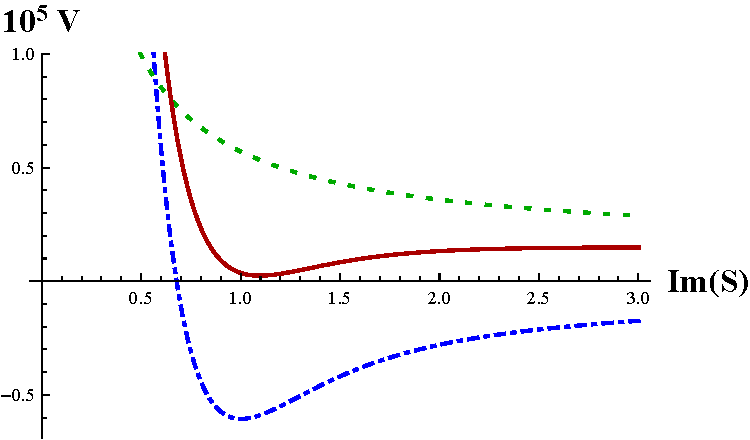
\includegraphics[scale=0.5]{d6bar_Si-direction_2D_NC_2.pdf}\hspace{10pt} 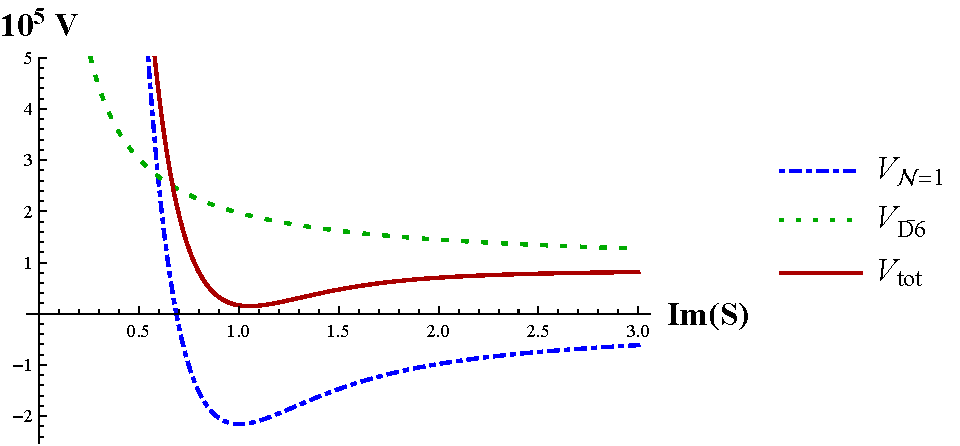
\includegraphics[scale=0.5]{d6bar_Si-direction_2D_2.pdf}\vspace{15pt}\\
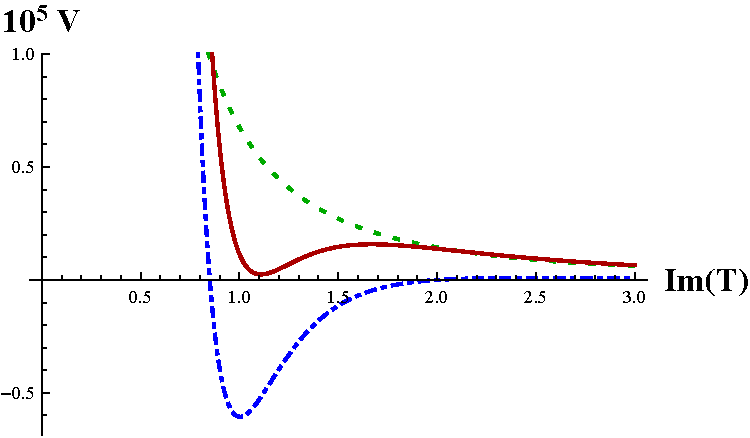
\includegraphics[scale=0.5]{d6bar_Ti-direction_2D_NC_2.pdf}\hspace{10pt} 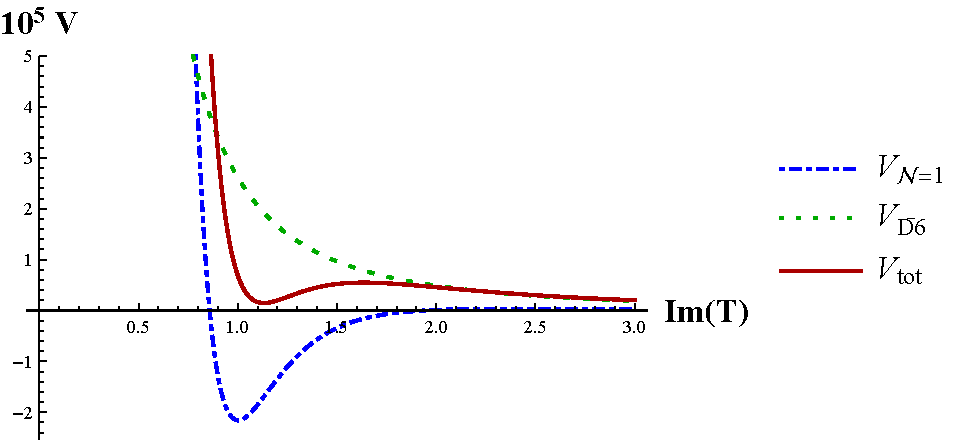
\includegraphics[scale=0.5]{d6bar_Ti-direction_2D_2.pdf}\vspace{15pt}\\
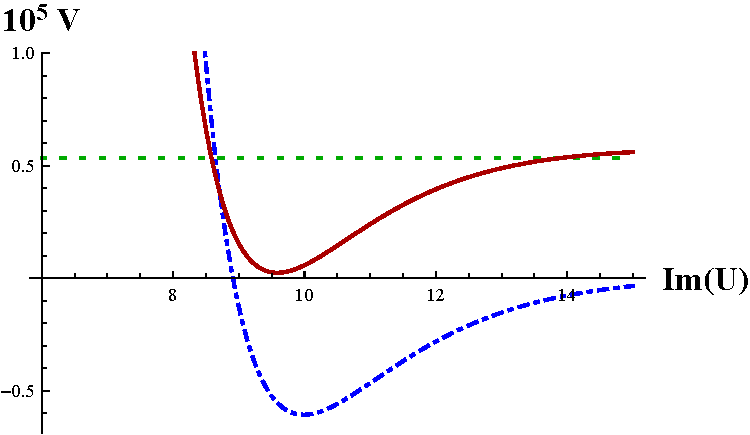
\includegraphics[scale=0.5]{d6bar_Ui-direction_2D_NC_2.pdf}\hspace{10pt} 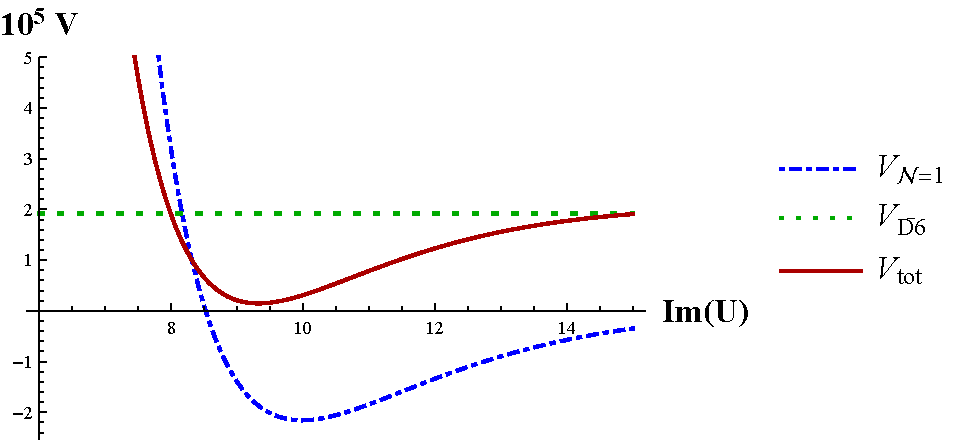
\includegraphics[scale=0.5]{d6bar_Ui-direction_2D_2.pdf}
\caption{Two dimensional plots showing the scalar potential in the AdS minimum (blue, dash-dotted), the contribution from the anti-D6-brane (green, dotted) and the resulting, total dS scalar potential (red, solid) for each direction in moduli space. The left side is for Set 1 and the right for Set 2.}
\label{fig:IIAupliftplot}
\end{figure}

\begin{figure}[H]
\hspace{100pt}
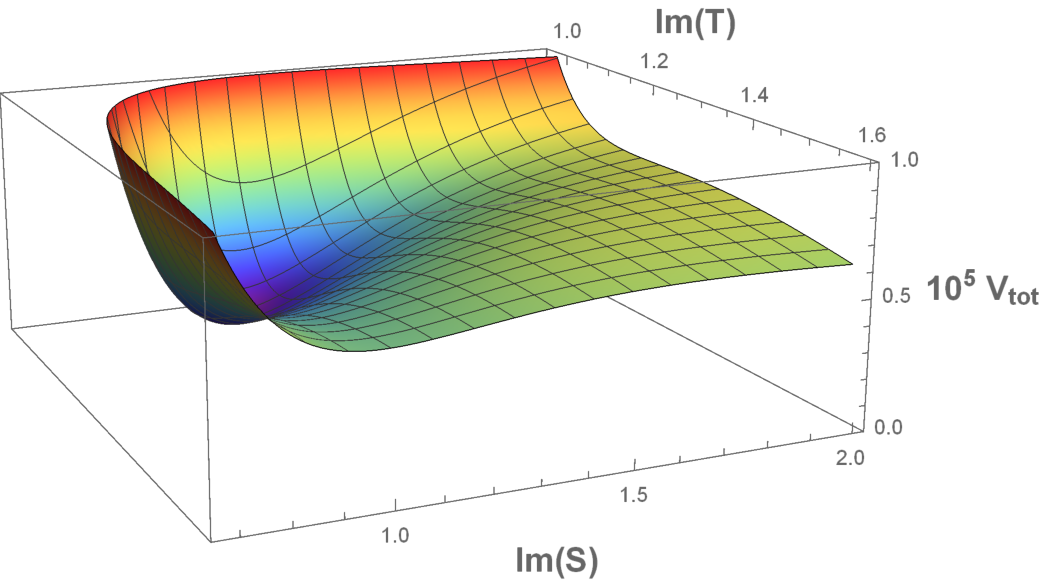
\includegraphics[scale=0.53]{d6bar_Si_and_Ti-directions_3D.pdf}\vspace{15pt}\\
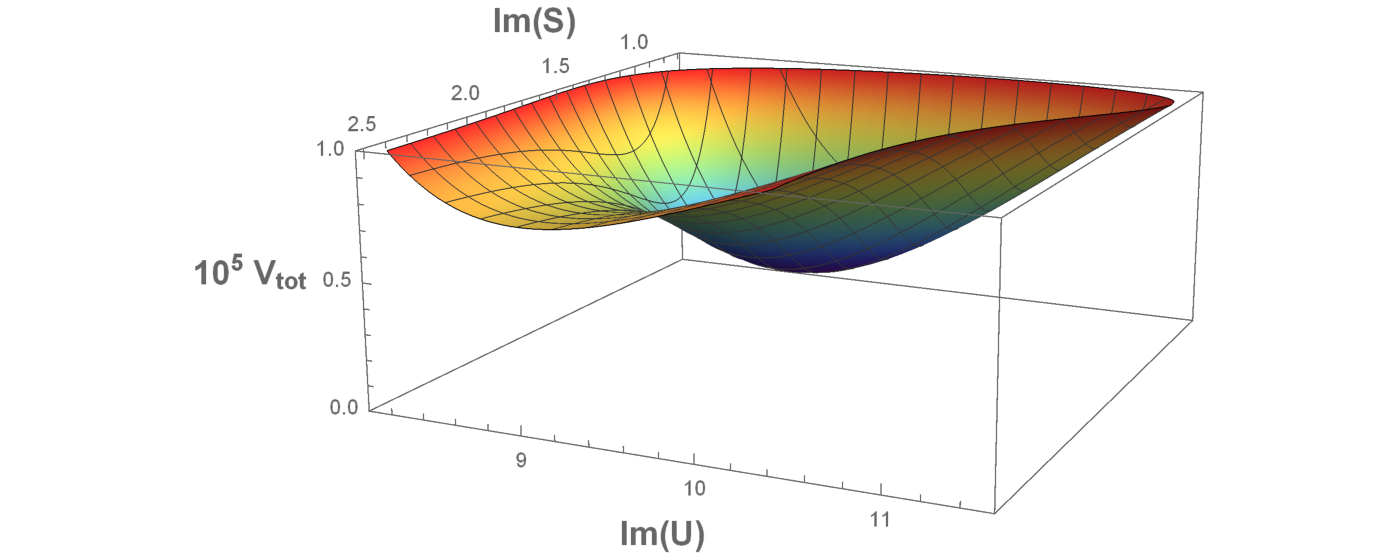
\includegraphics[scale=0.53]{d6bar_Si_and_Ui-directions_3D.pdf}\vspace{15pt}\\
\hbox{\hspace{50pt}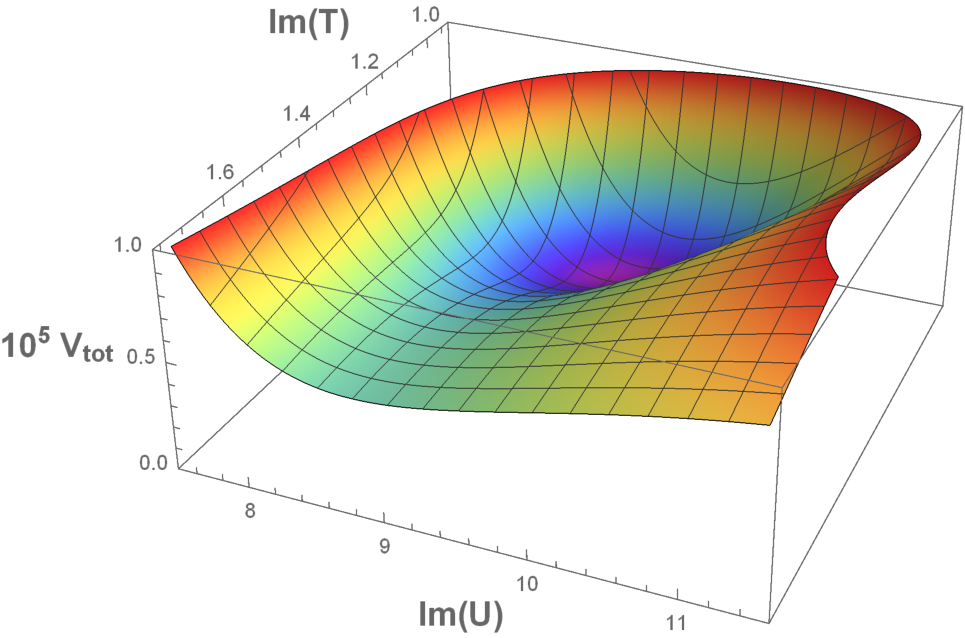
\includegraphics[scale=0.53]{d6bar_Ui_and_Ti-directions_3D.pdf}}
\caption{Three dimensional plots for Set 2, showing the (meta-) stability of the scalar potential. Top: Im$(S)$ and Im$(T)$, Middle: Im$(S)$ and Im$(U)$, Bottom: Im$(U)$ and Im$(T)$. }
\label{fig:IIAupliftplot3d}
\end{figure}

Two final remarks are in order. First, the parameters are not particularly fine-tuned, meaning that it was easy to find the two sets presented here. In fact, it is not hard to find even more examples. The only requirement is to keep the consistency conditions in mind. Second, this can be extended to a more general 7-moduli model. For this the moduli $T$ and $U$ split into three independent fields each. When having 7 independent directions the Kähler- and superpotential change to represent that fact in the following way:
\bea 
K&=  - \log\left(-\rmi (S-\bar{S})\right) - \sum_{i=1}^3  \log\left(-\rmi (T_i-\bar{T}_i)\right) - \sum_{i=1}^3 \log\left(-\rmi (U_i-\bar{U}_i)\right)\,,\\
W& = f_6 + A_{S}\, e^{\rmi a_S S} +  \sum_{i=1}^3 A_{T,i}\, e^{\rmi a_{T,i} T_i}+ \sum_{i=1}^3 A_{U,i}\, e^{\rmi a_{U,i} U_i}\,.
\eea
Furthermore, the contribution of the uplifting anti-D6-branes changes to represent the fact that there are now more cycles that can be wrapped:
\bea
V_{\overline{D6}} =\; &\frac{\mu_1^{\,4}}{Im(T_1)  Im(T_2)  Im(T_3)} +\frac{\mu_2^{\,4}}{Im(S)  Im(T_2)  Im(T_3)} \\+&\frac{\mu_3^{\,4}}{Im(S)  Im(T_1)  Im(T_3)} +\frac{\mu_4^{\,4}}{Im(S)  Im(T_1)  Im(T_2)}\,.
\eea
The procedure is otherwise analogous to what was done before. It is necessary to solve the 7 equations $D_IW=$ in terms of the parameters $A_S$, $A_{T,i}$ adn $A_{U,i}$. Then, using the remaining free coefficients, $S_0$, $T_{i,0}$, $U_{i,0}$, $f_6$, $a_S$, $a_{T,i}$ and $a_{U,i}$, one builds a stable anti-de Sitter minimum which gets lifted by the choice of the parameters $\mu_i$ ($i=1,2,3,4$) that correspond to the anti-D6-branes. Explicit examples are given in \cite{Cribiori:2019bfx} but are left out here since they do not provide any new insights.

\section{Mass Production of de Sitter Vacua in Type IIA and IIB}
\label{sec:massprod}
The method of the previous section is an easy way to obtain de Sitter vacua in type IIA supergravity models. However, there is no guarantee that one will arrive at a stable model following this procedure. In \cite{Kallosh:2019zgd} it was noted that it is possible to predict that the masses will stay positive during the procedure if one performs a detour by first going to Minkowski space. This allows to generate many meta-stable de Sitter vacua via an easy process. In this section we review the work done in \cite{Cribiori:2019drf}, where this procedure was supplied with explicit examples and generalized for use not only in IIA but also IIB settings.

\subsection{The mass Production Procedure}
The mass production procedure of meta-stable de Sitter vacua follows an easy 3-step process in $4d$, $\mathcal{N}=1$ supergravity:
\begin{enumerate}
\item Find a Minkowski progenitor model.
\item Downshift the model to anti-de Sitter via a perturbation to the superpotential.
\item Introduce anti-branes in order to perform an uplift to de Sitter.
\end{enumerate}
Following this path guarantees that the resulting de Sitter point is meta-stable under certain conditions.
Before going into the details of the construction some remarks are in order. \\
Finding a Minkowski minimum requires us to solve not only the equations $D_I W =0$, as we did before, but also $W=0$. This then leads to $\partial_I V=0$ and $V=0$ at the minimum. Not every possible superpotential allows for such solutions. Importantly, the model we investigated in the previous section, with $W = f_6 + \sum_I A_I \rme^{\rmi a_I \Phi_I}$ ($I = \{S,T,U\}$), cannot be  solved for Minkowski space. The models of \cite{Kallosh:2004yh,BlancoPillado:2005fn,Kallosh:2011qk}, however, are a generalization of our previous superpotential that do allow Minkowski vacua. These are called racetrack models and are schematically of the following form:
\be 
W = W_0 + \sum_I \left( A_I \rme^{\rmi a_I  \Phi^I} - B_I \rme^{\rmi b_I  \Phi^I}\right)\,.
\label{eq:racetrack}
\ee
Here we generalized the $f_6$ term of our type IIA models for use in general setups and the $\Phi^I$ represent all appearing moduli. It has been shown that models with such a superpotential can in fact produce Minkowski minima, as was shown in \cite{Kallosh:2019zgd,Kallosh:2004yh}. Thus, \eqref{eq:racetrack} will be the basis of our investigations in this section. We will go into detail about the Kallosh-Linde racetrack in section \ref{sec:KLmodel}.\\
The second step in our process, the AdS downshift, can be achieved via adding a small perturbation to the superpotential of the form $W_0 \to W_0 + \Delta W$. This will result in pushing a Minkowski vacuum with vanishing scalar potential at the minimum to an AdS vacuum with negative vacuum energy. For small downshifts this is expected to not change the position of the minimum too much and will not make the vacuum unstable.\\
Finally, the uplift follows as before and will lift the vacuum to de Sitter with positive vacuum energy. Note that we could have lifted starting from Minkowski space, however, this comes with an issue. Usually, one wants to match the cosmological constant in semi-realistic constructions. Since the cosmological constant is of order $10^{-120}$ an uplift from Minkowski to de Sitter would require an extreme amount of fine tuning. This can be alleviated by first going to anti-de Sitter. Then the uplift does not require as much fine tuning regarding the warping and/or amount of anti-D-branes.

\subsection{The Kallosh-Linde Racetrack Potential}
\label{sec:KLmodel}
The simplest Kähler- and superpotential we can write down in order to explain the procedure can be written as follows:
\bea 
K &=-3\log \left(-\rmi (\Phi - \bar{\Phi})\right) + X \bar{X}\,,\\
W &=W_0 + \Delta W +  A \rme^{\rmi a \Phi} - B \rme^{\rmi b \Phi} + \mu^2 X\,,
\label{eq:KLWandK}
\eea 
where $X$ is again a nilpotent chiral field that is used to include the uplifting contributions of anti-D-branes. The Minkowski solution is found by only considering $W_{KL} = W_0 +  A \rme^{\rmi a \Phi} - B \rme^{\rmi b \Phi}$.\\
To begin with, let us start by considering the Kallosh-Linde racetrack potential where we write the single field as $\Phi = \phi + \rmi \theta$. The solution to $W_{KL} = 0$ and $DW=0$ is given by
\bea
\Phi &= \phi = \frac{\rmi}{a-b} \log \frac{a\, A}{b\, B} \qquad \text{with}\\
W_0 &= -A\left(\frac{a\, A}{b\, B}\right)^{\frac{a}{b-a}} + B\left(\frac{a\, A}{b\, B}\right)^{\frac{b}{b-a}}\,,
\eea
where the axions have once again been set to zero. A solution to these equations exists for as long as $a>b$ and $a\,A > b\,B$. The mass of the field at the minimum evaluates to:
\be 
m_\Phi^2 = \frac{2\phi_0}{9} \left( W'' \right)^2 = \frac{2}{9}\, a\,A\,b\,B\,(a-b) \left( \frac{a\,A}{b\,B}\right)^{-\frac{a+b}{a-b}} \log \frac{a\, A}{b\,B}\,.
\ee
In order to go to AdS we now introduce a shift via $W_0 \to W_0 + \Delta W$. This changes the value of the scalar potential $V$ to:
\be 
V_{AdS} = - \frac{3(\Delta W)^2}{8 \phi_0^3} = -\frac{3}{8} \left(\frac{a-b}{\log \frac{a\, A}{b\,B}}\right)^3 (\Delta W)^2\,.
\ee
At leading order, this modification shifts the position of the vacuum in Moduli space only by 
\be 
\Delta \Phi = - \frac{K_\Phi \Delta W}{\partial_\Phi^2 W}\,.
\ee
Importantly, the changes, both in mass and position, depend on the tunable and small parameter $\Delta W$.\\
Now we can attempt to lift minimum, with a negative value for the cosmological constant, to a de Sitter point with nearly vanishing cosmological constant. This requires an uplift parameter of approximately
\be 
\mu^4 \approx 3 (\Delta W)^2\,.
\ee
Then, the gravitino mass in dS is given as
\be 
m_{3/2}^2 = \rme^K (\Delta W)^2 = \frac{(\Delta W)^2}{8 \phi_0^3} =  \frac{\mu^4}{24\phi_0^3}\,.
\ee
This model readily generalizes to more moduli and more exponents for each modulus. In the following we will use the model as given here but for $2$, $3$ or $7$ moduli.

\subsection{The Mass Matrix during the Mass Production Process}
\label{sec:massmass}
The most important claim of this section is that, given a Minkowski progenitor, we have a deterministic way to arrive at a meta-stable de Sitter vacuum. An important part of that claim is that masses in a supersymmetric Minkowski minimum are non-negative. This is discussed in detail in \cite{Kallosh:2019zgd}, based on earlier work from \cite{BlancoPillado:2005fn}. Here the arguments for this will briefly be summarized.\\
For this discussion it is useful to define a covariant, holomorphic superpotential, also called the complex gravitino mass as:
\be 
\rme^{K/2} W =: m(z^a,\bar{z}^{\bar{a}})\,,
\ee
which depends on on an arbitrary number of chiral matter superfields $z^a$. In terms of this quantity the real gravitino mass is $M_{3/2} = |m\bar{m}|$. The complex masses of the chiral fermions are then given to be
\be 
D_a D_b m =: m_{ab}\,,\qquad \bar{D}_{\bar{a}}\bar{D}_{\bar{b}}\bar{m} =: \bar{m}_{\bar{a}\bar{b}}\,.
\ee
Alternatively, this can be written as \cite{Freedman:2012zz}:
\be 
m_{ab} = \rme^{K/2} \left(\partial_a + K_a\right) D_b W - \rme^{K/2} \Gamma^{c}\,_{ab} D_c W\,.
\ee
\paragraph{For a supersymmetric Minkowski minimum,} $W = 0$ and $D_aW=0$, the expression for the fermion masses simplifies to
\be 
m_{ab}^{\text{Mink}} = \rme^{K/2} \partial_a \partial_b W\,.
\ee
Rewriting the scalar potential $V=\rme^K \left(|DW|^2 - 3 |W|\right)$ with this notation we find
\be 
V = m_a K^{a\bar{b}}\bar{m}_{\bar{b}} - 3 |m|^2 =: |m_a|^2 - 3 |m|^2\,,
\ee
where the Kähler metric is defined as $K_{a\bar{b}} = \partial_a \partial_{\bar{b}}K$. This scalar potential has an extremum for 
\be 
\partial_a V = -2 m_a \bar{m} + m_{ab} K^{b\bar{b}} \bar{m}_{\bar{b}}=0\,,
\ee
and it is supersymmetric if $m_a = \bar{m}_{\bar{b}}=0$. Note that non-supersymmetric extrema are possible as well for $2 m_a \bar{m} = m_{ab} K^{b\bar{b}} \bar{m}_{\bar{b}}$ with $m_a \neq 0$ and $\bar{m}_{\bar{b}} \neq 0$.\\
Writing the scalar mass-matrix as
\be 
\mathcal{M}^2 = \begin{pmatrix} V_{a\bar{b}} & V_{ab}\\V_{\bar{a}\bar{b}} & V_{\bar{a}b}\end{pmatrix}\,,
\ee
we can go on about our study of the behaviour of the masses under our mass production procedure. In a supersymmetric Minkowski vacuum the mass matrix becomes block diagonal
\be 
\left(\mathcal{M}^2\right)^{\text{Mink}} = \begin{pmatrix} V_{a\bar{b}}^{\text{Mink}} &0\\0 & V_{\bar{a}b}^{\text{Mink}}\end{pmatrix}\,,
\ee
with $V_{a\bar{b}}^{\text{Mink}} = m_{ac} K^{c\bar{c}}\bar{m}_{\bar{c}\bar{b}}$. Since the diagonal blocks are positive definite we conclude that all eigenvalues, corresponding to the masses of the scalars in our model, are non-negative. This can be further underlined by considering an arbitrary vector $\phi$:
\be 
\phi_a V_{a\bar{b}}^{\text{Mink}} \bar{\phi}_{\bar{b}} = \phi_a m_{ac} K^{c\bar{c}}\bar{m}_{\bar{c}\bar{b}} \bar{\phi}_{\bar{b}} = \Phi_c K^{c\bar{c}} \bar{\Phi}_{\bar{c}}\,,
\label{eq:MinkPosDef}
\ee
with $\Phi_c = \phi_a m_{ac}$. Since the Kähler metric $K^{c\bar{c}}$ is positive definite the same holds for the above combination. For the special choice of a racetrack superpotential \eqref{eq:KLWandK} the masses will in fact be strictly larger than zero and this property, as per the following discussion, will transfer to the resulting de Sitter minimum. 
\paragraph{Performing the downshift to Anti-de Sitter space} is done via the inclusion of a small shift in $W_0$: $W_0 \to W_0 +\Delta W$. Including such a term in the superpotential will yield an AdS minimum ($V<0$). This means that $D_aW=0$ will still be satisfied but not $W=0$. Likewise, the complex gravitino mass will no longer be zero:
\be 
m = \rme^K W \neq 0\,,
\ee 
while we still have 
\be 
m_a = 0\,.
\ee
The fermion mass matrix will no longer be block diagonal but due to the setup we can still quantify the change for a small shift $\Delta W$. Under this change the Kähler potential will be unaffected. When necessary we will distinguish the quantities by superscripts Mink and AdS. To investigate the AdS masses we consider the change of the position of the minimum: $z_a^{\text{Mink}} \to z_a^{\text{AdS}}$. We still have unbroken supersymmetry which leads, at leading order, to
\be 
\delta z^a = - (m_{ab})^{-1} K_b \Delta m + \cdots\,.
\ee
The change in the complex gravitino mass is $\Delta m = \rme^{K/2} \Delta W$. For the position of the minimum the change is small if $\Delta m$ is smaller than the smallest eigenvalue of the fermion mass matrix $m_\chi$. The fermion mass matrix in AdS at the point $z + \delta z$ can be written as
\be 
V_{a\bar{b}}^{\text{AdS}}=m_{ac}K^{c\bar{c}}-2K_{a\bar{b}} m \bar{m}\,.
\ee
The first part is still positive definite, as in the Minkowski case. We immediately see that the AdS minimum will be (meta-)stable if the gravitino mass is smaller than the lightest eigenvalue of the Minkowski fermion mass matrix:
\be 
m_{\chi} \gg m_{3/2}\,.
\ee
If this condition is satisfied we are certain to find a stable, supersymmetric anti-de Sitter vacuum by performing a shift in the superpotential from a previously known Minkowski progenitor.
\paragraph{Under the uplift to de Sitter} we likewise need to check what happens to the position of the minimum and the masses of the model. The lift to dS is perfromed by including a nilpotent, chiral field $X$ into the Kähler- and superpotential as in equations \eqref{eq:KLWandK}. Because of $X$ we now have new contributions to the scalar potential and mass matrix. We will include them by using the index $I = \{a,X\}$. The de Sitter scalar potential is
\be 
V^{\text{dS}} = \rme^K \left(|D_IW|^2-3|W|^2\right) = |m_I|^2 - 3 |m|^2 >0\,.
\ee
All new contributions have been included by our change of the index. For a successful uplift the supersymmetry breaking terms in $|m_I|^2$ need to be larger than the gravitino mass. The holomorphic/anti-holomorphic part of the mass matrix now evaluates to \cite{Denef:2004ze,Kallosh:2014oja}:
\be 
V_{a\bar{b}}^{\text{dS}}=m_{aI} K^{I\bar{J}} \bar{m}_{\bar{J}\bar{b}} - 2 K_{a\bar{b}}m_I \bar{m}^I - R_{a\bar{b}I\bar{I}} \bar{m}^I m^{\bar{I}} - m_a \bar{m}_{\bar{b}}\,.
\label{eq:dSmassmatrix}
\ee
Here, we have not considered the $X$ direction in moduli space since they are fundamentally fermionic in nature. Furthermore, $R_{a\bar{b}I\bar{I}}$ is the moduli space curvature tensor. The holomorphic/holomorphic part of the mass matrix in de Sitter reads:
\be 
V_{ab}^{\text{dS}} = -m_{ab}\bar{m} + m_{abI} \bar{m}^I\,.
\ee
Once again, we will consider the mass change due to the introduction of the new contribution in terms of the shift of the minimum. For this we consider the AdS minimum at $z^{a,\,\text{AdS}} = z^{a,\,\text{AdS}}_r + \rmi z^{a,\,\text{AdS}}_i$ and then the change will be due to the uplfiting contribution in the scalar potential:
\be 
V^{\text{up}} = \mu^4 \rme^K K_{X\bar{X}}\,.
\ee
The de Sitter minimum is located at 
\be 
\partial_{z^a_{\alpha}} \left[V^{\text{AdS}} + V^{\text{up}}\right] =0\,,
\ee
where $\alpha = \{i,\,r\}$. Using our knowledge about the AdS minimum and the uplift potential we find for the two terms individually:
\be 
\partial_{z^a_{\alpha}} V^{\text{AdS}}=\left(\partial_{z^a_\alpha } \partial_{z^b_\beta} V^{\text{AdS}} \right) \delta z^b_\beta\,, \qquad \partial_{z^a_{\alpha}} V^{\text{up}} = \mu^4 \partial_{z^a_\alpha} \left(\rme^K K_{X\bar{X}}\right)\,.
\ee
With this we can express the shift of the minimum, when going from AdS to dS as:
\be 
\delta z^b_\beta = -\left( \partial_{z_\alpha^a}\partial_{z^b_\beta} V^{\text{AdS}}\right)^{-1} \mu^4 \partial_{z^a_\alpha} \left(\rme^K K_{X\bar{X}}\right)\,.
\ee
Since the uplift is of the same order as the downshift we know that the masses $\partial_{z\alpha^a}\partial_{z^b_\beta} V^{\text{AdS}}$ are larger than the scale of the uplift and thus the shift of the position of the minimum will likewise be small. Using this result we furthermore find that the amount of supersymmetry breaking in direction of the unconstrained moduli is small compared to the nilpotent one \cite{Linde:2011ja}:
\be 
|m_a|^2 \ll |m_X|^2\,.
\ee
For stability of the de Sitter minimum we require the amount of supersymmetry breaking to be small compared to the chiral masses. We thus have, together with our earlier requirement that the gravitino mass is parametrically small, for a positive value of the potential at the minimum the following conditions:
\be 
m_\chi \gg |m_I|^2\qquad m_\chi^2 \gg m^2_{3/2} \qquad |m_I|^2 > 3 m_{3/2}^2\,,
\label{eq:dSstabcond}
\ee
where $m_\chi$ is once again the smallest eigenvalue of the mass matrix. As observed before, supersymmetry breaking in the chiral directions is very small and thus SUSY breaking in the nilpotent direction is of the order of the gravitino mass for almost vanishing cosmological constant.\\
Finally, we have to consider the mass matrix \eqref{eq:dSmassmatrix}. The first term is positive definite and will be strictly positive if the progenitor Minkowski space has no flat directions. Because of the conditions in \eqref{eq:dSstabcond}, all other terms in \eqref{eq:dSmassmatrix} are parametrically small and thus we conclude that the de Sitter mass matrix will be positive definite, or in the case of a Minkowski progenitor without flat directions, it will have strictly  positive eigenvalues. With this we have shown how to obtain a (meta-) stable dS vacuum from our mass production procedure.

\subsection{Model Choices in type IIA and IIB}
The discussion up until this point has been about fairly general Kähler- and superpotentials. By considering specific choices the we can find stronger bounds on the masses in our de Sitter model. In the following sections we will show explicit examples in detail that are based on the choices of $K$ and $W$ we discuss in this section. 
\paragraph{For type IIA} we consider models based on the superpotentials that were already studied in \cite{Kallosh:2019zgd}:
\bea 
K &= - \sum_{I=1}^n N_I \log \left( -\rmi (\Phi^I - \bar{\Phi}^I )\right)\,,\\
W &= W_0 + \sum_{I=1}^n \left( A_I \rme^{\rmi a_I \Phi^I} - B_I \rme^{\rmi b_I \Phi^I} \right)\,.
\label{eq:IIAKW}
\eea 
Here, $\Phi^i$ runs over all the moduli we are considering and and $W_0$, $a_I$, $b_I$, $A_I$, $B_I$ and $N_I$ are real parameters. For this class of models we find that the mass matrix is diagonal when splitting the moduli as $\Phi^I = \phi^I + \rmi \theta^I$ with the $\phi^I$ and $\theta^I$ real:
\be 
\begin{pmatrix}
V_{\phi^I\phi^J} & V_{\phi^I \theta^J}\\
V_{\theta^I\phi^J} & V_{\theta^I \theta^J}
\end{pmatrix}\Bigg|_{\text{Mink}}
=
\begin{pmatrix}
m^2_{\phi^I\phi^I} & 0\\
0 & m^2_{\theta^I \theta^I}
\end{pmatrix}\,.
\ee
Furthermore, there is a mass degeneracy between the scalars and pseudo-scalars:
\be 
m^2_{\phi^I\phi^I} = m^2_{\theta^I \theta^I}\,.
\ee
When perturbing the model in order to go to an anti-de Sitter Minimum by a small $\Delta W$, the mass matrix will remain block-diagonal:
\be 
\begin{pmatrix}
V_{\phi^I\phi^J} & V_{\phi^I \theta^J}\\
V_{\theta^I\phi^J} & V_{\theta^I \theta^J}
\end{pmatrix}\Bigg|_{\text{AdS}}
=
\begin{pmatrix}
V^{\text{Mink}}_{\phi^I\phi^J} + \Delta_{\phi^I \phi^J}& 0\\
0 & V^{\text{Mink}}_{\theta^I \theta^J}+\Delta_{\theta^I \theta^J}
\end{pmatrix}\,.
\ee
Note that the terms $\Delta_{\phi^I \phi^J}$ and $\Delta_{\theta^I \theta^J}$ can appear in the off-diagonals but, as per our previous analysis, they are parametrically small compared to the diagonal terms. Now, if we introduce the uplift, as discussed above, we will change the mass matrix one more time, however, by another parametrically small amount:

\be 
\begin{pmatrix}
V_{\phi^I\phi^J} & V_{\phi^I \theta^J}\\
V_{\theta^I\phi^J} & V_{\theta^I \theta^J}
\end{pmatrix}\Bigg|_{\text{dS}}
=
\begin{pmatrix}
V^{\text{Mink}}_{\phi^I\phi^J} + \Delta_{\phi^I \phi^J}+ \tilde{\Delta}_{\phi^I \phi^J}& 0\\
0 & V^{\text{Mink}}_{\theta^I \theta^J}+\Delta_{\theta^I \theta^J}+\tilde{\Delta}_{\theta^I \theta^J}
\end{pmatrix}\,.
\ee
Since all the contributions to the mass matrix during the mass production procedure are small we conclude that we should find $V^{\text{dS}}_{IJ} \approx V^{\text{Mink}}_{IJ}$, where $I$ and $J$ symbolically stand for the fields $\phi^I$ and $\theta^I$. Furthermore, due to the the mass degeneracy in Minkowski we also expect that in AdS and dS at least an approximate mass degeneracy is present.
\paragraph{In type IIB} the superpotential will be the same as in the type IIA case \eqref{eq:IIAKW}. The Kähler potential, on the other hand, will differ and in general be of the form:
\be 
K = K\left(-\rmi ( \Phi^I - \bar{\Phi}^I )\right)\,.
\ee 
One immediate consequence of this is that already the Minkowski mass matrix is now only block-diagonal, instead of diagonal:
\be 
V_{IJ}|_{\text{Mink}}=
\begin{pmatrix}
V_{\phi^I\phi^J} & 0\\
0 & V_{\theta^I \theta^J}
\end{pmatrix}\,.
\ee
Still, due to \eqref{eq:MinkPosDef}, this matrix is positive definite and there will be still a mass degeneracy between the scalars and pseudo-scalars. Nevertheless, the same arguments as in type IIA hold and the changes in the masses in the process of going from Minkowski space to de Sitter will be small.

\subsection{Explicit Examples in type IIA}
\label{sec:massIIAexampel}
In this section two explicit examples in type IIA will be presented. We will discuss the seven moduli example and its simplification, the STU model. More details can be found in \cite{Cribiori:2019drf}, from which the numerical data and plots were taken as well.
\paragraph{The Seven-Moduli model in IIA} exhibits an $SL[(2,\mathbb{R})]^7$ symmetry and is closely related to M-theory models and $d=4$, $\mathcal{N}=8$ supergravity. These models were constructed from compactifying from $10$ to $4$ on $T^6/(\mathbb{Z}_2 \times \mathbb{Z}_2)$ in \cite{Derendinger:2004jn,Villadoro:2005cu} and are in particular interesting for future B-mode experiments as discussed in \cite{Ferrara:2016fwe,Kallosh:2017ced}. The model includes the seven moduli:
\be 
\Phi^I = \{S,T_1,T_2,T_3,U_1,U_2,U_3\}\,,
\ee
where $S$ is the axio-dilaton, the $T_i$ ($i=1,2,3$) are the complex structure moduli and the $U_i$ are the Kähler moduli. The $\Phi^I$ are in a sense the coordinates of the $[SL(2,\mathbb{R})/U(1)]^7$ coset. The Kähler- and superpotential for our example are:
\bea 
\label{eq:massIIA7modpot}
K &= - \sum_I \log \left(-\rmi (\Phi^I -\bar{\Phi}^I)\right)\,,\\
W &= f_6 + \sum_I \left( A_I \rme^{\rmi a_I \Phi^I} - B_I \rme^{\rmi b_I \Phi^I} \right)\,,
\eea 
where we will utilize the Kallosh-Linde racetrack superpotential. Once again, we do not consider P-fluxes other than $F_6$. The shift to anti-de Sitter is performed by letting $f_6 \to f_6 + \Delta f_6$. The contribution of the uplift to the scalar potential due to the anti-D6-brane uplift is
\bea
V_{\overline{D6}}^{\text{up}} =\; & \frac{\mu_0^4}{\rmim(T_1)\rmim(T_2)\rmim(T_3)} + \frac{\mu_1^4}{\rmim(S)\rmim(T_2)\rmim(T_3)} \\+ & \frac{\mu_2^4}{\rmim(S)\rmim(T_1)\rmim(T_3)} + \frac{\mu_3^4}{\rmim(S)\rmim(T_1)\rmim(T_2)}\,,
\eea
which can, again, be obtained using a nilpotent field $X$ \cite{Kallosh:2018nrk,Cribiori:2019bfx}. As is evident, we have now several cycles around which the anti-branes can be wrapped around and the parameters $\mu_i^4$ can, but do not need to be, tuned individually.\\
In order to find solutions to the equations $D_I W =0$ and $W=0$, which will give a Minkowski minimum, we use the parameters $B_I$ and $f_6$. Thus, we can freely choose the point in moduli space and the parameters $A_I$, $a_I$ and $b_I$. The choices are given in table \ref{tab:7modchoice}. Once again, we set the axions to zero which will not produce any problems as discussed in section \ref{sec:uplfitbraneexamples}. The position of the Minkowski minimum will thus be at $S=\rmi \,S_0$, $T_i = \rmi \,T_{i,0}$ and $U_i = \rmi \,U_{i,0}$ where $i=1,2,3$.\\
In choosing the parameters we had to keep the same requirements in mind as in section \ref{sec:antibraneupSTU}.  Namely, $a_I \Phi^I$ needs to be small such that higher-order corrections can safely be neglected and we choose the $U_i$ large in order to obtain a large internal volume. Other than that, no particular care is required in choosing these parameters. Even with these conditions it is relatively easy to find positive masses, meaning that the parameters are not particularly fine-tuned. For the downshift parameter we choose 
\be 
\Delta f_6 = -10^{-5}\,.
\ee 
The sign of this parameter does matter and can change the behaviour but, for small downshifts, the qualitative effect will be independent of the sign. For the uplift we set all the parameters to be equal:
\be 
\mu_0 ^4 = \mu_1 ^4 = \mu_2 ^4 = \mu_3 ^4 = 5.49028 \cdot 10^{-15}\,.
\ee
\begin{table}[H]
\centering
\begin{tabular}{|c|c|c|c|c|c|c|}\hline
$A_S = 1$ & $A_{T_1} = 3.1$& $A_{T_2} = 3.2$& $A_{T_3} = 3.3$ & $A_{U_1} =11$& $A_{U_2} =12$& $A_{U_3} =13$\\\hline
$a_S = 2$ & $a_{T_1} = 2.1$& $a_{T_2} = 2.2$& $a_{T_3} = 2.3$ & $a_{U_1} =0.41$& $a_{U_2} =0.42$& $a_{U_3} =0.43$\\\hline
$b_S = 3$ & $b_{T_1} = 3.1$& $b_{T_2} = 3.2$& $b_{T_3} = 3.3$ & $b_{U_1} =1.1$& $b_{U_2} =1.2$& $b_{U_3} =1.3$\\\hline
$S_0 = 1$ & $T_{1,\,0} = 1.1$  & $T_{2,\,0} = 1.2$  & $T_{3,\,0} = 1.3$ & $U_{1,\,0} = 5.1$& $U_{2,\,0} = 5.2$& $U_{3,\,0} = 5.3$\\\hline
\end{tabular}
\caption{Choices for the position in moduli space and parameters in the 7-moduli example in type IIA.}
\label{tab:7modchoice}
\end{table}
The value chosen here, and in the following, have not been selected to match the observed cosmological constant but rather for illustrative purposes. With the choices in table \ref{tab:7modchoice} one obtains a Minkowski minimum with strictly positive values for the masses and thus, as by our prior discussion, the same should hold for the de Sitter masses. We give both, the Minkowski and de Sitter, masses in table \ref{tab:7modmass}. The change in masses is noticeable but small, as predicted. Furthermore, the mass degeneracy is also broken in Minkowski, to a minute degree. In addition to its eigenvalues, below the upper right corner block of the dS Mass matrix is shown. It is evident that the off-diagonal terms are much smaller than the diagonal entries, visualizing our discussion from section \ref{sec:massmass}.\\
Due to the sheer amount of plots necessary do properly represent the 7-moduli example we instead will use the related STU-model in order  to visualize the behaviour.

{\tiny
\begin{equation}
 \left(
\begin{array}{ccccccc}
1.89809 \cdot 10^{-5} & -6.19837 \cdot 10^{-10} &- 5.36624 \cdot 10^{-10}& -4.56280 \cdot 10^{-10} & -1.30375 \cdot 10^{-9}& -1.52470 \cdot 10^{-9} & -1.74268 \cdot 10^{-9}\\
\\
-6.19837 \cdot 10^{-10} & 1.30911 \cdot 10^{-4} & -7.38721 \cdot 10^{-10} & -6.46383 \cdot 10^{-10} & -1.24516 \cdot 10^{-9} & -1.44398 \cdot 10^{-9} & -1.64104 \cdot 10^{-9}\\
\\
-5.36624 \cdot 10^{-10} & -7.38721 \cdot 10^{-10} & 9.41667 \cdot 10^{-5} & -5.68241 \cdot 10^{-10} & -1.13520 \cdot 10^{-9} &-1.31758 \cdot 10^{-9} &-1.49834 \cdot 10^{-9}\\
\\
-4.56280 \cdot 10^{-10} & -6.46383 \cdot 10^{-10} & -5.68241 \cdot 10^{-10} &6.37888 \cdot 10^{-5}&-1.04022 \cdot 10^{-9}& -1.20871 \cdot 10^{-9}&-1.37571 \cdot 10^{-9}\\
\\
-1.30475 \cdot 10^{-9} & -1.24516 \cdot 10^{-9} & -1.13520 \cdot 10^{-9} & -1.04022 \cdot 10^{-9} & 9.96472 \cdot 10^{-4} &-5.36645 \cdot 10^{-10} & -5.74900 \cdot 10^{-10}\\
\\
-1.52470 \cdot 10^{-9}&-1.44398 \cdot 10^{-9}& -1.31758 \cdot 10^{-9}& -1.20871 \cdot 10^{-9 }&-5.36646 \cdot 10^{-10} & 1.37262 \cdot 10^{-3}& -6.10079 \cdot 10^{-10}\\
\\
-1.74268 \cdot 10^{-9}& -1.64104 \cdot 10^{-9}& -1.49834 \cdot 10^{-9} & -1.37571 \cdot 10^{-9}& -5.74900 \cdot 10^{-10} &-6.10079 \cdot 10^{-10}&1.80465 \cdot 10^{-3}
\end{array}
\right)\nonumber
\end{equation}
}

\begin{table}[htb]
\centering
\begin{tabular}{|c|c|c|c|}\hline
& Minkowski  & de Sitter \\\hline
$m_1^{\,2}$   & $\;1.80473 \cdot 10^{-3}\;$  & $\;1.80465 \cdot 10^{-3}\;$\\\hline
$m_2^{\,2}$   & $1.80473 \cdot 10^{-3}$  & $1.80465 \cdot 10^{-3}$\\\hline
$m_3^{\,2}$   & $1.37269 \cdot 10^{-3}$  & $1.37262 \cdot 10^{-3}$\\\hline
$m_4^{\,2}$   & $1.37269 \cdot 10^{-3}$  & $1.37262 \cdot 10^{-3}$\\\hline
$m_5^{\,2}$   & $9.96519 \cdot 10^{-4}$  & $9.96472 \cdot 10^{-4}$\\\hline
$m_6^{\,2}$   & $9.96519 \cdot 10^{-4}$  & $9.96471 \cdot 10^{-4}$\\\hline
$m_7^{\,2}$   & $1.30924 \cdot 10^{-4}$  & $1.30911 \cdot 10^{-4}$\\\hline
$m_8^{\,2}$   & $1.30924 \cdot 10^{-4}$  & $1.30911 \cdot 10^{-4}$\\\hline
$m_9^{\,2}$   & $9.41773 \cdot 10^{-5}$  & $9.41667 \cdot 10^{-5}$\\\hline
$m_{10}^{\,2}$& $9.41773 \cdot 10^{-5}$  & $9.41660 \cdot 10^{-5}$\\\hline
$m_{11}^{\,2}$& $6.37973 \cdot 10^{-5}$  & $6.37888 \cdot 10^{-5}$\\\hline
$m_{12}^{\,2}$& $6.37973 \cdot 10^{-5}$  & $6.37883 \cdot 10^{-5}$\\\hline
$m_{13}^{\,2}$& $1.89843 \cdot 10^{-5}$  & $1.89809 \cdot 10^{-5}$\\\hline
$m_{14}^{\,2}$& $1.89843 \cdot 10^{-5}$  & $1.89806 \cdot 10^{-5}$\\\hline
\end{tabular}
\caption{  The masses in Minkowski and de Sitter for the 7 moduli IIA example. The changes during the procedure are small but noticeable. A very small deviation from the mass degeneracy, originally present in Minkowski space, is visible. }
\label{tab:7modmass}
\end{table}

\FloatBarrier
\paragraph{The IIA STU model} is a simplification of the above case where one identifies the different complex structure and Kähler moduli:
\be 
T_i \to T\,, \qquad U_i \to U\,, \qquad \text{for }\,i=1,2,3\,.
\ee
The model is then very similar to the model of section \ref{sec:antibraneupSTU} but with the racetrack superpotential. The Kähler- and superpotential are:
\bea 
K &= -\log \left( -\rmi (S-\bar{S})\right) - 3 \log \left( -\rmi (T-\bar{T})\right)- 3 \log \left( -\rmi (U-\bar{U})\right)\,,\\
W &= f_6 \,+ \sum_{\Phi = S,T,U} \left( A_\Phi \rme^{\rmi a_\Phi \Phi} - B_\Phi \rme^{\rmi b_\Phi \Phi}\right)\,.
\eea
The uplift contribution to the scalar potential in this model likewise simplifies to
\be 
V_{\overline{D6}}^{\text{up}} =  \frac{\mu_0^4}{\rmim(T)^3} + \frac{\mu_1^4}{\rmim(S)\rmim(T)^2} \,.
\ee
Finding solutions to this proceeds as before by first setting the axions to zero and then solving in terms of $f_6$ and the $B_I$, while the other parameters remain free and are listed in table \ref{tab:stupara}.
\begin{table}[H]
\centering
\begin{tabular}{|c|c|c|}\hline
$A_S = 1$ & $A_T = 3$ & $A_U =11$\\\hline
$a_S = 2$ & $a_T = 2.1$ & $a_U = 1$\\\hline
$b_S = 3$ & $b_T = 3.1$ & $b_U = 1.2$\\\hline
$S_0 = 1$ & $T_0 = 1$ & $U_0 = 5$\\\hline
\end{tabular}
\caption{   Our choice of parameters for the 3 moduli IIA example.}
\label{tab:stupara}
\end{table}
The downshift, once again, is
\be 
\Delta f_6 = -10^{-5}\,,
\ee 
while the uplift is 
\be 
\mu_0^4 = \mu_1^4 = 1.93753 \cdot 10^{-14}\,.
\ee
The resulting masses are given in table \ref{tab:stumass}, where we see once more that the masses change only slightly and the mass degeneracy breaks in de Sitter space.
\begin{table}[htb]
\centering
\begin{tabular}{|c|c|c|c|}\hline
&  Minkowski  & de Sitter \\\hline
$m_1^{\,2}$ & $\; 9.91957 \cdot 10^{-5} \;$ & $\; 9.91570 \cdot 10^{-5} \;$ \\\hline
$m_2^{\,2}$ & $\; 9.91957 \cdot 10^{-5} \;$ & $\; 9.91551 \cdot 10^{-5} \;$ \\\hline
$m_3^{\,2}$ & $\; 3.66313 \cdot 10^{-5} \;$ & $\; 3.66189 \cdot 10^{-5} \;$ \\\hline
$m_4^{\,2}$ & $\; 3.66313 \cdot 10^{-5} \;$ & $\; 3.66183 \cdot 10^{-5} \;$ \\\hline
$m_5^{\,2}$ & $\; 9.15565 \cdot 10^{-7} \;$ & $\; 9.14587 \cdot 10^{-7} \;$ \\\hline
$m_6^{\,2}$ & $\; 9.15565 \cdot 10^{-7} \;$ & $\; 9.14550 \cdot 10^{-7} \;$ \\\hline
\end{tabular}
\caption{  Values for the masses in Minkowski and de Sitter for the STU-model. As in the 7-moduli case the change in  going from Minkowski do de Sitter is evident as well as the breaking of the mass degeneracy.}
\label{tab:stumass}
\end{table} For this model we illustrate the behavior via some exemplary plots. In figure \ref{fig:stushift} one can see that the position of the minimum shifts slightly under the procedure. In figure \ref{fig:stu3Dlarge} the form of the potential for the $\rmim(S)$ and $\rmim(T)$ directions is shown. The meta-stability of the minimum in these directions is evident. Similar plots can be obtained for the other directions. Finally, in figure \ref{fig:stu3Dclose} a close-up of the minimum, both in AdS and dS, for the same directions is depicted. The hole seen there is the part in AdS with negative values for the potential.
\begin{figure}[htb]
\center
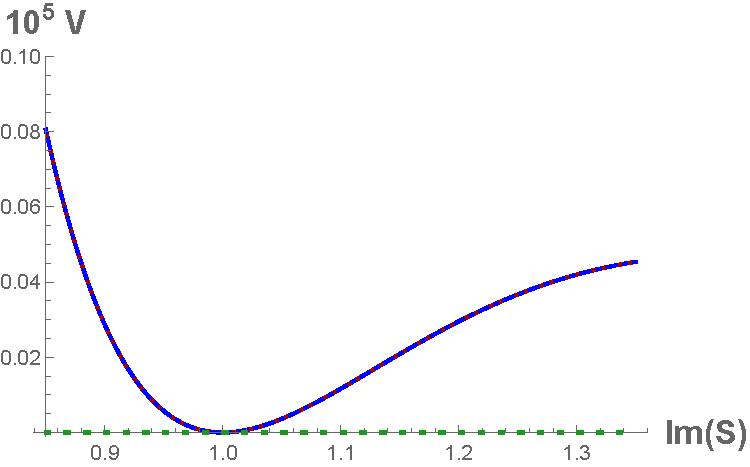
\includegraphics[scale=0.52]{3ModdsShift.pdf}\qquad
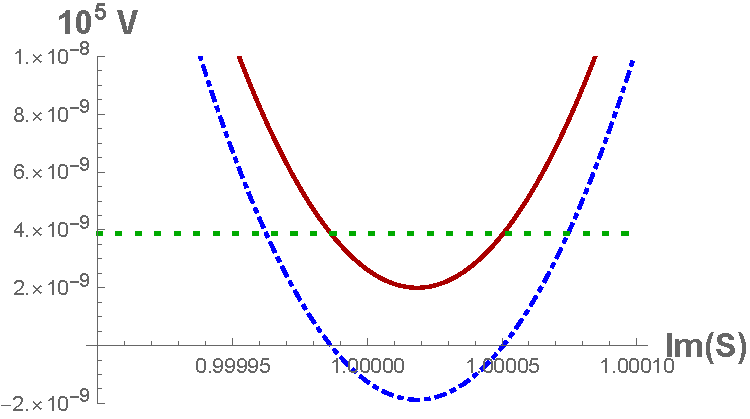
\includegraphics[scale=0.52]{3ModdsShift_close.pdf}
\caption{ The shift of the position of the minimum in the IIA STU-model when going from AdS to dS for the $\rmim(S)$ direction. On the left the AdS and dS scalar potential visually overlapp while the anti-brane contribution seems to be at zero. In the close-up on the right the differences become visible. The anti-D6-brane gives a flat contribution in this direction (dotted, green) and it is evident that the position of the minimum moves slightly when going from AdS (dash-dotted, blue) to dS (solid, red).}
\label{fig:stushift}
\end{figure}
\begin{figure}[htb]\hskip 2cm
%\begin{center}
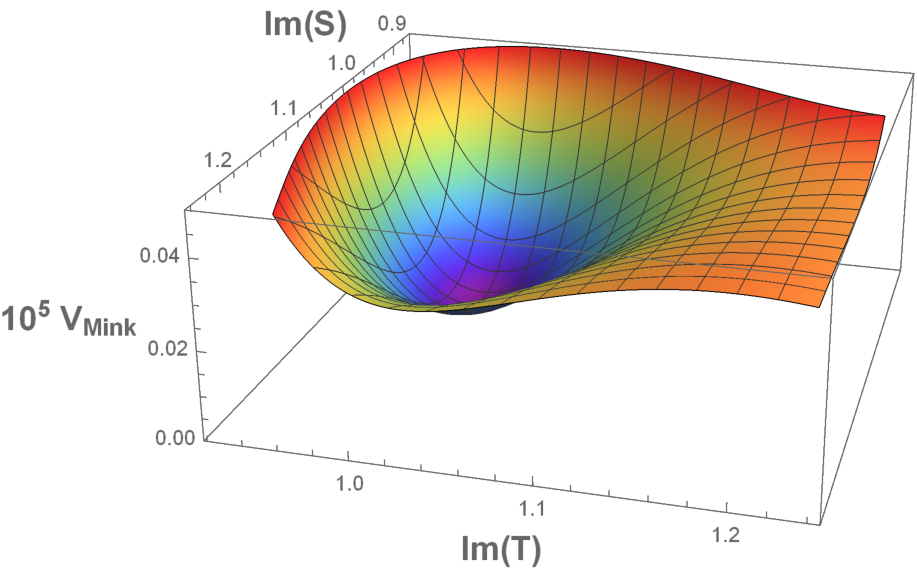
\includegraphics[scale=0.6]{3Mod3DLarge.pdf}
%\end{center}
\caption{ The $\rmim(S)$ and $\rmim(T)$ 3D slice of the scalar potential in the IIA STU-model. The potential is shows a meta-stable behaviour around the minimum. The form of this  potential, and the other possible slices, does not change significantly during the 3 steps of the procedure.}
\label{fig:stu3Dlarge}
\end{figure}
\begin{figure}[htb]
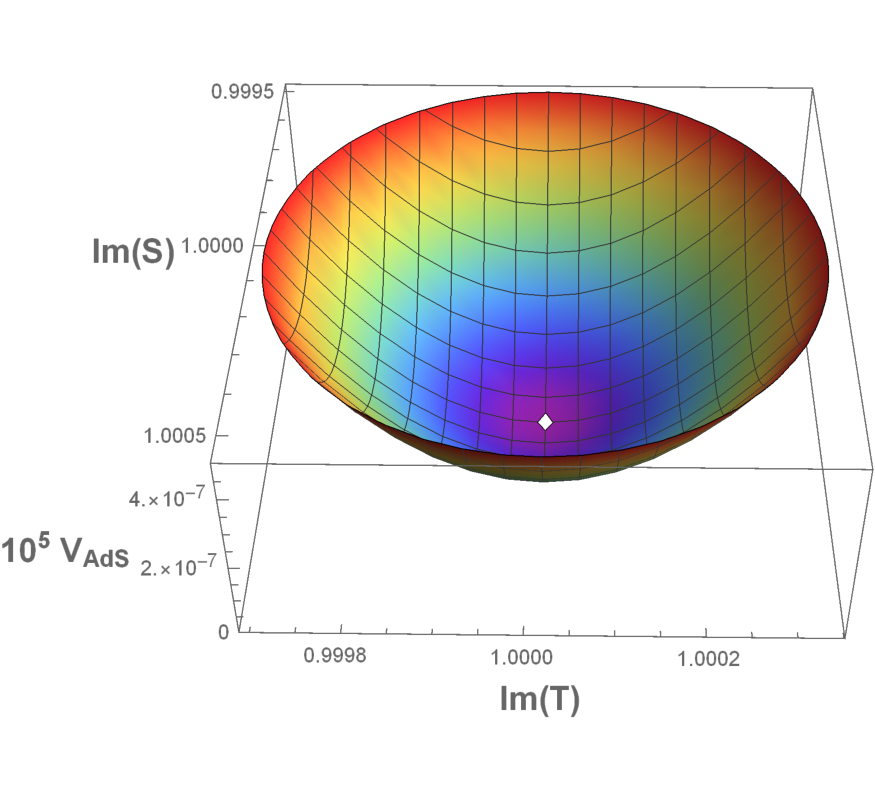
\includegraphics[scale=0.457]{3Mod3DAdS.pdf} 
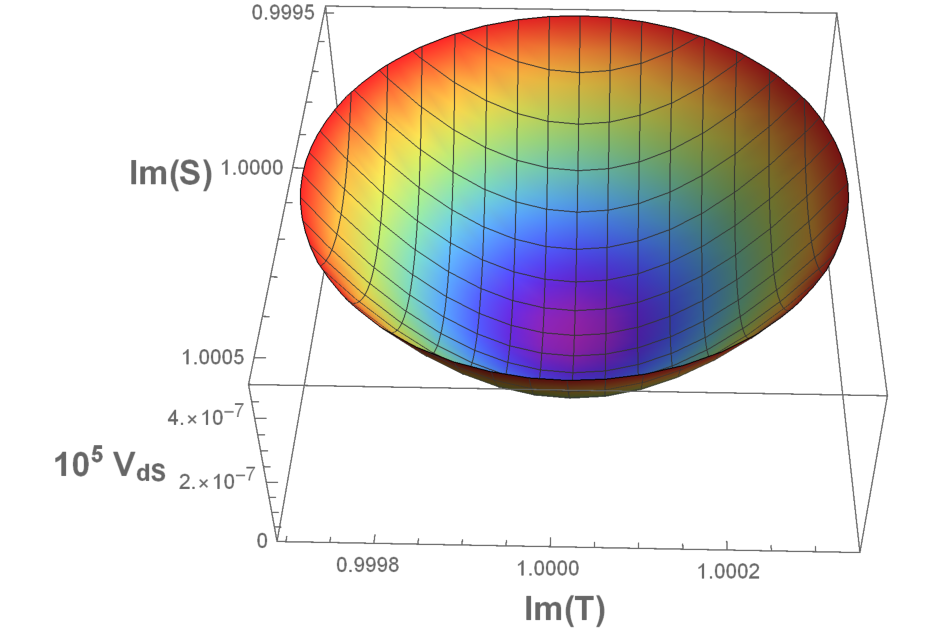
\includegraphics[scale=0.46]{3Mod3DdS.pdf}
\caption{  The minimum of the scalar potential in the $\rmim(S)$ and $\rmim(T)$ slice of the IIA STU-model. On the left the parts of the potential with negative values is visible as the hole. On the right the whole of the potential is now positive due to the uplift term. }
\label{fig:stu3Dclose}
\end{figure}


\FloatBarrier
\subsection{Explicit Examples in type IIB}
In type IIB we focus on models already investigated in \cite{Cicoli:2008va,Cicoli:2008gp,Burgess:2016owb,Kallosh:2017wku,Bobkov:2010rf}\footnote{Note that there is difference in conventions between \cite{Cicoli:2008va,Cicoli:2008gp,Burgess:2016owb,Kallosh:2017wku,Bobkov:2010rf} and \cite{Cribiori:2019drf}. As is discussed in \cite{Cribiori:2019drf} this does not have any physical effects.}  for their applications in cosmology. There, they were studied using either LVS or KKLT type uplifts. The difference for us is that we use our mass production method with the racetrack superpotential \eqref{eq:racetrack}. \\

Flux compactifications in IIB are slightly different than in IIA. The 4 dimensional $\mathcal{N}=1$ supergravity theory in IIB is given by the Kähler- and superpotential \cite{Grimm:2004uq}:
\bea 
K &= -\log\left(\rmi \int \Omega \wedge \bar{\Omega} \right) - \log\left(-\rmi (\tau -\bar{\tau})\right) - 2 \log \left(\mathcal{V}_6\right)\,,\\
W &= \int G_3 \wedge \Omega\,.
\eea
$\Omega$ is a function of the complex structure moduli, $\tau$ is the axio-dilaton and $G_3$ is a complex 3-form flux. For our purpose here we will only focus on the Kähler moduli, meaning that the complex structure moduli and the axio-dilaton are stabilized at an earlier stage which is typical for type IIB compactifications. $\mathcal{V}_6$ is the six dimensional, internal volume given by:
\be 
\mathcal{V}_6 = \frac{1}{3!} \int J \wedge J \wedge J=\frac{1}{3!} r_{ijk}t_i t_j t_k\,.
\ee
Here, $r_{ijk}$ are the Calabi-Yau intersection numbers and the $t_i$ are volumes of 2-cycles. We eventually have to make the connection to the notation we used up until now. For this we use complexified Kähler moduli
\be 
T_i = \tau_i + \rmi \chi_i \qquad \text{where} \qquad \tau_i = \frac{\partial \mathcal{V}}{\partial t_i}\,.
\ee
The $\tau_i$ are thus volumes of 4-cycles. This allows us to write $\mathcal{V}_6$ in terms of the 4-cycles.\\

The uplift in type IIB is facilitated via anti-D3-branes, like in the KKLT scenario. The brane can be placed either in the bulk of the internal space or at the bottom of a warped throat \cite{Kallosh:2017wku}. Depending on the placement of the brane both the description in terms of the 4 dimensional Kähler potential as well as the effective contribution to the scalar potential change. The Kähler potentials are:
\bea
K_{\text{bulk}} &= -2 \log \left( \mathcal{V}_6 (\tau_i)\right) + X\bar{X}\,,\\
K_{\text{throat}} &= -2 \log \left( \mathcal{V}_6 (\tau_i)\right) + X\bar{X}\,.
\eea
$X$ is our familiar nilpotent chiral multiplet. Note that from here on we will use the letters $S$, $T$ and $U$ to label different Kähler moduli, as opposed to the different types of moduli as in type IIA. With this changes convention we can use the racetrack superpotential \eqref{eq:racetrack} to compute the scalar potential and find:
\bea 
V_{\overline{D3},\,\text{bulk}} &= \rme^{K_{\text{bulk}}} D_X W K^{X\bar{X}} \overline{D_X W}\big|_{X=0} = \frac{\mu^4}{\mathcal{V}_6^{\,2}}\,,\\
V_{\overline{D3},\,\text{throat}} &=  \rme^{K_{\text{throat}}} D_X W K^{X\bar{X}} \overline{D_X W}\big|_{X=0} = \frac{\mu^4}{\mathcal{V}_6^{\,4/3}}\,.
\eea
Armed with these formulas we are ready to tackle explicit examples.


\paragraph{The 2 parameter K3-fibration in type IIB} will be our first model that is not set in type IIA. This model depends on two moduli only and the internal volume is given as \cite{Cicoli:2008va}:
\be 
\mathcal{V}_6 (\tau_i) = \frac{1}{2} \sqrt{\tau_1} \left[\tau_2 - \frac{2}{3} \tau_1 \right]\,.
\ee
Importantly, this model does not allow for an LVS-type stabilization \cite{Balasubramanian:2005zx}. In our conventions the above expression translates to
\be 
\mathcal{V}_6(S,T) = \frac{1}{2} \sqrt{-\rmi (S-\bar{S})} \left[ \left( -\rmi (T-\bar{T}) \right) - \frac{2}{3} \left( -\rmi (S-\bar{S})\right) \right]\,.
\ee
Again we will use the racetrack type potential \eqref{eq:racetrack}. The parameters we use are given in table \ref{tab:2modK3para} and for the downshift and uplift parameters we plug in:
\bea 
\Delta W_0 &= -10^{-5}\\
\mu_{\text{bulk}}^4 &= 3.61516 \cdot 10^{-10}\,.
\eea
\begin{table}[htb]
\centering
\begin{tabular}{|c|c|}\hline
$A_S = 1.1$ & $A_T = 1.2$ \\\hline
$a_S = 2.1$ & $a_T = 2.2$ \\\hline
$b_S = 3.1$ & $b_T = 3.2$ \\\hline
$S_0 = 1$ & $T_0 = \pi$ \\\hline
\end{tabular}
\caption{ The chosen parameters for the two-moduli K3 fibration.}
\label{tab:2modK3para}
\end{table}

For brevity and because the values of the masses barely change at all, we will only focus on the case where the brane is in the bulk of the internal space. As the model only has two moduli we are able to give all relevant plots. In figure \ref{fig:2modK32d} the scalar potential in AdS and dS can be seen for both moduli. As in the type IIA examples the position of the minimum shifts only slightly. In the plot \ref{fig:2modK33d} the shape of the scalar potential around the minimum is depicted. The overall shape is nearly identical for AdS and dS, while in the close up the hole, where the values of the potential are below zero, is clearly visible. At the same point in de Sitter the potential is above zero.

\begin{figure}[htb]
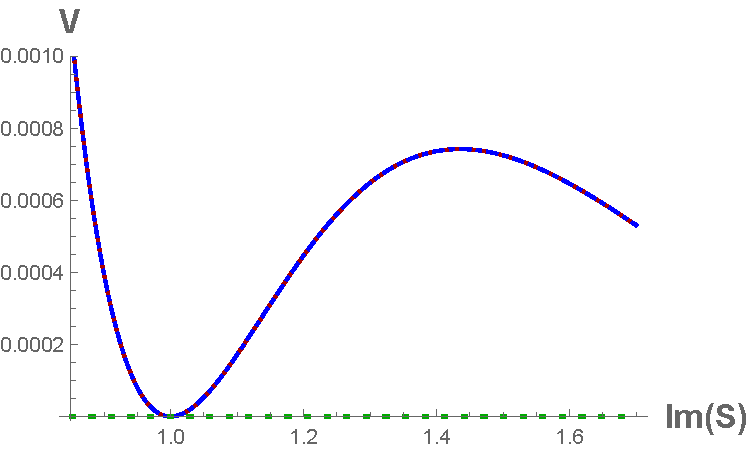
\includegraphics[scale=0.52]{quevedo_314_S_large.pdf}\qquad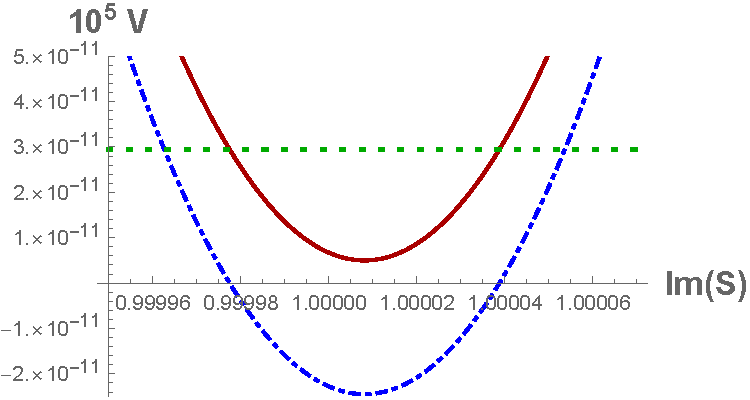
\includegraphics[scale=0.58]{quevedo_314_S_close.pdf}
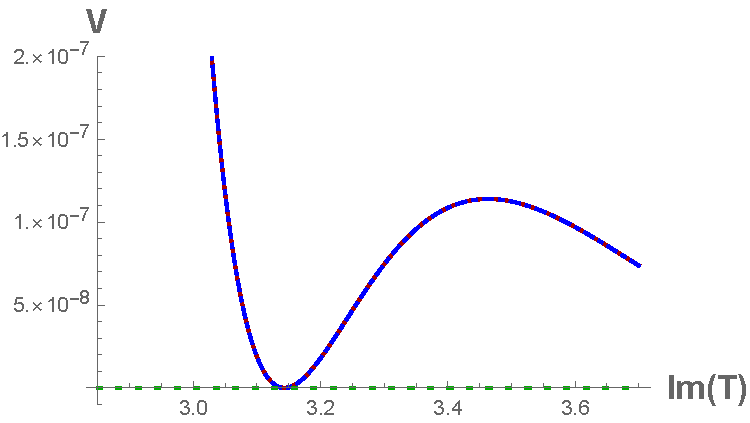
\includegraphics[scale=0.52]{quevedo_314_T_large.pdf}\qquad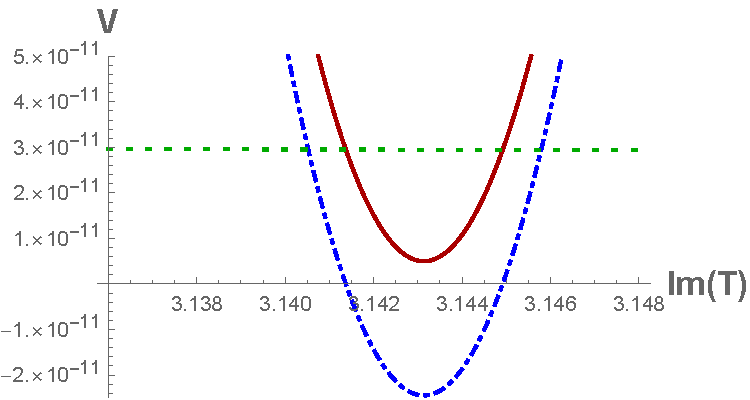
\includegraphics[scale=0.58]{quevedo_314_T_close.pdf}
\caption{2d plots of the scalar potential for both moduli directions in the 2 moduli K3-fibration model. In the large-scale plot dS and AdS are not distinguishable. The close-ups, on the right hand side, show the AdS potential (blue, dash-dotted), the de Sitter potential (red, solid) and the uplifting contribution from the anti-D3-brane (green, dotted). The shift in the position is barely noticeable with our choice of parameters.}
\label{fig:2modK32d}
\end{figure}
\begin{figure}[htb]
\centering
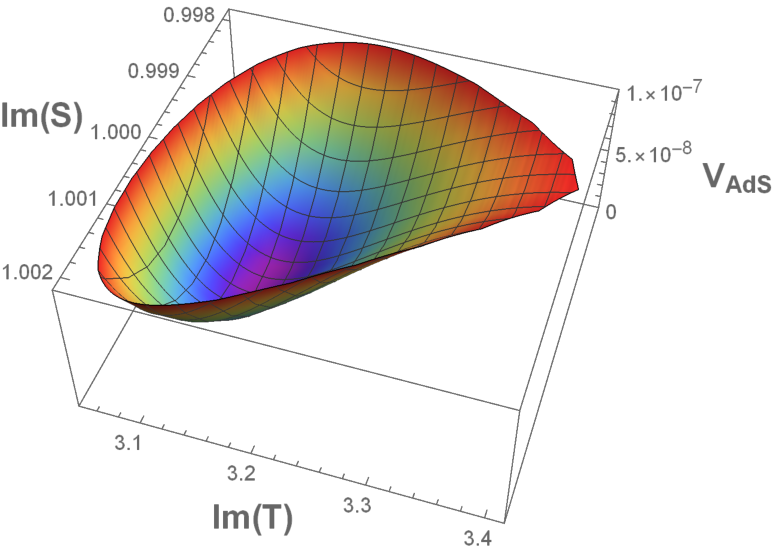
\includegraphics[scale=0.68]{quevedo_314_3D_large.pdf}
\end{figure}
\begin{figure}[htb]
\centering
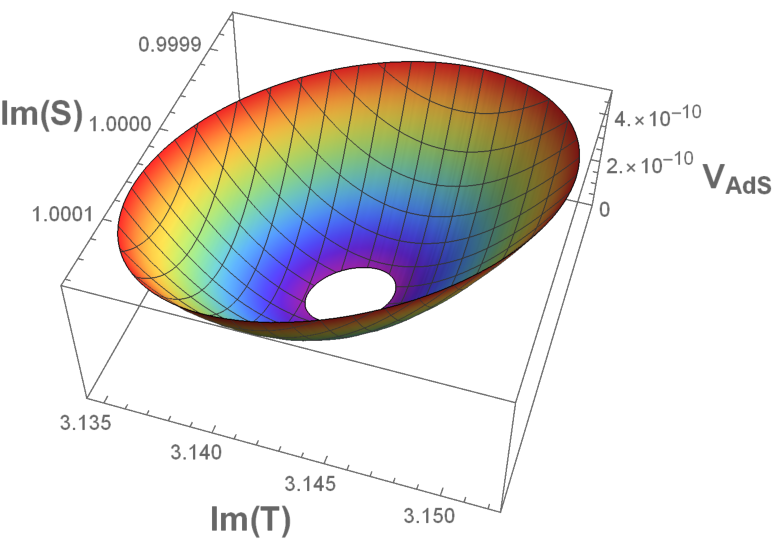
\includegraphics[scale=0.55]{quevedo_314_3D_Ads.pdf} \qquad
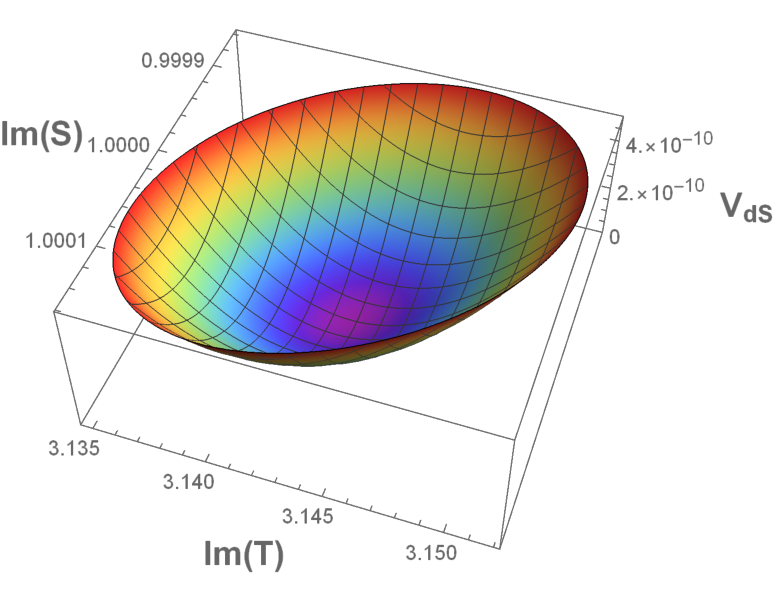
\includegraphics[scale=0.53]{quevedo_314_3D_ds.pdf}
\caption{Top: The overall shape of the scalar potential around the minimum of the 2 moduli K3 fibration. The (meta-) stability is clearly visible. The change from AdS to dS would not be visible here.\\
Bottom: Close up of the potential around the minimum for AdS (left) and dS (right).  }
\label{fig:2modK33d}
\end{figure}
Finally, the same basic picture for the masses unfolds as in type IIA, as can be seen in table \ref{tab:2modK3mass}. There we give the masses in Minkowski space and de Sitter. The masses change slightly during the process and in de Sitter the loss of the degeneracy between scalars and pseudo-scalars can be seen.
\begin{table}[htb]
\centering
\begin{tabular}{|c|c|c|}\hline
& Minkowski  & de Sitter   \\\hline
$m_1^{\,2}$ & $\; 5.22564 \cdot 10^{-2} \;$ & $\; 5.21884 \cdot 10^{-2} \;$\\\hline
$m_2^{\,2}$ & $\; 5.22564 \cdot 10^{-2} \;$ & $\; 5.21875 \cdot 10^{-2} \;$\\\hline
$m_3^{\,2}$ & $\; 1.38346 \cdot 10^{-5} \;$ & $\; 1.36014 \cdot 10^{-5} \;$\\\hline
$m_4^{\,2}$ & $\; 1.38346 \cdot 10^{-5} \;$ & $\; 1.35926 \cdot 10^{-5} \;$\\\hline
\end{tabular}
\caption{ The squared masses for the Minkowski and de Sitter case. Both the changes when going from Minkowski to de Sitter and the splitting of the degeneracy of scalars and axionic partners can be seen.}
\label{tab:2modK3mass}
\end{table}

\FloatBarrier
\paragraph{A K3 fibered Calabi Yau model} can be used for so-called fibre inflation \cite{Cicoli:2008gp,Burgess:2016owb,Kallosh:2017wku}. For this, we first consider a generalization of the 2 moduli K3 fibration we just discussed by including a blow-up mode $\tau_3$. This leads to an internal volume \cite{Cicoli:2008gp}:
\be 
\mathcal{V}_6 (\tau_i) = \alpha \left( \sqrt{\tau_1} (\tau_2 - \beta \tau_1 ) - \gamma \tau_3^{3/2} \right)\,.
\ee
The parameters $\alpha$, $\beta$ and $\gamma$ are positive and model dependent. An example for this general case is presented in detail in \cite{Cribiori:2019drf}. Here, instead, we immediately focus on the special case where $\beta = 0$, which gives
\be 
\mathcal{V}_6 (\tau_i) = \alpha \left( \sqrt{\tau_1} \tau_2  - \gamma \tau_3^{3/2} \right)\,,
\ee
or in our conventions, using $S$, $T$ and $U$ for the three complex Kähler moduli:
\be 
\mathcal{V}_6 (S,T,U) = \alpha \left( \sqrt{\left(-\rmi ( S- \bar{S})\right)} \left(-\rmi (T-\bar{T})\right) - \gamma \left(-\rmi (U-\bar{U})\right)^{3/2} \right)\,.
\ee
The physical meaning of the moduli here is as follows:
\begin{itemize}
\item $\rmim(S)$ controls the volume of the K3 fiber.
\item $\rmim(T)$ is proportional to the overall volume of the compactification manifold.
\item $\rmim(U)$ corresponds to the blow-up volume.
\end{itemize}
The special case with $\beta=0$ can be used for fibre inflation that usually relies on an LVS type uplift \cite{Balasubramanian:2005zx}. It is not our intent to construct an inflation model here but we are still inclined to investigate models that have potential for applications. Instead of the usual LVS uplift we will employ our mass production procedure with the racetrack superpotential \eqref{eq:racetrack} and the parameters given in table \ref{tab:fibrepara}. Note that we also have to set the model specific parameters $\alpha$, $\beta$ and $\gamma$.
\begin{table}[htb]
\centering
\begin{tabular}{|c|c|c|}\hline
$A_S = 1.1$ & $A_T = 1.2$ & $A_U =1.3$\\\hline
$a_S = 2.1$ & $a_T = 2.2$ & $a_U = 2.3$\\\hline
$b_S = 3.1$ & $b_T = 3.2$ & $b_U = 3.3$\\\hline
$S_0 = 1$ & $T_0 = 1$ & $U_0 = 1$\\\hline
$\alpha = 1$ & $\beta=0$ & $\gamma = \frac{1}{2} $ \\\hline
\end{tabular}
\caption{  Chosen parameters for the 3-moduli K3 fibration with $\beta = 0$.}
\label{tab:fibrepara}
\end{table}
For the downshift and uplift parameters we choose values
\bea
\Delta W_0 &= - 10^{-5}\\
\mu^4_{\text{bulk}} &= 3.10079 \cdot 10^{-10}\,,
\eea
where we once again will focus on the placement of the anti-D3-branes in the bulk. Placing the branes at the bottom of a warped throat and using $\mu^4_{\text{throat}} = 2.46069 \cdot 10^{-10}$ will produce similar results. The resulting potential is visualized in figures \ref{fig:fibre2d} and \ref{fig:fibre3d}. 

\begin{figure}[htb]
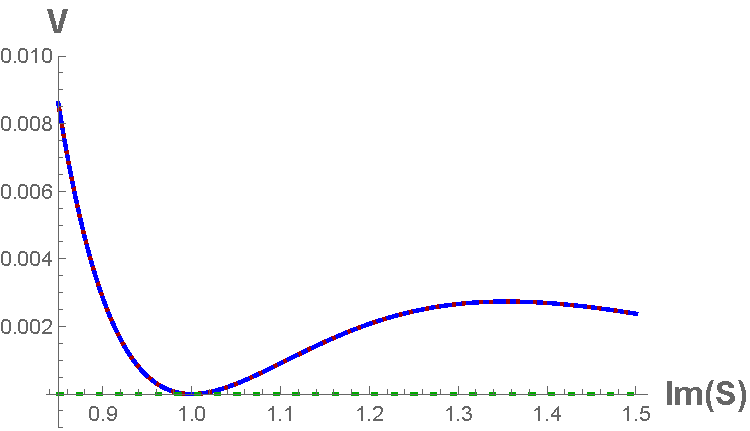
\includegraphics[scale=0.55]{fibreSLarge.pdf} \qquad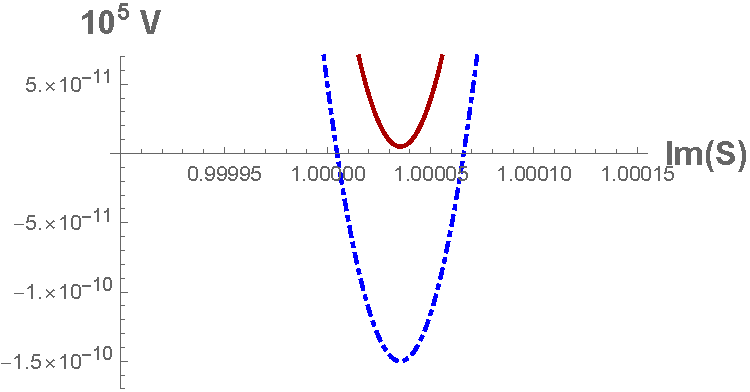
\includegraphics[scale=0.6]{fibreSClose.pdf}
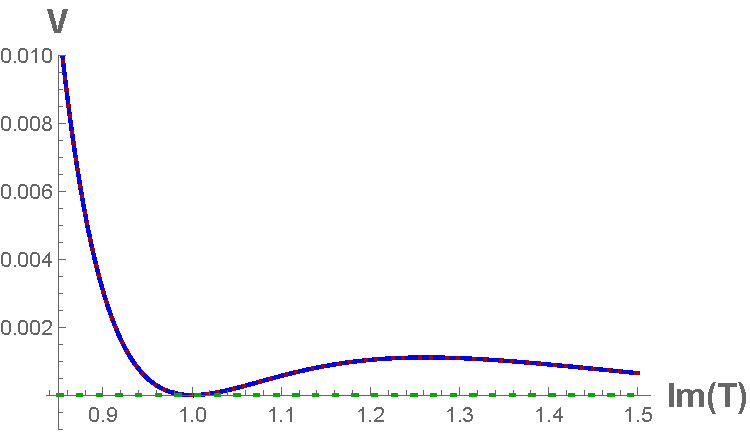
\includegraphics[scale=0.55]{fibreTLarge.pdf} \qquad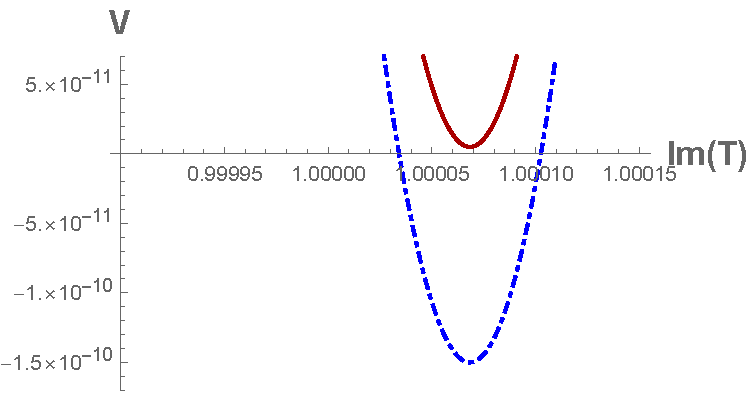
\includegraphics[scale=0.6]{fibreTClose.pdf}\\
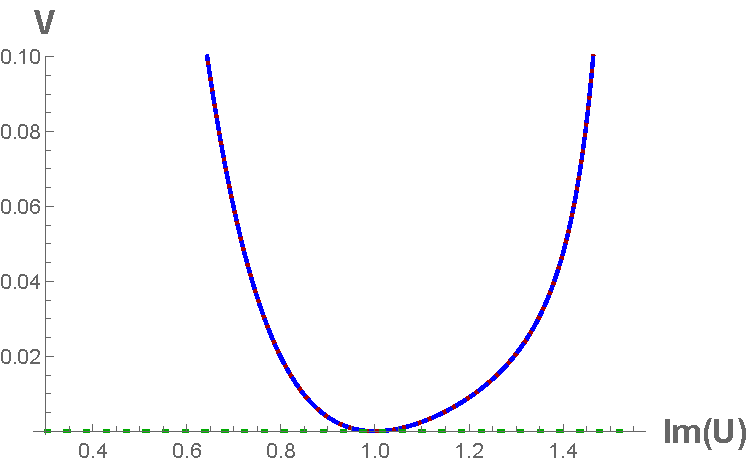
\includegraphics[scale=0.55]{fibreULarge.pdf} \qquad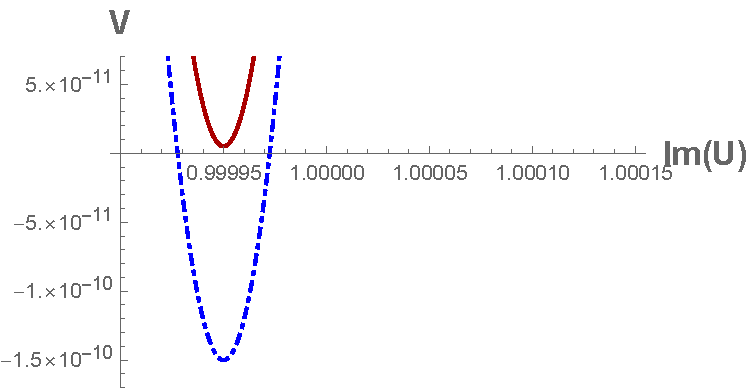
\includegraphics[scale=0.6]{fibreUClose.pdf}
\caption{2-dimenaional plots of the minimum of the K3-fibration model used for fibre inflation. The large scale pictures on the left show the AdS and dS scalar potential overlapping. On the right the close up of the minimum depicts the AdS minimum (blue, dash-dotted) being lifted to a dS minimum (red, solid). The anti-D3-brane contribution (green, dotted) is above the close up of the minimum in this case. }
\label{fig:fibre2d}
\end{figure}
\begin{figure}[htb]
\centering
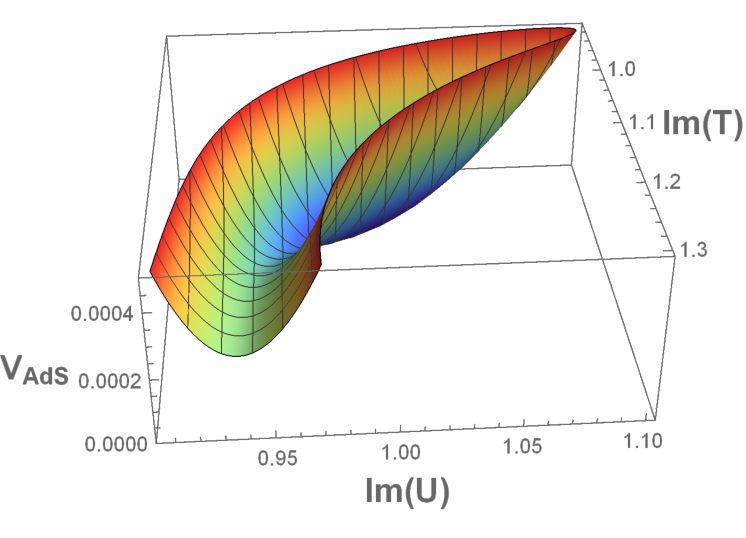
\includegraphics[scale=0.7]{fibre3DLarge}
\caption{Form of the scalar potential around the minimum of the fibre inflation model in the $\rmim(T)$ and $\rmim(U)$ slice in 3d.}
\label{fig:fibre3d}
\end{figure}

The values of the eigenvalues of the mass matrix are given in table \ref{tab:fibremass}, for Minkowski and de Sitter. Once again we find the usual picture that they change slightly and that the degeneracy of scalars and pseudo-scalars is broken in dS.
\begin{table}[htb]
\centering
\begin{tabular}{|c|c|c|}\hline
&  Minkowski  & de Sitter \\\hline
$m_1^{\,2}$ & $\; 1.01997 \cdot 10^{\;0} \,\;$ & $\; 1.01957 \cdot 10^{\;0} \,\;$\\\hline
$m_2^{\,2}$ & $\; 1.01997 \cdot 10^{\;0} \,\;$ & $\; 1.01957\cdot 10^{\;0}  \,\;$\\\hline
$m_3^{\,2}$ & $\; 1.31424 \cdot 10^{-1} \;$ & $\; 1.31344 \cdot 10^{-1} \;$\\\hline
$m_4^{\,2}$ & $\; 1.31424 \cdot 10^{-1} \;$ & $\; 1.31338 \cdot 10^{-1} \;$\\\hline
$m_5^{\,2}$ & $\; 2.44807 \cdot 10^{-2} \;$ & $\; 2.44724 \cdot 10^{-2} \;$\\\hline
$m_6^{\,2}$ & $\; 2.44807 \cdot 10^{-2} \;$ & $\; 2.44665 \cdot 10^{-2} \;$\\\hline
\end{tabular}
\caption{The squared masses for the fibre inflation model. The masses change minutely when going from Minkowski to de Sitter and the degeneracy is broken in de Sitter.}
\label{tab:fibremass}
\end{table}

\FloatBarrier
\paragraph{Our final example is based on the Fano three-fold $\mathcal{F}_{11}$} and is sometimes called a multi-hole Swiss cheese model. This manifold is topologically equivalent to a Calabi-Yau three-fold with Hodge numbers $h^{1,1} = 3$ and $h^{2,1} =111$. It has been studied in detail in \cite{Denef:2004dm}. The internal volume can be described by \cite{Cicoli:2008gp}:
\be 
\mathcal{V}_6 (\tau_i) = \frac{1}{3 \sqrt{2}} \bigg(2[\tau_1  + \tau_2 + 2 \tau_3]^{3/2} - [\tau_2 + 2 \tau_3]^{3/2} - [\tau_2]^{3/2}\bigg)\,.
\ee
Translating this to our complex Kähler moduli we obtain:
\bea
\mathcal{V}_6(S,T,U) = &\frac{1}{3 \sqrt{2}} \bigg( 2 \left[ \left(-\rmi (S-\bar{S})\right) +\left(-\rmi (T-\bar{T})\right) +2 \left(-\rmi (U-\bar{U})\right)\right]^{3/2}\\
&- \left[\left(-\rmi (T-\bar{T})\right) + 2\left(-\rmi (U-\bar{U})\right) \right]^{3/2} - \left[-\rmi (T-\bar{T})\right]^{3/2}\bigg)\,.
\eea
The procedure continues as usual with
\bea
\Delta W &= - 5 \cdot 10^{-6}\\
\mu^4_{\text{bulk}} &= 9.62862 \cdot 10^{-11}\,,
\eea
and the other parameters given in table \ref{tab:swisspara}.

\begin{table}[htb]
\centering
\begin{tabular}{|c|c|c|}\hline
$A_S = 1.1$ & $A_T = 1.2$ & $A_U =1.3$\\\hline
$a_S = 2.1$ & $a_T = 2.2$ & $a_U = 2.3$\\\hline
$b_S = 3.1$ & $b_T = 3.2$ & $b_U = 3.3$\\\hline
$S_0 = 1$ & $T_0 = 1$ & $U_0 = 1$\\\hline
\end{tabular}
\caption{ Parameter choices for the model based on the Fano 3-fold $\mathcal{F}_{11}$.}
\label{tab:swisspara}
\end{table}

As before we show 2d and 3d plot of the minimum in figures \ref{fig:swiss2d} and \ref{fig:swiss3d}. The masses obtained with these parameters are given in table \ref{tab:swissmasse}.

\begin{figure}[htb]
\center
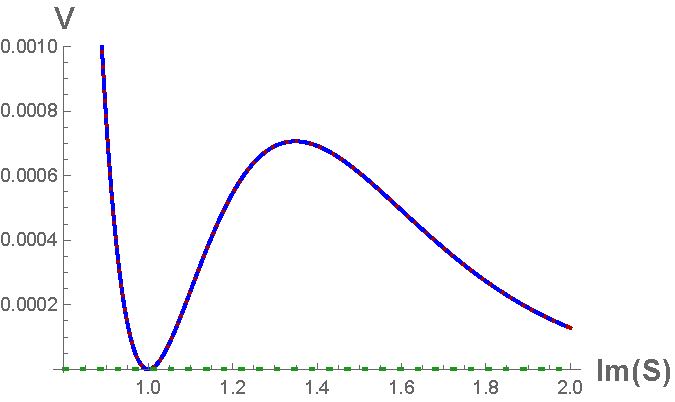
\includegraphics[scale=0.56]{quevedo_38_S_large.pdf}\qquad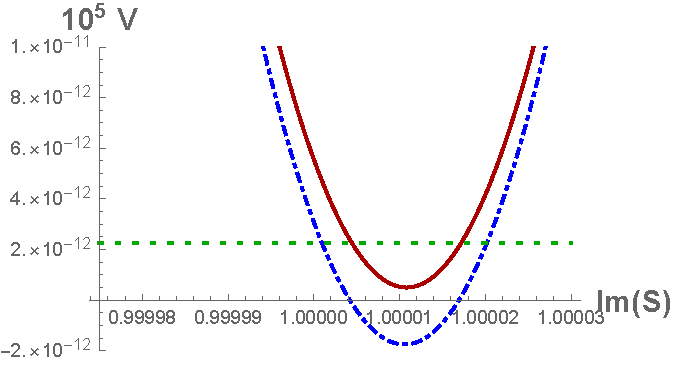
\includegraphics[scale=0.6]{quevedo_38_S_close.pdf}
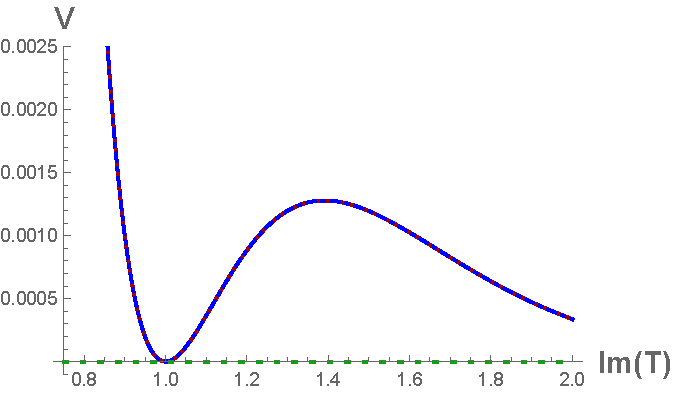
\includegraphics[scale=0.56]{quevedo_38_T_large.pdf}\qquad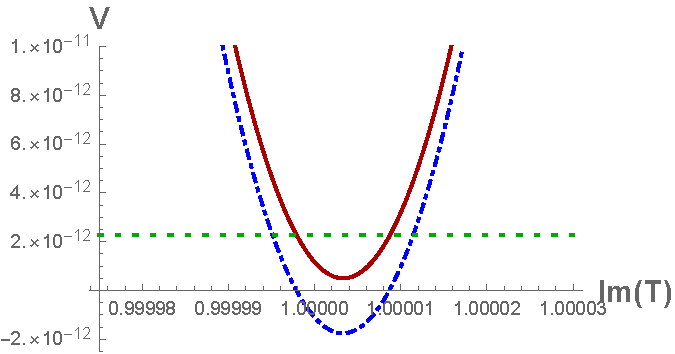
\includegraphics[scale=0.6]{quevedo_38_T_close.pdf}
\end{figure}
\begin{figure}[htb]
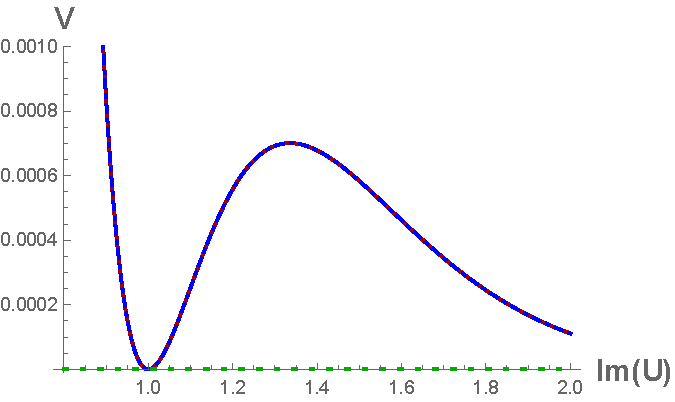
\includegraphics[scale=0.56]{quevedo_38_U_large.pdf}\qquad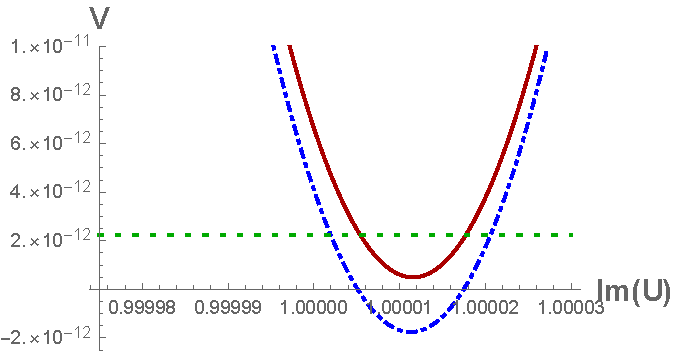
\includegraphics[scale=0.6]{quevedo_38_U_close.pdf}
\caption{2d plots of the scalar potential in the Fano three-fold model. All 3 directions show a similar meta-stable behaviour. The AdS potential (blue, dash-dotted) gets lifted to dS (red, solid) via the contribution of the ant-D3-brane (green, dotted).}
\label{fig:swiss2d}
\end{figure}

\begin{figure}[htb]
\centering
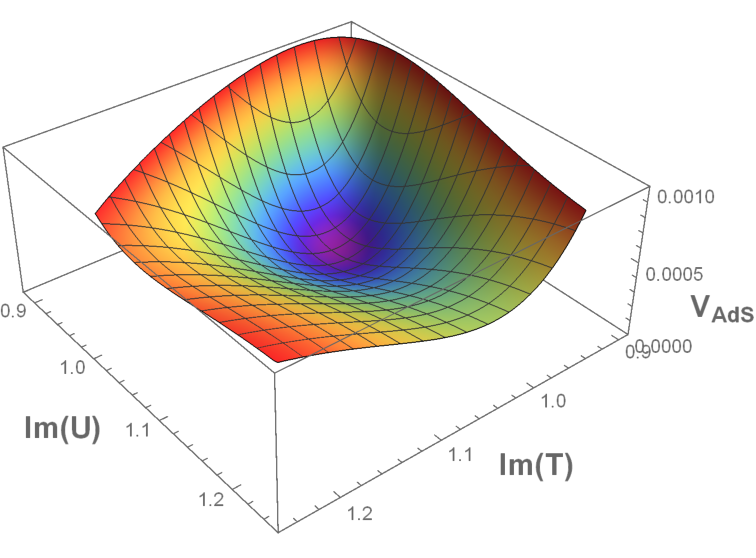
\includegraphics[scale=0.8]{quevedo_38_3D_large.pdf}
\caption{3d plot of the $\rmim(T)$ and $\rmim(U)$ slice in the Fano three-fold model with the meta-stable minimum clearly visible.}
\label{fig:swiss3d}
\end{figure}

\begin{table}[htb]
\centering
\begin{tabular}{|c|c|c|}\hline
&  Minkowski  & de Sitter \\\hline
$m_1^{\,2}$ & $\; 1.85578 \cdot 10^{-1} \;$ & $\; 1.85557 \cdot 10^{-1} \;$\\\hline
$m_2^{\,2}$ & $\; 1.85578 \cdot 10^{-1} \;$ & $\; 1.85557 \cdot 10^{-1} \;$\\\hline
$m_3^{\,2}$ & $\; 1.00760 \cdot 10^{-1} \;$ & $\; 1.00753 \cdot 10^{-1} \;$\\\hline
$m_4^{\,2}$ & $\; 1.00760 \cdot 10^{-1} \;$ & $\; 1.00753 \cdot 10^{-1} \;$\\\hline
$m_5^{\,2}$ & $\; 1.30646 \cdot 10^{-2} \;$ & $\; 1.30627 \cdot 10^{-2} \;$\\\hline
$m_6^{\,2}$ & $\; 1.30646 \cdot 10^{-2} \;$ & $\; 1.30626 \cdot 10^{-2} \;$\\\hline
\end{tabular}
\caption{Squared masses of the Fano three-fold model in Minkowski space and de Sitter.}
\label{tab:swissmass}
\end{table}

\FloatBarrier
\subsection{Models with large downshifts and uplifts}
Up until now we looked at de Sitter models that were obtained by performing small deviations from Minkowski space. This is an intuitive safe bet if one hopes to be successful. The way to quantify this is by requiring that the gravitino mass is small compared to the lightest field in the mass matrix. During the investigation of all models presented in \cite{Cribiori:2019drf} it was found that this condition might not necessarily be required. \\
First, let us mention that for small $\Delta W$ the sign did not matter too much as the downshift is proportional to its square. For large downshift the linear term becomes relevant and it is important to use $\Delta W >0$. Then it is possible to use a large downshift and a large uplift in order to obtain a stable de Sitter minimum. During this procedure the masses will now change significantly but they will stay positive, as will be shown in the example in the following. Another interesting feature ist that large uplifts allow to control the degree of supersymmetry breaking, which might be useful for certain applications.\\

As an example for a model with large shifts we return to our familiar type IIA STU model\footnote{Here we use our type IIA notation with $S$ being the axio-dilaton, $T$ the complex structure modulus and $U$ the Kähler modulus.} of section \ref{sec:massIIAexampel}. The relevant potentials \eqref{eq:massIIA7modpot} are utilized in the exact same way as before with the parameters in table \ref{tab:largpara}. Here we solved for $A_S$, $B_S$, $B_T$ and $B_U$. The downshift and subsequent uplift are given by the parameters
\be 
\Delta f_6 = 1 \qquad \text{and} \qquad \mu_1^4 = \mu_2^4 = 8.1479 \cdot 10 ^{-5}\,.
\ee
These values are several orders of magnitude larger than what we have used thus far. Nevertheless, as can be seen from figure \ref{fig:3dlargeshift} we obtain (meta-) stable minima in AdS and dS. The position of the minimum does shift significantly when going from Minkowski do anti-de Sitter and then de Sitter:
\bea 
\rmim(S):& \qquad 1 \; \to \; 1.03367 \; \to \; 1.11369 \\
\rmim(T):& \qquad 1 \; \to \; 0.13319 \; \to \; 0.51958 \\
\rmim(U):& \qquad 5 \; \to \; 4.58783 \; \to \; 3.88815 \,.
\eea
While  one does need to be careful to follow this minimum properly during the procedure there are no obstacles to do so and the procedure works out properly.
\begin{table}[htb]
\centering
\begin{tabular}{|c|c|c|}\hline
$a_S = 1$ & $a_T = 3/4$ & $a_U = 1/2$\\\hline
$b_S = 3/2$ & $b_T =5/3$ & $b_U = 2/3$\\\hline
$f_6 = 1 $ & $A_T = 3$ & $A_U =20$\\\hline
%$B_S = -19.6283$ & $B_T = 3.37627$ & $B_U =34.5146$\\\hline
$S_0 = 1$ & $T_0 = 1$ & $U_0 = 5$\\\hline
\end{tabular}
\caption{ The parameters for the IIA STU model with large downshift and uplift.}
\label{tab:largpara}
\end{table}
\begin{figure}[htb] 
%\begin{center}
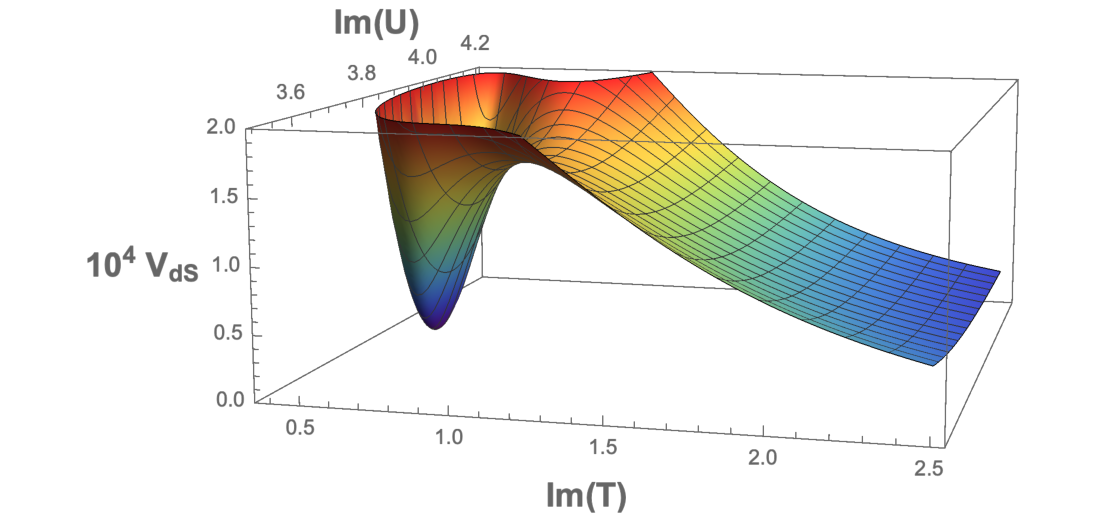
\includegraphics[scale=0.46]{STULarge1.pdf}\qquad 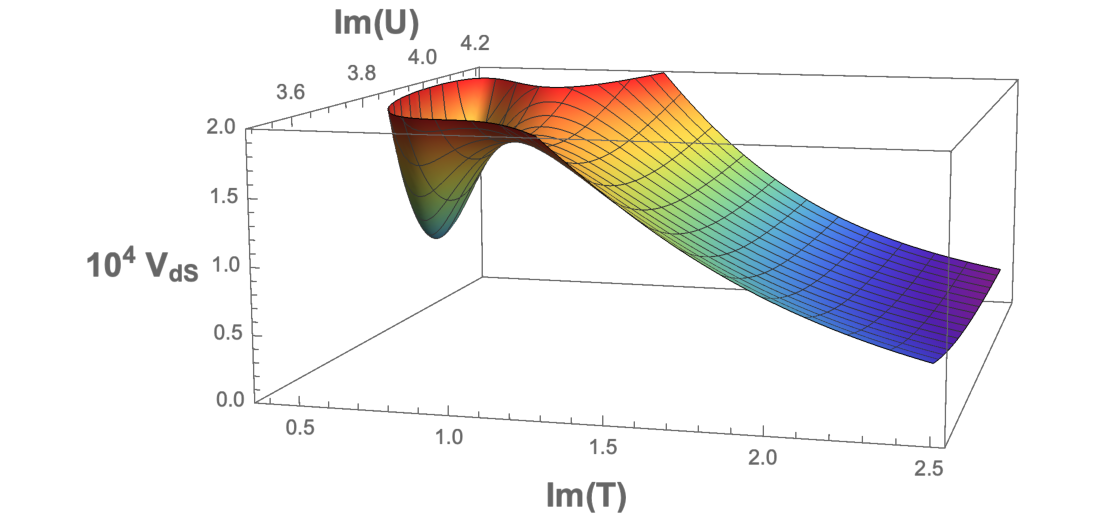
\includegraphics[scale=0.46]{STULarge2.pdf}
%\end{center}
\caption{3d plots of the STU model with large downshift and uplift in AdS (left) and dS (right). The other possible slices show similar behaviour. }
\label{fig:3dlargeshift}
\end{figure}
The eigenvalues of the mass matrix do change significantly during the procedure but minimum does not become unstable. Indeed, as can be seen from table \ref{tab:largemass} the fields become heavier. The deviation from the mass degeneracy also becomes more distinct. Still, there are no significant problems in the procedure and we obtain the desired result.
\begin{table}[htb]
\centering
\begin{tabular}{|c|c|c|}\hline
&  Minkowski  & de Sitter \\\hline
$m_1^{\,2} $ & $\; 1.07895 \cdot 10^{-2} \;$ & $\; 1.32013 \cdot 10^{-1} \;$  \\\hline
$m_2^{\,2} $ & $\; 1.07895 \cdot 10^{-2} \;$ & $\; 1.22573 \cdot 10^{-1} \;$ \\\hline
$m_3^{\,2} $ & $\; 1.29976 \cdot 10^{-3} \;$ & $\; 9.61218 \cdot 10^{-2} \;$ \\\hline
$m_4^{\,2} $ & $\; 1.29976 \cdot 10^{-3} \;$ & $\; 9.02659 \cdot 10^{-2} \;$ \\\hline
$m_5^{\,2} $ & $\; 1.05464 \cdot 10^{-4} \;$ & $\; 2.14932 \cdot 10^{-3} \;$ \\\hline
$m_6^{\,2} $ & $\; 1.05464 \cdot 10^{-4} \;$ & $\; 1.87824 \cdot 10^{-3} \;$ \\\hline
\end{tabular}
\caption{  Squared masses in the type IIA STU model with large downshift and uplift. }
\label{tab:largemass}
\end{table}

The idea of large shifts was further investigated in \cite{Linde:2020mdk} where it was shown that it is potentially possible to uplift to de Sitter even from models that do not have an AdS minimum but rather a runaway potential. 

\section{de Sitter Minima from M-theory and String Theory}
\label{sec:mtheory}
This section is based on \cite{Cribiori:2019hrb} where we considered moduli stabilization on a twisted seven torus in M-theory. Generally, this is a special case of a manifold with $G_2$-structure as $\mathbb{Z}_2 \times \mathbb{Z}_2 \times \mathbb{Z}_2 \subset G_2$. The twisted seven torus is obtained as a toroidal orbifold $X_7 = \mathbb{T}^7/(\mathbb{Z}_2 \times \mathbb{Z}_2 \times \mathbb{Z}_2)$ \cite{DallAgata:2005zlf,Duff:2010vy,Derendinger:2014wwa,Ferrara:2016fwe} with Betti numbers $(b_0,b_1,b_2,b_3) = (1,0,0,7)$. The quotient can be made non-singular by a choice of a free orbifold action. The resulting theory corresponds to a maximal rank reduction on the seven torus and gives $4d, \; \mathcal{N}=1$ supergravity with seven moduli. Finally, we introduce the twist which can be viewed as Scherk-Schwarz reduction of the initial torus.\\
In 11d one can extend the action of 11d supergravity to a form where the potentials and dual curvatures appear at the same time. This democratic form results in a pseudo-action and was studied in \cite{DallAgata:2005zlf}. In 10d the corresponding pseudo-action was proposed in \cite{Bergshoeff:2001pv}. Here, we follow \cite{DallAgata:2005zlf,Derendinger:2014wwa} in order to use these pseudo actions for moduli stabilization in 4d.\\
Going one step further, one can consider the generalized twisted seven torus \cite{Derendinger:2014wwa,Blaback:2018hdo,Villadoro:2007yq}. In these models the inclusion of KK5 and KKO5-planes in 10d or KK6 and KKO6-planes in 11d allows to lift some restrictions, like the tadpole conditions.\\
Our goal here is to use models from the generalized twisted seven torus in order to find Minkowski vacua that then can be used for the mass production procedure we already discussed \cite{Kallosh:2019zgd,Cribiori:2019drf}. I this section we will always have 7 complex moduli, corresponding to 14 real fields. Previously we used a superpotential that prominently featured non-perturbative corrections in all directions and lacked tree level flux terms. Moreover, in the mass production procedure a Kallosh-Linde type double exponent was used. Here, we will construct models that include quadratic flux terms in the superpotential and we will find not only that we can have single exponential terms in the superpotential, but also models where it is not necessary to have exponents in all directions. The connection to type IIA on a six torus can be made for some of these models. Finally, by including conjectured non-geometric fluxes \cite{Aldazabal:2006up}, we also present a model in type IIB that does not rely on any non-perturbative corrections. The origin of the required terms is not clear but can be motivated by S-duality.

\subsection{The Generalized Twisted Seven Torus}
The Kähler- and superpotential that we will use for the generalized twisted seven torus model are \cite{DallAgata:2005zlf,Derendinger:2014wwa}:
\bea 
\label{eq:mtheorypots}
K &= - \sum_{i=1}^7 \log \left( -\rmi (\Phi^i - \bar{\Phi}^i)\right)\,,\\
W &=  g_7 + \frac{1}{2} M_{ij} \Phi^I \Phi^J\, + \sum_{i=1}^7 A_i \rme ^{\rmi a_i \Phi^i},
\eea
where we already made some modifications to the superpotential. The complete perturbative part of $W$ is 
\be
W_{pert} =  g_7 + G_I \Phi^I + \frac{1}{2} M_{IJ} \Phi^I \Phi^J\,.
\ee
We have set the linear terms to zero via $G_I =0$ and introduced a single non-perturbative contribution for each field. Later on we will set some of those to zero as well, by setting the corresponding $A_I=0$. For us the relevant contributions are a seven flux $g_7$ and the terms quadratic in the moduli that come from geometric fluxes. All parameters are real and $M_{IJ}$ has a vanishing diagonal and is symmetric. Thus, it gives 21 parameters in total. In this model the non-perturbative contributions may arise from wrapping M2-branes around 3-cycles \cite{Harvey:1999as}. For $\mathbb{T} ^7/(\mathbb{Z}_2 \times \mathbb{Z}_2 \times \mathbb{Z}_2)$ seven 3 cycles are available, allowing for non-perturbative corrections in all directions.\\
The first step in the mass production procedure is to find a stable, supersymmetric vacuum state. This is done by solving $W = 0$ and $\partial_I W = 0$. Once, again we split the complex moduli $\Phi^I = \phi^I + \rmi \theta^i$ and set $\theta^i=0$, which is consistent for as long as the masses remain positive. The seven equations $\partial_I W =0$ can be solved in terms of the coefficients $A_I$ by setting:
\be 
A_I = \rmi a^{-1}_I \rme^{-\rmi a_I \Phi^I} M_{IJ} \Phi^J\,.
\ee
Then, we use $g_7$ to solve the remaining condition $W=0$, giving the desired Minkowski vacuum state. In our examples we will also consider models where no exponent appears in one or more directions. Then the solutions to the supersymmetry equations are obtained in terms of flux parameters. By inclusion of some conjectured S-dual fluxes it is even possible to find a model that does not rely on any non-perturbative corrections. It is highly non-trivial and unexpected that such a solution can been found. In order employ the mass production procedure we have to keep in mind that we require there to be no flat directions. We thus have to make sure that mass matrix in Minkowski space
\be 
V_{I\bar{J}}^{\text{Mink}} = m_{IK} K^{K\bar{K}} m_{\bar{K}\bar{J}} = \rme^K W_{IK} K^{K\bar{K}} \overline{W}_{\bar{K}\bar{J}}\,,
\ee
has no zero eigenvalues. This is different from the models considered in section \ref{sec:massprod}, since there, the double exponent superpotential guarantees that there can be no flat directions. Still, in constructing the explicit examples in \cite{Cribiori:2019hrb} and in the following, no particular tedious fine-tuning of the free parameters was necessary in order to find Minkowski solutions without flat directions.\\

For convenience, we will use our type IIA notation where
\be 
\Phi^I = \{S,T_i,U_i\}\,,\qquad i=1,2,3\,,
\ee
but note that the physical interpretation of these fields is not necessarily the same as before. We also decompose the quadratic terms in the superpotential as \cite{Derendinger:2014wwa}:
\be 
\label{eq:mtheoryW}
\frac{1}{2} M_{IJ} \Phi^I \Phi^J = S b^k U_k + U_i C^{ij} T_j + a^i \frac{U_1 U_2 U_3}{U_i} + c^i \frac{T_1 T_2 T_3}{T_i} + S d^k T_k\,.
\ee
The 21 independent components of $M_{IJ}$ are translated to $a^i$, $b^k$, $c^i$, $d^k$ and the $C^{ij}$. It is not necessary to always use all of these terms in order to obtain a Minkowski minimum and several cases will be explored in section \ref{sec:mtheoryexamples}. 

\subsection{Connection to type IIA}
\label{sec:IIAconn}
When considering type IIA string theory compactifications on $\mathbb{T}^6/(\mathbb{Z}_2 \times \mathbb{Z}_2)$ not all terms in \ref{eq:mtheoryW} are allowed \cite{Derendinger:2014wwa,Blaback:2018hdo,Villadoro:2007yq}. Namely, the terms proportional to the $c^i$ and the $d^k$ have to vanish in standard IIA orientifold compactifications. Additionally, $g_7$ gets replaced by the six-flux $f_6$. In type IIA  we can give a physical interpretation to the various terms appearing in the superpotential. 
\begin{itemize}
\item $a^i \frac{U_1 U_2 U_3}{U_i}$ are two-fluxes.
\item $U_i C^{ij} T_j$ and $S b^k U_k$ correspond to non-geometric fluxes.
\end{itemize}
There are more conditions that need to be satisfied, namely the tadpole constraints. Luckily, it is possible to include sources in order to fulfill them. The conditions are:
\begin{itemize}
\item $\sum_i a^i b^i = 0$ and $\sum_i a^i C^{ij} = 0$ that can be satisfied by $(O6/D6)$ sources.
\item $b^i C^{ij} + b^j C^{ii} = 0$ can be fulfilled by $(KK5/KKO5)$.
\item $C^{ij}C^{jk} + C^{ij} C^{jj} = 0$ gets relaxed by including $(KK5/KKO5)^\prime$.
\end{itemize}
In the various models we will discuss some of these conditions will be automatically satisfied while for others we will use them to further constrain some parameters. Then, no sources are necessary. 

\subsection{M-Theory Examples}
\label{sec:mtheoryexamples}
Here we will review explicit examples based on the potentials \eqref{eq:mtheorypots} that were discussed in detail in \cite{Cribiori:2019hrb}.
\paragraph{Including only single exponents in each direction} is the most straightforward thing we can try after exploring models with Kallosh-Linde type double exponents before. The superpotential we consider is
\be 
W_1 = g_7 + b^k S U_k + C^{ij} U_i T_j + A_S \rme^{\rmi a_S S} + \sum_i \left( A_{T_i} \rme^{\rmi a_{T_i}T_i} + A_{U_i} \rme^{\rmi a_{U_i}U_i} \right)\,.
\ee
This model has 19 free parameters, only 8 of which will be required to solve the Minkowski equations $W = 0$ and $\partial_I W = 0$ ($I = \{S, T_i, U_i \}$) at the point $S_0$, $T_{i,0}$ and $U_{i,0}$. We choose to solve for the $A_I$ and $g_7$. The remaining parameters can be used to make sure all masses are positive. Our choice of parameters can be found in table \ref{tab:3exppara} and the resulting masses are given in table \ref{tab:3expmass}.
\begin{table}[htb]
\center
\begin{tabular}{|c|c||c|c||c|c||c|c|}\hline
 $\,S_0\,$     & $1.0$   & $\,a_S\,$ & $\;1.0\,$ &$\,C^{11}\,$ & $\,0.11\,$ &  $\,C^{32}\,$ & $\,0.32\,$\\\hline
 $T_{1,0}$ & $\,1.1\,$ & $\,a_{T_1}\,$ & $\;1.1\,$ & $C^{12}$ & $0.12$ & $C^{33}$ & $0.33$ \\\hline
 $T_{2,0}$ & $1.2$ & $\,a_{T_2}\,$ & $\;1.1\,$ & $C^{13}$ & $0.13$ & $b^1$     & $0.55$\\\hline
 $T_{3,0}$ & $1.3$ & $\,a_{T_3}\,$ & $\;1.1\,$ & $C^{21}$ & $0.21$ & $b^2$     & $0.60$  \\\hline
 $U_{1,0}$ & $5.1$ & $\,a_{U_1}\,$ & $\;0.51\,$ & $C^{22}$ & $0.22$ & $b^3$     & $0.65$ \\\hline
 $U_{2,0}$ & $5.2$ & $\,a_{U_2}\,$ & $\;0.52\,$ & $C^{23}$ & $0.23$ & $\Delta g_7$ & $5 \cdot 10^{-3} $ \\\hline
 $U_{3,0}$ & $5.3$ & $\,a_{U_3}\,$ & $\;0.53\,$ & $C^{31}$ & $0.31$ & $\mu^4$ & $ 9 \cdot 10^{-9} $ \\\hline
\end{tabular}
\caption{Chosen parameters for the model with 3 single exponents.}
\label{tab:3exppara}
\end{table}
\begin{table}[htb]
\center
\begin{tabular}{|c|c|c|c|c|c|c|c|}\hline
     &$\,m_1^{\,2}\,$&$\,m_2^{\,2}\,$&$\,m_3^{\,2}\,$&$\,m_4^{\,2}\,$&$\,m_5^{\,2}\,$&$\,m_6^{\,2}\,$&$\,m_7^{\,2}\,$\\\hline
Mk & $\,0.41229\,$ & $\, 0.22090 \,$ & $\, 0.10343 \,$ & $\, 0.03087 \,$ & $\, 0.01977 \,$ & $\, 0.01275 \,$ & $\, 0.00676 \,$ \\\hline  
dS & $\, 0.41306 \,$ & $\, 0.22137 \,$ & $\, 0.10356 \,$ & $\, 0.03091 \,$ & $\, 0.01980 \,$ & $\, 0.01277 \,$ & $\,0.00677\,$ \\\hline  
\end{tabular}
\caption{The eigenvalues of the mass matrix for the model with 3 single exponents in Minkowski and de Sitter. The axions are omitted for brevity.}
\label{tab:3expmass}
\end{table}

In this model, the amount of free parameters allows us to fulfill the tadpole conditions without including sources. The conditions not automatically satisfied are:
\bea 
b^i C^{ij} + b^j C^{ii} = 0\,,\\
C^{ij} C^{jk} + C^{ik} C^{jj} = 0\,.
\eea
These conditions can, for example, be solved in terms of the $C^{ij}$ with $i \neq j$. If we keep the other parameters as before in table \ref{tab:3exppara} we obtain the masses in table \ref{tab:3expmasstad}. Satisfying the tadpole conditions without sources can be a great advantage for model building as one has to be very careful about the origins of the sources and their stability in some cases.
\begin{table}[htb]
\center
\begin{tabular}{|c|c|c|c|c|c|c|c|}\hline
     &$\,m_1^{\,2}\,$&$\,m_2^{\,2}\,$&$\,m_3^{\,2}\,$&$\,m_4^{\,2}\,$&$\,m_5^{\,2}\,$&$\,m_6^{\,2}\,$&$\,m_7^{\,2}\,$\\\hline
Mk &  $\, 0.09036 \,$  &  $\, 0.02693 \,$  &  $\, 0.01390 \,$  & $\, 0.00558 \,$ &  $\, 0.00388 \,$  &  $\, 0.00159 \,$  &  $\, 0.00063 \,$  \\\hline  
dS &  $\, 0.08982 \,$  &  $\, 0.02680 \,$  &  $\, 0.01383 \,$  & $\, 0.00555 \,$  &  $\, 0.00388 \,$  &  $\, 0.00158 \,$  &  $\, 0.00063 \,$  \\\hline   
\end{tabular}
\caption{The masses squared in the 3 exponent model where the tadpole conditions are satisfied.}
\label{tab:3expmasstad}
\end{table}

\FloatBarrier
\paragraph{Omitting the S-exponent} can be done without including any new terms. The superpotential reads
\be 
W_1 = g_7 + b^k S U_k + C^{ij} U_i T_j + \sum_i \left( A_{T_i} \rme^{\rmi a_{T_i}T_i} + A_{U_i} \rme^{\rmi a_{U_i}U_i} \right)\,,
\ee
and, because $A_S$ is absent, we solve for $b^1$ in addition to the usual parameters. Again, we use the parameters of table \ref{tab:3exppara}, except for those that are now determined by the equations $W = 0$ and $\partial_I W = 0$. The masses obtained this way are given in table \ref{tab:noSmass}.
\begin{table}[htb]
\center
\begin{tabular}{|c|c|c|c|c|c|c|c|}\hline
     &$\,m_1^{\,2}\,$&$\,m_2^{\,2}\,$&$\,m_3^{\,2}\,$&$\,m_4^{\,2}\,$&$\,m_5^{\,2}\,$&$\,m_6^{\,2}\,$&$\,m_7^{\,2}\,$\\\hline
Mk & $\, 0.40450 \,$ & $\, 0.21428 \,$ & $\, 0.10857 \,$ & $\, 0.02223 \,$ & $\, 0.01501 \,$ & $\, 0.00998 \,$ & $\, 0.00130 \,$ \\\hline  
dS & $\, 0.40513 \,$ & $\, 0.21465 \,$ & $\, 0.10870 \,$ & $\, 0.00223 \,$ & $\, 0.01503 \,$ & $\, 0.00999 \,$ & $\, 0.00130 \,$ \\\hline  
\end{tabular}
\caption{Eigenvalues of the mass matrix for the model without an exponent in the S-direction.}
\label{tab:noSmass}
\end{table}

\FloatBarrier
\paragraph{The 3 exponents in the $U_i$ directions can be left out} by including the terms proportional to $a^i$ in \eqref{eq:mtheoryW}. The superpotential becomes:
\be
W = g_7 + S b^k U_k + U_i C^{ij} T_j + a^i \frac{U_1 U_2 U_3}{U_i} + A_S \rme^{\rmi a_S S} + \sum_i  A_{T_i} \rme^{\rmi a_{T_i}T_i}\,.
\ee
Instead of the $A_{U_i}$ we now solve for the parameters $a^i$. Keeping the remaining free parameters the same as in table \ref{tab:3exppara} we find the squared masses in table \ref{tab:noUmass}.
\begin{table}[htb]
\center
\begin{tabular}{|c|c|c|c|c|c|c|c|}\hline
     &$\,m_1^{\,2}\,$&$\,m_2^{\,2}\,$&$\,m_3^{\,2}\,$&$\,m_4^{\,2}\,$&$\,m_5^{\,2}\,$&$\,m_6^{\,2}\,$&$\,m_7^{\,2}\,$\\\hline
Mk & $\, 0.06600 \,$ & $\, 0.05485 \,$ & $\, 0.02910 \,$ & $\, 0.02028 \,$ & $\, 0.01588 \,$ & $\, 0.01061 \,$ & $\, 0.00066 \,$ \\\hline  
dS & $\, 0.06615 \,$ & $\, 0.05494 \,$ & $\, 0.02914 \,$ & $\, 0.02031 \,$ & $\, 0.01590 \,$ & $\, 0.01061 \,$ & $\, 0.00066 \,$  \\\hline  
\end{tabular}
\caption{Squared masses for the case without non-perturbative corrections in the U-directions.}
\label{tab:noUmass}
\end{table}
This model is in particular interesting as it still corresponds to a type IIA model. In \cite{Cribiori:2019drf,Cribiori:2019bfx} type IIA models were studied that had only 6-form flux as perturbative contributions but relied heavily on the inclusion of non-perturbative corrections in all directions. In particular, the origin of the exponents in the U-direction required some motivation as their origin is not fully understood.

\FloatBarrier
\paragraph{Building a model without $T$ and $U$ exponents} requires the inclusion of the terms proportional  to $c^i$. The superpotential becomes
\be
W = g_7 + S b^k U_k + U_i C^{ij} T_j + a^i \frac{U_1 U_2 U_3}{U_i} + c^i \frac{T_1 T_2 T_3}{T_i} + A_S \rme^{\rmi a_S S}\,,
\ee
and we solve for $A_S$, the $a^i$ and the $c^i$ parameters. Note that this model can no longer be interpreted in terms of type IIA string theory, as discussed in section \ref{sec:IIAconn}. The parameters not set to zero or solved for are still take from table \ref{tab:3exppara} and lead to the masses in table \ref{tab:noTUmass}.
\begin{table}[htb]
\center
\begin{tabular}{|c|c|c|c|c|c|c|c|}\hline
     &$\,m_1^{\,2}\,$&$\,m_2^{\,2}\,$&$\,m_3^{\,2}\,$&$\,m_4^{\,2}\,$&$\,m_5^{\,2}\,$&$\,m_6^{\,2}\,$&$\,m_7^{\,2}\,$\\\hline
Mk & $\, 0.06964 \,$ & $\, 0.06350 \,$ & $\, 0.02158 \,$ & $\, 0.00380 \,$ & $\, 0.00210 \,$ & $\, 0.00113 \,$ & $\, 0.00083 \,$ \\\hline  
dS & $\, 0.06948 \,$ & $\, 0.06315 \,$ & $\, 0.02152 \,$ & $\, 0.00380 \,$ & $\, 0.00208 \,$ & $\, 0.00113 \,$ & $\, 0.00082 \,$  \\\hline  
\end{tabular}
\caption{Eigenvalues of the mass matrix for the model without $T$ and $U$ exponents.}
\label{tab:noTUmass}
\end{table}

\FloatBarrier
\subsection{Type IIB Examples}
In type IIB models the superpotential has contributions from F-, H- and Q-flux \cite{Aldazabal:2006up,Dibitetto:2011gm,Blaback:2013ht}, which are all well-known and established. However, it has also been conjectured that, due to S-duality, P-fluxes should appear. These terms naturally appear in gauged supergravity in 4 dimensions \cite{Dibitetto:2011gm}. Keeping only terms even in the moduli we use the following superpotential:
\bea
\label{eq:noexpW}
W =\; &a_0 + a^i \frac{U_1 U_2 U_3}{U_i} + S \left( b^i U_i + b_3 U_1 U_2 U_3 \right) \\
&+ T_k \left( C^{ik}U_i - c^k U_1 U_2 U_3\right) - S T_k \left( d^k -D^{ik}\frac{U_1 U_2 U_3}{U_i}\right)\,.
\eea
The superpotential is made up of the following contributions:
\begin{itemize}
\item $a_0$ is a constant contribution, similar to $W_0$ in previous sections.
\item $a^i \frac{U_1 U_2 U_3}{U_i}$ comes from F-flux.
\item $S \left( b^i U_i + b_3 U_1 U_2 U_3 \right)$ gives H-flux contributions.
\item $T_k \left( C^{ik}U_i - c^k U_1 U_2 U_3\right)$ represents Q-flux.
\item $- S T_k \left( d^k -D^{ik}\frac{U_1 U_2 U_3}{U_i}\right)$ are the conjectured P-fluxes.
\end{itemize}
Using \eqref{eq:noexpW} we can build a model that does not rely at all on non-perturbative terms. First, we set the $D^{ik}=0$, as they are not required. Then, we find a Minkowski vacuum without flat directions by soling for $a_0$, $a^i$, $b_3$ and $c^k$ and using the parameters in table \ref{tab:noexppara}. Following the mass production procedure we then obtain a meta-stable de Sitter point with the downshift and uplift parameters
\be 
\Delta a_0 = 5 \cdot 10^{-3}\qquad \text{and} \qquad \mu^4 = 9\cdot 10^{-9}\,.
\ee
The resulting masses are given in table \ref{tab:noexpmass}.
\begin{table}[htb]
\center
\begin{tabular}{|r|r||r|r||r|r||r|r||r|r|}\hline
$\,b^{1}$ & $\, 0.55 \,$  & $\,C^{11}$ & $ -0.11 \,$ & $\,C^{21}$ & $\, 0.21 \,$ & $\,C^{31}$ & $\, 0.31 \,$ & $\,d^{1}$ & $\, 5.1 \,$ \\\hline
$\,b^{2}$ & $\, 0.60 \,$ & $\,C^{12}$ & $\, 0.12 \,$ & $\,C^{22}$ & $ -0.22 \,$ & $\,C^{32}$ & $\, 0.32 \,$ & $\,d^{2}$ & $ -5.2 \,$ \\\hline
$\,b^{3}$ & $\, 0.65 \,$ & $\,C^{13}$ & $\, 0.13 \,$ & $\,C^{23}$ & $\, 0.23 \,$ & $\,C^{33}$ & $ -0.33 \,$ & $\,d^{3}$ & $\, 5.3 \,$ \\\hline
\end{tabular}
\caption{Parameter choices for the model without any exponents in IIB string theory/gauges supergravity.}
\label{tab:noexppara}
\end{table}

\begin{table}[htb]
\center
\begin{tabular}{|c|c|c|c|c|c|c|c|}\hline
     &$\,m_1^{\,2}\,$&$\,m_2^{\,2}\,$&$\,m_3^{\,2}\,$&$\,m_4^{\,2}\,$&$\,m_5^{\,2}\,$&$\,m_6^{\,2}\,$&$\,m_7^{\,2}\,$\\\hline
Mk & $\, 0.29074 \,$ & $\, 0.20712 \,$ & $\, 0.01075 \,$ & $\, 0.00383 \,$ & $\, 0.00287 \,$ & $\, 0.00057 \,$ & $\, 0.00016 \,$ \\\hline  
dS & $\, 0.29063 \,$ & $\, 0.20721 \,$ & $\, 0.01073 \,$ & $\, 0.00382 \,$ & $\, 0.00287 \,$ & $\, 0.00057 \,$ & $\, 0.00016 \,$  \\\hline  
\end{tabular}
\caption{Eigenvalues of the mass matrix for the IIB model without non-perturbative corrections.}
\label{tab:noexpmass}
\end{table}

\FloatBarrier
\section{de Sitter Models from Anti-Branes - Interim Summary}
In this chapter we have investigated compactifications of string theory and M-theory that result in a meta-stable de Sitter state where anti-branes were used in order to lift the vacuum energy to positive values. de Sitter spaces are of interest because the present day accelerated expansion of the universe matches very closely with the behaviour  of a de Sitter space with positive and constant, albeit very small, cosmological constant. The first model that achieved a de Sitter space from string theory by uplifting with anti-branes is the KKLT scenario \cite{Kachru:2003aw,Kachru:2003sx}. This model is based in type IIB string theory and has an uplifting contribution from an anti-D3-brane. It remains one of the best studied de Sitter constructions to date and while there have been many criticisms raised, a lot of them have also been disproved or explained.\\
In \cite{Cribiori:2019bfx} and here in section \ref{sec:IIAuplift}, we translated this mechanism to type IIA string theory. There, the uplift is performed via the inclusion of an anti-D6-brane, which is the unique choice in type IIA. The procedure relied on the inclusion of non-perturbative corrections in all moduli directions, some of which are non-standard. We motivated that they can still appear in the theory and that it is possible to use them to build meta-stable de Sitter states.\\
In section \ref{sec:massprod}, based on \cite{Kallosh:2019zgd,Cribiori:2019drf} we showed that there is a simple way to guarantee that a meta-stable de Sitter minimum can be obtained if one first constructs a Minkowski state without flat directions. We used a Kallosh-Linde type racetrack potential for all moduli directions that will automatically not have any flat directions. Under certain conditions it is then straight forward to first go to anti-de Sitter space via a small downshift and subsequently to a de Sitter via an uplifting contribution from anti-D-branes. Going to AdS first allows to avoid the fine-tuning problem encountered when going to a realistic value of the cosmological constant of $10^{-120}$ in Planck units. We showed under what conditions it is possible to predict that the masses stay positive and thus the dS vacuum state is meta-stable. Several examples in type IIA and IIB were presented.\\
Models that do have perturbative contributions to the superpotential were explored in \cite{Cribiori:2019hrb} and section \ref{sec:mtheory}. These scenarios are motivated by M-theory constructions and can be matched with type IIA or IIB models in certain special cases. Using tree-level flux contributions to the superpotential it is possible to follow the mass production procedure of de Sitter vacua without including the double exponent contribution to the superpotential in all directions. In fact, in type IIA models were presented that include non-perturbative corrections only in some directions. Perhaps most interestingly, a model that does not need exponential terms in the $U$ directions and can still be matched to type IIA string theory was presented. Including atypical fluxes, conjectured via S-duality, in IIB one finds a gauged supergravity model that even allows the procedure to work without any non-pertubative contributions to the superpotential at all.\\
The extension of the KKLT scenario to type IIA and the development of the mass production process are interesting extensions of the string model builders toolkit. The inclusion of unusual contributions in some of the models can serve as an incentive to investigate the origin of these contributions further, especially with the growing interest in semi-realistic models that aim to describe future precision cosmology experiments.


\chapter{D-Branes in 4 dimensional Supergravity}
\label{sec:antiD3}

\section{The Anti-D3-Brane in the KKLT Scenario}
The anti-D3-brane in the KKL(MM)T scenario \cite{Kachru:2003aw,Kachru:2003sx} provides the uplifting contribution to the the scalar potential that lifts the minimum from anti-de Sitter space to de Sitter. The description of the anti-brane in terms of $4d$, $\mathcal{N}=1$ supergravity has been studied in the last couple of years. Here we extend this description by including all world volume fields in a complete effective action for the KKLT scenario. As will be shown, we find that the action breaks supersymmetry spontaneously, which might be expected as the anti-D3-branes in the KKLT model can be viewed as excited states in a supersymmetric description \cite{Kachru:2002gs}.\\
The connection of the description of the anti-D3-brane to the uplfiting contributions included in the KKLT scalar potential has only been fully understood fairly recently \cite{Ferrara:2014kva,Kallosh:2014wsa,Bergshoeff:2015jxa,Kallosh:2015nia,Garcia-Etxebarria:2015lif}. Nevertheless, a full description of the action has not been found before our contribution. It consists of a bosonic part with three complex world volume scalars and an $U(1)$ gauge field and a fermionic contribution that contains four 4 dimensional fermions. In the context of flux compactifications the fermionic part has only been know up to quadratic terms \cite{Grana:2002tu,Grana:2003ek,Marolf:2003ye,Tripathy:2005hv,Martucci:2005rb,Bergshoeff:2013pia}. Naively, one would expect that the focus of the investigation would be on the bosonic part. The typical argument would be that the fermionic contributions the are given by supersymmetry. However, the bosonic contributions on the brane can be projected  out using an orientifold and thus, the focus has largely been on the fermionic part of the action \cite{Kallosh:2014wsa,Bergshoeff:2015jxa,Kallosh:2015nia,Garcia-Etxebarria:2015lif,Dasgupta:2016prs,GarciadelMoral:2017vnz}. The combination of the fermionic action with the bosonic uplifting contribution can be combined into a Volkov-Akulov type action \cite{Volkov:1973ix} which can be written using constrained superfields in $4d$, $\mathcal{N}=1$ supergravity. In \cite{GarciadelMoral:2017vnz} the action for all GKP background fields and the four world volume fermions has been derived. In \cite{Cribiori:2019hod} we extended the description to include the remaining contributions, namely the world volume scalars and the $U(1)$ gauge field. This will give a complete description of the uplifting anti-D3-brane in the KKLT background in terms of an effective $4d$, $\mathcal{N}=1$ supergravity action.

\subsection{Action of the Anti-D3-Brane in KKLT}
Before we can find the complete effective description of the anti-D3-brane we will review the action in GKP \cite{Giddings:2001yu} and KKLT\cite{Kachru:2003aw,Kachru:2003sx}. The fields that will appear in our action are 
\begin{itemize}
\item The axio dilaton $\tau = C_0 + \rmi \rme^{-\phi}$.
\item A single Kähler modulus $T$.
\item Complex structure moduli $U^A$.
\end{itemize}
The previously known bosonic and fermionic parts of the action are reviewed in the following.
\paragraph{The bosonic action} consists of a DBI and a Chern-Simons part that combine into the complete action. In $4d$ Einstein frame these can be written as: 
\bea 
S^{\text{DBI}} &= - \int d^4x \sqrt{-\text{det}\left( P \left[ g_{\mu \nu} + \rme^{-\phi/2}B_{\mu\nu}\right] + \rme^{-\phi/2} F_{\mu\nu}\right)}\,,\\
S^{\text{CS}} &= -\int P\left[(C_0 + C_2 + C_4)\wedge \rme^{B_2}\right] \wedge \rme^F\,.
\label{eq:DBICSact}
\eea 
In our conventions the string length $l_S = 2 \pi \sqrt{\alpha^\prime} = 1$, $B_2$ is the NSNS Kalb-Ramond field and $F_{\mu\nu}$ denotes the field strength of the $U(1)$ gauge field on the brane\footnote{Note that we have rescaled the $U(1)$ field strength by $2\pi$ compared to other typical conventions. Likewise, the action has been rescaled by $1/(2\pi)$ in order to remove the brane tension $T_3 = (2\pi)^{-3} (\alpha^\prime)^{-2} = 2\pi$.}. $P$ is the pullback operation onto the brane world volume.\\
The GKP background\cite{Giddings:2001yu} is warped which makes the identification of the Kähler modulus $\rmim(T)$ rather tedious \cite{Frey:2008xw}. In the case of a singe Kähler modulus a fixed overall scaling for all terms in the action exists. We will use the Ansatz \cite{deAlwis:2016cty}
\be 
ds^2 = \rme^{-6u(x)} \left(1+\frac{\rme^{-4\mathcal{A}(z)}}{\rme^{4u(x)}}\right)^{-\frac{1}{2}} g_{\mu\nu} dx^\mu dx^\nu + \rme^{2u(x)} \left(1+\frac{\rme^{-4\mathcal{A}(z)}}{\rme^{4u(x)}}\right)^{\frac{1}{6}} g_{a\bar{b}} dz^a dz^{\bar{b}}\,,
\ee
to identify $\rmim(T)$ later on. In this Ansatz the non-compact dimensions are labeled $\mu,\,\nu =0,1,2,3$ while the internal directions are $a,\,\bar{b}=1,2,3$. The six-dimensional compact volume is given by $\rme^{6u} = vol_6$ and $\mathcal{A}(z)$ is the warp factor, depending only on the internal directions. The purpose of this metric is to interpolate between the bulk region and the throat. Note that this Ansatz does not solve the mixed parts of the Einstein equations, where the non-compact and internal coordinates mix. This will, however, not have any effect on our conclusions. Since we want to investigate the anti-D3-brane action at the bottom of a strongly warped throat we are interested in the regime where $\rme^{-4\mathcal{A}}\gg \rme^{4u}$. In this limit the metric becomes
\be 
ds^2 = \rme^{-4 u(x) + 2\mathcal{A}(z)} g_{\mu\nu} dx^\mu dx^\nu + \rme^{\frac{4}{3} u(x) - \frac{2}{3} \mathcal{A}(z)} g_{a\bar{b}} dz^a dz^{\bar{b}}\,.
\ee
Utilizing this we proceed our investigation of the DBI action \cite{McGuirk:2012sb} in \eqref{eq:DBICSact}: 
\bea
S^{\text{DBI}} = - \int d^4x \sqrt{-g_4} \bigg(& \rme^{4 \mathcal{A}(H,\bar{H}) - 8 u(x)} + \frac{1}{2}  \rme^{\frac{4}{3} \mathcal{A}(H,\bar{H}) - \frac{8}{3} u(x)} g_{a\bar{b}}(H,\bar{H}) \partial_\mu H^a \partial^\mu \bar{H}^{\bar{b}} \\&+ \frac{1}{4} \rme^{-\phi(H,\bar{H})} F_{\mu\nu} F^{\mu\nu} + \cdots \bigg)\,.
\label{eq:DBIact}
\eea
Here, the $H^a$ are the  world volume scalars that give the position of the brane, entering the action via the pullback and the ellipses denote suppressed, higher order terms. In the following we will consider the brane to be sitting at some point in the strongly warped throat and then $H^a$ will denote small fluctuations around that initial position.\\
The DBI-part of the action yields all kinetic terms for the scalar fields. In $4d$, $\mathcal{N} = 1$ supergravity this this can be described using the Kähler potential \cite{DeWolfe:2002nn}:
\be 
K = -3 \log [-\rmi (T-\bar{T}) + k(H,\bar{H})]\,,
\label{eq:barD3Kpot}
\ee
with $k(H,\bar{H})$ the part of the Kähler potential that incorporates the metric of the compact manifold:
\be 
\partial_{H^a} \partial_{\bar{H}^{\bar{b}}} k(H,\bar{H}) \approx \frac{1}{6} \rme^{\frac{4}{3}(\mathcal{A}+u)} g_{a\bar{b}}\,.
\ee
Subleading terms are again neglected \cite{Baumann:2007ah}. Importantly, the no-scale structure of the Kähler potential is not violated by this contribution. The volume of the internal manifold depends on the open and closed string degrees of freedom and gets modified by $k(H,\bar{H})$:
\be 
vol_6 = \rme^{6u} = \left(-\rmi (T-\bar{T}) + k(H,\bar{H})\right)^{\frac{3}{2}}\,.
\ee
The Cern-Simons part of the action simplifies in the GKP background \cite{Giddings:2001yu} to
\[S^{\text{CS}} = -\int \left(\frac{1}{2} C_0 (H,\bar{H}) F\wedge F + C_4 (H,\bar{H}) \right)\,\]
where one has  to keep in mind that the contributions from $B_2$ and $C_2$ are projected out by the orientifold in our setup. We then expand the quantities around the position of the brane where we use, as mentioned before, $H^a$ as the distance from the brane sitting at $(H^a,\bar{H}^a) = (0,0)$ in the warped throat. To leading order we get:
\bea 
S^{\text{CS}} &= -\int \left(\frac{1}{2} C_0 (H,\bar{H}) F\wedge F + C_4 (H,\bar{H}) \right)\\
&=-\int \left( \frac{1}{2} C_0(0,0)F\wedge F + C_4(0,0)+ \cdots\right)\,.
\eea 
We then use that $C_0(0,0) = \rmre(\tau) $ and $C_4(0,0) = \alpha(z,\bar{z}) \sqrt{-g_4} dx^0 \wedge dx^1 \wedge dx^2 \wedge dx^3$ and find for the Chern-Simons action:
\be 
S^{\text{CS}}=-\int d^4x \sqrt{-g_4} \left(-\frac{1}{8 \sqrt{-g_4}}\rmre(\tau) \epsilon^{\mu \nu \rho \sigma} F_{\mu \nu} F_{\rho \sigma} + \alpha(H,\bar{H}) + \cdots \right)\,,
\label{eq:CSact}
\ee
In order to combine the two parts of the bosonic action we first combine the first term in the DBI action \eqref{eq:DBIact} with the second term in the CS action \eqref{eq:CSact} to:
\be 
\Phi_\pm := \rme^{4\mathcal{A}(H,\bar{H})-8u} \pm \alpha(H,\bar{H})\,,
\ee
where the sign difference is for branes (minus) and anti-branes (plus). For the D3-brane the equations of motion in the GKP background enforce  $\rme^{4\mathcal{A}(H,\bar{H})-8u} = \alpha(H,\bar{H})$ and thus $\Phi_-=0$ but for the anti-brane the DBI and CS contributions add up and we find the combined action for the anti-D3-brane to be
\bea 
S^{\overline{D3}}_{\text{bosonic}}= -\int d^4x \sqrt{-g_4} \bigg(&2 \rme^{4\mathcal{A}(H,\bar{H})-8u} + \frac{1}{2} \rme^{\frac{4}{3} \mathcal{A}(H,\bar{H})-\frac{8}{3} u(x)} g_{a\bar{b}} \partial_\mu H^a \partial^\mu \bar{H}^{\bar{b}} \\&+ \frac{1}{4} \rmim(\tau)F_{\mu\nu} F^{\mu \nu} - \frac{1}{8 \sqrt{-g_4}} \epsilon^{\mu \nu \rho \sigma} F_{\mu \nu} F_{\rho \sigma} + \cdots \bigg)\,.
\label{eq:simpbosact}
\eea 
We find that, combining the DBI with the CS action, we get a typical Maxwell term for the $U(1)$ gauge field.  For a D3-brane in our setup we would have preserved $\mathcal{N}=1$ supersymmetry and one would use a gauge kinetic function $f(\tau)=-\rmi \tau$ for the supergravity description. The gauge kinetic function has to be holomorphic and may only depend on the axio-dilaton. The coupling at the brane for the $U(1)$ gauge interaction is given by $\rmre(f(\tau)) = \rmim(\tau) = \rme^{-\phi}$. On the other hand, $\rmim(f(\tau)) = - \rmre(\tau) = -C_0$, controlling the theta term of the Maxwell part of the action. If we now want to consider our anti-D4-brane, the Chern-Simons action comes with a sign difference and thus it seems that, in order to match equation \eqref{eq:CSact}, we would need an anti-holomorphic gauge kinetic function, satisfying $f(\bar{\tau})= \rmi \bar{\tau})$. Supersymmetry does not allow for this since $\tau$ is part of an unconstrained chiral multiplet. The resolution of this issue is one of the main points of this chapter and will be discussed later on in \ref{sec:sugraact}. The important physical conclusion will be that the anti-D3-brane preserves non-linear $\mathcal{N}=1$ supersymmetry.\\
Moving on, we can identify a scalar potential
\be 
V^{\overline{D3}}(H,\bar{H}) = \Phi_+ = 2 \rme^{4\mathcal{A}(H,\bar{H})-8u}\,,
\ee
that gives the attraction of the brane towards the bottom of the warped throat, as there the warp factor $\mathcal{A}$ is minimized. As usual, we expand the scalar potential in terms of the $H^a$ and $\bar{H}^{\bar{b}}$ around the point of attraction:
\bea 
V^{\overline{D3}}(H,\bar{H}) = 2 \rme^{4 \mathcal{A}_0-8u_0} \big( 1 &+ 2 H^a H^b \partial_{H^a} \partial_{H^b} \mathcal{A}_0 + 4 H^a \bar{H}^{\bar{b}} \partial_{H^a} \partial_{\bar{H}^{\bar{b}}} \mathcal{A}_0  \\&+ 2 \bar{H}^{\bar{a}} \bar{H}^{\bar{b}} \partial_{\bar{H}^{\bar{a}}} \partial_{\bar{H}^{\bar{b}}} \mathcal{A}_0 + \cdots \big)\,.
\eea
The quantities with index ``$zero$" are evaluated at $H=0$ and we once more neglect higher order contributions, suppressed by the string scale \cite{McGuirk:2012sb}. From the first term in this expression we get the typical uplifting term from an anti-D3-brane in a warped throat which scales like $1/vol_6^{4/3}$ \cite{Kachru:2003sx}.  \\
Before we continue a remark about the KKLT scenario is in order. The volume modulus in a GKP background is flat and together with the scalar potential of the anti-D3-brane this would lead to an instability for the Kähler modulus. This gets remedied via the inclusion of non-perturbative corrections, usually from gaugino condensation on D7-branes in the bulk. The argument then is that, since the non-perturbative effect happens in the bulk and we consider the anti-D3-brane at the bottom of a highly warped throat, these contributions can safely be neglected. Issues around these non-perturbative corrections have been discussed in the literature to a great extend \cite{Moritz:2017xto,Moritz:2018sui,Kallosh:2018wme,Moritz:2018ani,Kallosh:2018psh,Gautason:2018gln,Hamada:2018qef,Kallosh:2019axr,Kallosh:2019oxv,Hamada:2019ack,Carta:2019rhx,Gautason:2019jwq,Kachru:2019dvo} and, as of now, it seems reasonable to proceed along following the argument given here.

\paragraph{The fermionic part of the anti-$D3$-brane action} has to contain a Goldstino, responsible for the spontaneous breaking of supersymmetry by the anti-brane. The goal of this part of the thesis is  to offer a complete description of the anti-D3-brane in the KKLT setup in the language of $4d$, $\mathcal{N}=1$ supergravity. For this, the Goldstino will be described using a constrained superfield, to be precise it will be contained in a nilpotent chiral field. \\
Before we come to the fermionic action of the anti-$D3$-brane we need to figure out how the anti-D3-brane action contains the Goldstino. General Dp-brane action in flux backgrounds are know only up to quadratic orders in fermions \cite{Grana:2002tu,Grana:2003ek,Marolf:2003ye,Tripathy:2005hv,Martucci:2005rb,Bergshoeff:2013pia}. Discussion focused on the anti-D3-brane in this context can be found in \cite{Kallosh:2014wsa,Bergshoeff:2015jxa,GarciadelMoral:2017vnz,McGuirk:2012sb}. \\
There are four world volume fermions on the anti-D3-brane, part of the $SU(3)$ holonomy group of the internal manifold. One singlet $\lambda$ and three $\chi^i$, forming a triplet. The behavior of these fermions is determined by the imaginary  sefl dual (ISD) part 
\be 
G_3^{\text{ISD}} = \frac{1}{2} \left( G_3 - \rmi \star_6 G_3 \right)\,,
\ee
of the background 3-flux \cite{Bergshoeff:2015jxa,McGuirk:2012sb} :
\be 
G_3 = F_3 - \rmi \rme^{-\phi} H_3 = dC_2 - \left(C_0 + \rmi \rme^{-\phi} \right) H_3\,.
\ee
The flux gives rise to the following contributions:
\begin{itemize}
\item The $(0,3)$-flux gives the mass of the singlet $\lambda$.
\item The interactions between the singlet $\lambda$ and the triplet $\chi^i$ are determined by non-primitive $(2,1)$-flux.
\item The primitive $(2,1)$-flux gives the masses for the triplet $\chi^i$.
\end{itemize}
In a supersymmetric GKP background the anti-D3-brane is the sole source of supersymmetry breaking and then $\lambda$ will be identified as the Goldstino. It then does not mix with the fermion triplet $\chi^i$ and does not receive a mass \cite{Bergshoeff:2015jxa}.\\
If the background already has broken supersymmetry there is a Gukov-Vafa-Witten (GVW) superpotential \cite{Gukov:1999ya} 
\be 
W_{\text{GVW}} = \int G_3 \wedge \Omega
\label{eq:GVWpot}
\ee
that is non-zero. Here, the characteristic 3-form $\Omega$ of the Calabi-Yau gives rise to an F-term for the modulus $T$:
\be 
D_T W_{\text{GVW}} = K_T W_{\text{GVW}} \neq 0\,,
\ee
where the Kähler-covariant derivative with respect to $T$ acting on $W$ is: $D_T W = \partial_T W + (\partial_T K ) W = K_T W$. It follows that $G_3$ has to contain a non-vanishing $(0,3)$ contribution which leads to spontaneous supersymmetry breaking due to the background itself. In this scenario a closed string fermion will be identified as the Goldstino. Adding an anti-D3-brane to such a background $\lambda$ would no longer be the Goldstino and, in fact, will get a mass from the $(0,3)$ part of the 3-flux $G_3$.\\
Our interest here is the KKLT scenario where, in addition to a non-vanishing GVW superpotential \eqref{eq:GVWpot}, we have non-perturbative corrections also depending on the Kähler modulus $T$ of form\footnote{See also section \ref{sec:kklt}.}:
\be 
W_{\text{np}} = A \rme^{\rmi a T}\,.
\ee
$A$ can, in general, depend on the moduli but, under certain conditions, we can neglect this as those terms are suppressed. The non-perturbative corrections allow us to find a supersymmetric solution to 
\be 
D_T \left( W_{\text{GVW}} + W_{\text{np}} \right)=0\,
\ee
which will give a supersymmetric AdS vacuum with $\partial_T W_{\text{np}} = - K_T (W_{\text{GVW}} + W_{\text{np}})$. If we add one ore more anti-D3-branes to this setup we can lift the AdS minimum to dS. However, then the anti-brane is the source of supersymmetry breaking and needs to come with a massless Goldstino. We saw, however, that the background has non-zero $(0,3)$ flux which means the fermion singlet $\lambda$ obtains a non-vanishing mass term. Futhermore, all $\chi^i$ also obtain masses and thus can't act as the Goldstino either \cite{Bergshoeff:2015jxa}. The solution to this peculiar problem is that the $(0,3)$ part of the $G_3$ flux localizes on the source of the non-pertubative contributions \cite{Baumann:2010sx,Dymarsky:2010mf}. Namely, the stack of $D7$-branes that is localized in the bulk of the internal manifold, as opposed to the location of the anti-$D3$-brane at the bottom of a warped throat. If the flux is then pulled back onto the anti-brane the contribution vanishes due to the warping. Then, the fermion singlet $\lambda$ does not obtain a mass and can act as the Goldstino. Note however that, once we go beyond the probe limit, this will not be exactly true anymore. The backreaction of the uplifting anti-$D3$-brane onto the geometry will shift the Kähler modulus $T$ away from the position of the supersymmetric minimum and then $D_TW\neq0$. The Goldstino then becomes a combination of the singlet $\lambda$ and the fermionic partner of $T$.\\
With this discussion out of the way we go on to investigate the couplings of the four fermions provided by the anti-$D3$-brane to the moduli $\tau$, $T$ and $U^a$ from the closed string sector. The fermionic action of the anti-$D3$-brane \cite{Bergshoeff:2015jx,GarciadelMoral:2017vnz,Grana:2002tu,McGuirk:2012sb} to quadratic order in the world-sheet fermions is given to be \cite{Bergshoeff:2015jx,Martucci:2005rb,Bergshoeff:2005yp}:
\bea 
S_{\text{fermionic}}^{\overline{D3}} = 2 \int d^4x & \sqrt{-g_4} \bigg[ \rme^{4\mathcal{A} - 8u} \bar{\theta}\Gamma^\mu \left( \nabla_\mu - \frac{1}{4} \rme^\phi F_\mu \tilde{\Gamma}_{0123}\right)\theta\\
&+ \frac{1}{8\cdot 4!} \bar{\theta} \bigg(\rme^{\frac{16}{3} \mathcal{A} - \frac{32}{3} u} \Gamma^{\mu mnpq}F_{\mu mnpq} - 2 \rme^{\frac{8}{3} \mathcal{A} - \frac{16}{3} u} \Gamma^{\mu\nu\rho mn} F_{\mu\nu\rho mn}\bigg) \tilde{\Gamma}_{0123}\theta\\
&- \frac{\rmi}{24} \rme^{6\mathcal{A} - 12u} \rme^{\frac{1}{2} \phi} \left( G_{mnp}^{\text{ISD}} - \bar{G}_{mnp}^{\text{ISD}}\right) \bar{\theta} \Gamma^{mnp} \theta \bigg]\,,
\label{eq:fermact}
\eea
where we are in Einstein frame, as per usual. Greek letters label the non-compact directions $0,1,2,3$ and Latin letters the internal directions $4,5,6,7,8,9$. $\theta$ is the Majorana-Weyl spinor of type IIB theory with 16 components and we will decompose it into $4d$ Weyl spinors \cite{Bergshoeff:2015jxa,Grana:2002tu}. The gamma matrix $\Gamma$ has unwarped but curved indices while $\tilde{\Gamma}$ has flat indices. In supergravity language \cite{Freedman:2012zz} the fermions are an $SU(3)$ singlet $P_L\lambda$ and three fermions $P_L\chi^i$, forming a triplet. In \cite{Bergshoeff:2015jxa} the kinetic and the $G$-flux part of \eqref{eq:fermact} were considered in a fixed background and we will use these results here. There it was found that all other terms vanish. Here, we consider a dynamical background where these terms will give important contributions \cite{Cribiori:2019hod}.\\
First of we will consider the spin connection term where we adopt the convention to put a tilde on flat quantities and indices. It is given to be:
\be
\bar{\theta} \Gamma^\mu \nabla_\mu \theta = \bar{\theta} \Gamma^\mu \left(\partial_\mu + \frac{1}{4} \omega_\mu^{\,\tilde{a}\tilde{b}} \tilde{\Gamma}_{\tilde{a}\tilde{b}} + \frac{1}{4} \omega_\mu^{\,i\ib} \tilde{\Gamma}_{i\ib}\right) \theta\,,
\ee
where the indices run over $\tilde{a},\tilde{b} = 0,1,2,3$ and $i,\ib=1,2,3$. Terms with mixed indices in the spin connection, like $\omega_\mu^{\,\tilde{a}i}$, vanish and thus are omitted. In the above expression the first two terms form the usual covariant derivative while the last term introduces an interaction of the fermions and the complex structure moduli $U^A$. In order to write the spin connection in terms of the vielbein and the moduli we note that our metric is block diagonal, consisting of the $4d$ block of the non-compact directions and a $6d$ block of the internal manifold. This immediately tells us that the vielbein is also block diagonal. Then, the internal part of the vielbein then satisfies
\be 
e^a_i g_{a\bar{b}} e^{\bar{b}}_{\ib} = \delta_{i\ib}\,.
\ee
Since the geometry of the compact Calabi-Yau is described by the Kähler modulus $T$ and the complex structure moduli $U^A$ this means that the ``internal" vielbein $e^a_i$ is a function of those moduli. Furthermore, the holomorphic 3-form $\Omega_{abc}=\epsilon_{ijk} e^i_a e^j_b e^k_c$ of the CY manifold does not depend on the $\bar{U}^A$ we know that $e^i_a$ and its inverse can only be functions of $T$, $\bar{T}$ and $U^A$. Thus, we write:
\be 
\partial_\mu e^a_i = (\partial_T e^a_i)\partial_mu T + (\partial_{\bar{T}} e^a_i) \partial_\mu \bar{T} + (\partial_{U^A} e^a_i) \partial_\mu U^A\,.
\ee
The Kähler modulus gives the overall volume of the CY manifold and since we only have one such modulus the volume has to depend on some power of $(T-\bar{T})$, to leading order and thus:
\be 
\partial_T e^a_i = -\partial_{\bar{T}} e^a_i \propto e^a_i\,.
\ee
With this the internal part of the spin connection simplifies to
\be 
\omega_\mu^{i\ib} = e^{\bar{a}i}\partial_\mu e^\ib_{\bar{a}} - e^{a\ib} \partial_\mu e^i_a = e^{\bar{a}i}(\partial_{\bar{U}^A} e^\ib_{\bar{a}} ) \partial_\mu \bar{U}^A - e^{a\ib} (\partial_{U^A} e^i_a)\partial_\mu U^A\,.
\label{eq:spincon}
\ee
This expression can be further simplified due to the fact that we only have a single Kähler modulus and thus only one $(1,1)$ form. We can use the spin connection in order to define a 2-form. If it is in cohomology it has to be proportional to the Kähler form $J$ of the Calabi-Yau manifold. In flat indices this means it is proportional to $\delta_{i\ib}$:
\be 
\omega_{\mu i\ib}\, e^i_a e^\ib_{\bar{b}} \propto \delta_{i\ib} e^i_a e^\ib_{\bar{b}}\,.
\ee
With this we can use $\omega_\mu^{i\ib} \tilde{\Gamma}_{i\ib} = 1/3 \omega_\mu^{i\ib} \delta_{i\ib} \delta^{j\jb} \tilde{\Gamma}_{j\jb}$ to write the following fermionic contribution that has not been considered in earlier works:
\bea
\bar{\theta} \Gamma^\mu \omega_\mu^{i\ib} \tilde{\Gamma}_{i\ib} \theta  
&= \frac{1}{3}\omega_\mu^{i\ib} \delta_{i\ib} \delta^{j\jb} \tilde{\Gamma}_{j\jb} \\
&= \frac{1}{3} \omega_\mu^{k\bar{k}} \delta_{k\bar{k}} \left( 3 \bar{\lambda} P_R \gamma^\mu \lambda - \delta_{i\jb} \bar{\chi}^\jb P_R \gamma^\mu \chi^i\right)\\
&= \frac{1}{3} \delta_{i\ib} \left( e^{\bar{a}i} (\partial_{\bar{U}^A} e^\ib_{\bar{a}} ) \partial_\mu \bar{U}^A - e^{a\ib} (\partial_{U^A} e^i_a) \partial_\mu U^A\right)\left( 3 \bar{\lambda} P_R \gamma^\mu \lambda - \delta{j\jb} \bar{\chi}^\jb P_R \gamma^\mu \chi^j\right)\,.
\eea
The next new contribution comes from the $F_\mu$ term in \eqref{eq:fermact}. Keeping in mind that $F_\mu = \partial_\mu C_0 = \partial_\mu \rmre(\tau)$ it is straight forward to compute:
\bea
\rme^\phi F_\mu \bar{\theta} \Gamma^\mu \tilde{\Gamma}_{0123} \theta &= \frac{(\partial_\mu \rmre(\tau)}{\rmim(\tau)} \bar{\theta}\Gamma^\mu \tilde{\Gamma}_{0123} \theta\\
&=-\rmi \frac{(\partial_\mu \rmre(\tau)}{\rmim(\tau)} \left( \bar{\lambda} P_R \gamma^\mu \lambda + \delta_{i\jb} \bar{\chi}^\jb P_R \gamma^\mu \chi^i\right)\,.
\eea
There are two more new contribution in \eqref{eq:fermact} that we need to investigate, both of the related to $C_4$. The first comes from the derivative coupling to the axion $C_4$. For this we need to know that a Calabi-Yau manifold with a single Kähler modulus has one $(2,2)$-form $Y_{2,2}$. The normalization of this form is such that it evaluates to $1$ when integrated over the 4-cycle $\Sigma_4$. The volume or Kähler modulus $T$ is made up of this 2-form and $J\wedge J$, with $J$ the characteristic 2-form of the Calabi-Yau. Since $T$ is described in $4d$ supergravity via a chiral multiplet it furthermore has to be holomorphic. Using $Y_{2,2}$ to build a basis we find that the Kähler modulus is given as:
\bea
T :&= \int_{\Sigma_4} \left( C_4 - \frac{\rmi}{2} J\wedge J\right)\\
&=\int_{\Sigma_4} c_4(x^\mu) Y_{2,2} + \rmi \rmim(T) \int_{\Sigma_4} Y_{2,2}\,,
\eea
where we also read of that $c_4(x^\mu)\, Y_{2,2} = -c_4(x^\mu)\, [2 \rmim(T)]^{-1} J\wedge J$. We can now use that $\rmi e_i^u e_\ib^{\bar{u}} J_{u\bar{u}} = \delta_{i\ib}$, with curved indices $u$ and $\bar{u}$ to find the first contribution from $C_4$ to the fermionic action of the anti-$D3$-brane:
\bea 
\frac{1}{4!} \rme^{\frac{4}{3}\mathcal{A} - \frac{8}{3} u} \bar{\theta} \Gamma^{\mu npqr} F_{\mu npqr} \theta 
&= \frac{\rmre(T)}{2\rmim(T)} \bar{\theta} \delta_{i\ib}\delta_{j\jb}\Gamma^\mu \tilde{\Gamma}^{i\ib j\jb}\tilde{\Gamma}_{0123} \theta\\
&= -\rmi \frac{\partial_\mu \rmre(T)}{\rmim(T)} \left( 3\bar{\lambda} P_R \gamma^\mu \lambda - \delta_{i\jb} \bar{\chi}^\jb P_R\gamma^\mu \chi^i \right)\,.
\eea
The remaining term related to $C_4$ can be related to the above one due to the self-duality of $dC_4$ in $10d$. Using this property one finds that
\be 
F_{\mu npqr} \Gamma^{\mu npqr} = -2 \rme^{\frac{8}{3} \mathcal{A} + \frac{16}{3} u} F_{\mu\nu \rho mn} \Gamma^{\mu \nu \rho mn} \tilde{\Gamma}_\star\,.
\ee

Finally, we can combine all parts from above in order to find the complete fermionic part of the anti-$D3$-brane action up to total derivatives:
\bea 
S_{\text{fermionic}}^{\overline{D3}} = 2 \int d^4x \sqrt{-g_4} \rme^{4\mathcal{A}-8u} 
\bigg[& \bar{\lambda} P_R \gamma^\mu \nabla_\mu \lambda + \delta_{i\jb} \bar{\chi}^\jb P_R \gamma^\mu \nabla_\mu \chi^i\\
+& \frac{\rmi}{4} \frac{\left(\partial_\mu \rmre(\tau)\right)}{\rmim(\tau)} \left( \bar{\lambda} P_R \gamma^\mu \lambda + \delta_{i\jb} \bar{\chi}^\jb P_R \gamma^\mu \chi^i\right)\\
-& \frac{\rmi}{4} \frac{\left(\partial_\mu \rmre(T)\right)}{\rmim(T)} \left(3 \bar{\lambda} P_R \gamma^\mu \lambda - \delta_{i\jb} \bar{\chi}^\jb P_R \gamma^\mu \chi^i\right)\\
+& \frac{1}{12} \omega_\mu^{k\bar{k}} \delta_{k\bar{k}} \left(3 \bar{\lambda} P_R \gamma^\mu \lambda - \delta_{i\jb} \bar{\chi}^\jb P_R \gamma^\mu \chi^i\right)\\
+&  \frac{1}{2} m \bar{\lambda} P_L \lambda + m_i \bar{\lambda} P_L \chi^i + \frac{1}{2} m_{ij} \bar{\chi^i}P_L \chi^j + \text{c.c.}\bigg]\,,
\label{eq:simpfermact}
\eea
where we wrote everything in terms of $4d$ spinors. As discussed, the masses depend on the the imaginary self dual 3-flux $G_3^{\text{ISD}}$. They are given as:
\bea 
m =&\, \rmi \,\frac{\sqrt{2}}{12}  \rme^{2\mathcal{A}-4 u}\, \rme^{\frac{\phi}{2}} \bar{\Omega}^{abc}\bar{G}_{abc}^{\text{ISD}}\,,\\
m_i =& - \frac{\sqrt{2}}{4} \rme^{2\mathcal{A}-4 u}\, \rme^{\frac{\phi}{2}} e_i^a \bar{G}_{ab\bar{c}}^{\text{ISD}} J^{b\bar{c}}\,,\\
m_{ij} =& \,\rmi \,\frac{\sqrt{2}}{8} \rme^{2\mathcal{A}-4 u}\, \rme^{\frac{\phi}{2}} \left(e_i^c e_j^d + e_j^c e_i^d \right) \Omega_{abc}g^{a\bar{a}}g^{b\bar{b}} \bar{G}_{d\bar{a}\bar{b}}\,.
\label{eq:fermmass}
\eea
Since we consider the KKLT setup with gaugino condensation on a stack of $D7$-branes in the bulk of the internal manifold, the pullback of the $G_3$-flux onto the anti-brane does vanish. Furthermore, in this background the $(2,1)$ part of $G_3^{\text{ISD}}$ is primitive and thus $G_{ab\bar{c}}^{\text{ISD}} \, J^{b\bar{c}} = 0$ and thus we find that, for our particular setup, two of the mass terms from above vanish:
\bea 
m = &\, 0\\
m_i = &\, 0\,.
\eea
As already discussed, this means that $\lambda$ remains massless and is the Goldstino related to supersymmetry breaking. The fermion triplet $\chi^i$ meanwhile does acquire non-zero masses. Hence, we have a unique Goldstino arising from the source of supersymmetry breaking, namely the fermion singlet $\lambda$.

\paragraph{The complete anti-$D3$-action for the KKLT model} from the perspective of string theory is the sum of the bosonic part \eqref{eq:simpbosact} and the fermionic contribution \eqref{eq:simpfermact}, with the masses $m$ and $m_i$ set to zero:
\bea 
S^{\overline{D3}} 
=& S^{\overline{D3}}_{\text{bosonic}} + S^{\overline{D3}}_{\text{fermionic}}\\
=& - \int d^4x \sqrt{-g_4} \bigg[ 2 \rme^{4\mathcal{A}-8u} + \frac{1}{2} \rme^{\frac{4}{3} \mathcal{A}-\frac{8}{3}u}\partial_\mu H^a \partial^\mu \bar{H}^{\bar{b}}\\
&\qquad\qquad\qquad\;\;\; + \frac{\rmim(\tau)}{4} F_{\mu\nu}F^{\mu\nu} - \frac{\rmre(\tau)}{8} \frac{\epsilon^{\mu\nu\rho\sigma}}{\sqrt{-g_4}} F_{\mu\nu}F_{\rho\sigma}\bigg]\\
& + 2 \int d^4x \sqrt{-g_4} \rme^{4\mathcal{A}-8u} \bigg[ \bar{\lambda} P_R \gamma^\mu \nabla_\mu \lambda + \delta_{i\jb} \bar{\chi}^\jb P_R \gamma^\mu \nabla_\mu \chi^i\\
&\qquad\qquad\qquad\qquad\qquad + \frac{\rmi}{4} \frac{\left(\partial_\mu \rmre(\tau)\right)}{\rmim(\tau)} \left( \bar{\lambda} P_R \gamma^\mu \lambda + \delta_{i\jb} \bar{\chi}^\jb P_R \gamma^\mu \chi^i\right)\\
&\qquad\qquad\qquad\qquad\qquad - \frac{\rmi}{4} \frac{\left(\partial_\mu \rmre(T)\right)}{\rmim(T)} \left(3 \bar{\lambda} P_R \gamma^\mu \lambda - \delta_{i\jb} \bar{\chi}^\jb P_R \gamma^\mu \chi^i\right)\\
&\qquad\qquad\qquad\qquad\qquad + \frac{1}{12} \omega_\mu^{k\bar{k}} \delta_{k\bar{k}} \left(3 \bar{\lambda} P_R \gamma^\mu \lambda - \delta_{i\jb} \bar{\chi}^\jb P_R \gamma^\mu \chi^i\right)\\
&\qquad\qquad\qquad\qquad\qquad + \frac{1}{2} m_{ij} \bar{\chi}^i P_L \chi^j + \frac{1}{2} \bar{m}_{\ib\jb} \bar{\chi}^\ib P_R \chi^\jb\bigg]\,.
\label{eq:simpbraneact}
\eea

\subsection{The $D3$-Brane Action and Supergravity}
Even though our goal is to describe the anti-$D3$-brane action in the KKLT background it will be useful to first have a look at the supersymmetric action of the $D3$-brane. The results of this section will proof useful  for the investigation of the anti-$D3$-brane case. In particular, we will match the action with the standard $\mathcal{N}=1$ supergravity action for a single vector multiplet and three chiral multiplets because for the $D3$-brane \eqref{eq:simpbosact} reduces exactly to that. First, the ``uplift" term of the bosonic action vanishes for the supersymmetric $D3$-brane as do the fermionic mass terms. Taking into account the sign flip in the RR-fields only one vector multiplet, containing $\lambda$ and $A_\mu$, and three chiral multiplets with $H^a$ and $\chi^a := e^a_i \chi^i$ remain. The $D3$-brane action is given as:
\bea 
S^{D3}
=& S^{D3}_{\text{bosonic}} + S^{D3}_{\text{fermionic}}\\
=& - \int d^4x \sqrt{-g_4} \bigg[ \frac{1}{2} \rme^{\frac{4}{3} \mathcal{A}-\frac{8}{3}u}\partial_\mu H^a \partial^\mu \bar{H}^{\bar{b}}\\
&\qquad\qquad\qquad\;\;\; + \frac{\rmim(\tau)}{4} F_{\mu\nu}F^{\mu\nu} - \frac{\rmre(\tau)}{8} \frac{\epsilon^{\mu\nu\rho\sigma}}{\sqrt{-g_4}} F_{\mu\nu}F_{\rho\sigma}\bigg]\\
& + 2 \int d^4x \sqrt{-g_4} \rme^{4\mathcal{A}-8u} \bigg[ \bar{\lambda} P_R \gamma^\mu \nabla_\mu \lambda + \delta_{i\jb} \bar{\chi}^\jb P_R \gamma^\mu \nabla_\mu \chi^i\\
&\qquad\qquad\qquad\qquad\qquad - \frac{\rmi}{4} \frac{\left(\partial_\mu \rmre(\tau)\right)}{\rmim(\tau)} \left( \bar{\lambda} P_R \gamma^\mu \lambda + \delta_{i\jb} \bar{\chi}^\jb P_R \gamma^\mu \chi^i\right)\\
&\qquad\qquad\qquad\qquad\qquad + \frac{\rmi}{4} \frac{\left(\partial_\mu \rmre(T)\right)}{\rmim(T)} \left(3 \bar{\lambda} P_R \gamma^\mu \lambda - \delta_{i\jb} \bar{\chi}^\jb P_R \gamma^\mu \chi^i\right)\\
&\qquad\qquad\qquad\qquad\qquad + \frac{1}{12} \omega_\mu^{k\bar{k}} \delta_{k\bar{k}} \left(3 \bar{\lambda} P_R \gamma^\mu \lambda - \delta_{i\jb} \bar{\chi}^\jb P_R \gamma^\mu \chi^i\right)\bigg]\,.
\label{eq:d3act}
\eea
\paragraph{First we will investigate the derivative coupling of the fermions to $\tau$.} The chiral multiplets containing the fermions do not carry any $U(1)$ charge but couple due to the Kähler covariant derivative to all scalars. The relevant part of the supergravity action is \cite{Freedman:2012zz}:
\bea
\mathcal{L}^{\text{SUGRA}} \supset &-\delta_{i\jb}\bar{\chi}^\jb P_R \gamma^\mu \left(\partial_\mu - \frac{1}{4}[\partial_\mu \tau\partial_\tau K - \partial_\mu \bar{\tau}\partial_{\bar{\tau}} K] \right) \chi^i\\
&-\frac{1}{2} \delta_{i\jb} \bar{\chi}^\jb P_R \gamma^\mu \Gamma^i_{k\tau}\partial_\mu \tau \chi^k - \frac{1}{2} \delta_{i\jb} \bar{\chi}^i P_L \gamma^\mu \Gamma^\jb_{\bar{k}\bar{\tau}} \partial_\mu \bar{\tau} \chi^{\bar{k}}\,.
\eea 
If we choose the Kähler potential for $\tau$ to be
\be 
K^{(\tau)} = - \log [-\rmi (\tau -\bar{\tau})]\,,
\ee
we obtain exactly the coupling proportional to $\partial_\mu \rmre(\tau)$ in \eqref{eq:d3act} from the square brackets above. Furthermore, the prefactor also is correct which tells us that the mixed index Christoffel symbols $\Gamma^i_{j\tau}$ have to be zero.
\paragraph{For the couplings to $\partial_\mu \rmre(T)$} we have to investigate the very similar looking part of the Lagrangian
\bea
\mathcal{L}^{\text{SUGRA}} \supset & - \delta_{i\jb} \bar{\chi}^\jb P_R \gamma^\mu \left( \partial_\mu -\frac{1}{4} [\partial_\mu T \partial_T K - \partial_\mu \bar{T} \partial_{\bar{T}} K]\right) \chi^i\\
&- \frac{1}{2} \delta_{i\jb} \bar{\chi}^\jb P_R \gamma^\mu \Gamma^i_{kT} \partial_\mu T \chi^k - \frac{1}{2} \delta_{i\jb} \bar{\chi}^i P_L \gamma^\mu \Gamma^{\jb}_{\bar{k}\bar{T}} \partial_\mu \bar{T} \chi^{\bar{k}}\,
\eea
now, with non vanishing contributions form the Christoffel symbols in the direction of $T$. In the limit of large volume we can find the corresponding Christoffel symbols from the Kähler potential \eqref{eq:barD3Kpot} is approximately
\be 
\Gamma^{i}_{jT} \approx \frac{\rmi}{2 \rmim(T)}\,.
\ee
Together with the derivatives action on the Kähler potential all contributions combine correctly and match \eqref{eq:d3act} including coefficients.
\paragraph{In a similarly straight forward manner we can find the coupling of $\tau$ to $\lambda$} from the supergravity action. For the $D3$-brane the gauge kinetic function is $f(\tau) = -\rmi \tau$ and the kinetic term of the gaugino is normalized such that its prefactor is $\rmre(f) = \rmim(\tau) = \rme^{-\phi}$. Thus, we have to rescale the fermion singlet like $\lambda = \rme^{-\phi/2} \lambda^\prime$, which does not lead to any new derivative terms since $\bar{\lambda} \gamma^\mu \lambda =0$ for $4d$ Majorana spinors. The supergravity action for the rescaled singlet $\lambda^\prime$ is:
\bea 
\mathcal{L}^{\text{SUGRA}} \supset &-\frac{1}{2} \rmre(f) \bar{\lambda}^\prime \gamma^\mu \left( \partial_\mu + \frac{1}{4} [\partial_\mu \tau \partial_\tau K - \partial_\mu \bar{\tau} \partial_{\bar{\tau}} K ] \gamma_\star \right) \lambda^\prime\\
&+ \frac{\rmi}{4} \partial_\mu \rmim(f)\bar{\lambda}^\prime \gamma_\star \gamma^\mu \lambda^\prime\,,
\eea
which reproduces the coupling of $\lambda$ to $\partial_\mu \rmre(\tau)$ in the $D3$-brane action.
\paragraph{The terms coupling the gaugino to the modulus $T$} do not involve any Christoffel symbols. Again, using $\lambda^\prime$ we can write the standard supergravity action and the terms, when compared to \eqref{eq:d3act}, match up to a different prefactor that is cause by the lack of the Christoffel symbols:
\be
\mathcal{L}^{\text{SUGRA}} \supset - \frac{1}{2} \rmre(f) \bar{\lambda}^\prime \gamma^\mu \left( \partial_\mu \frac{1}{4} [\partial_\mu T \partial_T K - \partial_\mu \bar{T} \partial_{\bar{T}} K]\gamma_\star\right) \lambda^\prime\,.
\ee
\paragraph{The final terms to analyze contain the complex structure moduli $U^A$.} The spin connections \eqref{eq:spincon} has two independent parts, since they are proportional to $\partial_\mu U^A$ and $\partial_\mu \bar{U}^A$, individually. By an analogous reasoning as below \eqref{eq:spincon} we conclude that both terms are proportional to $\delta_{i\ib}$. Hence,  we can write
\bea
\partial_{U^A} e^i_v 
&= - e^i_{w} (\partial_{U^A} e^{w\ib} ) e_{v\ib}\\
&= -\frac{1}{3} e^j_w (\partial_{U^A} e^{w\jb} ) \delta_{j\jb} \delta^{i\ib} e_{v\ib}\\
&= -\frac{1}{3} e^j_w (\partial_{U^A} e^{w\jb} ) \delta_{j\jb}  e^i_{v}\,,
\eea
where we used that $\partial_\mu e^i_v e^{v\ib} = 0$ and $v,w,\cdots = 1,2,3$ are curved and warped indices. We can related this to the $(3,0)$-form $\Omega$ of the Calabi-Yau manifold in the following way:
\bea
\partial_{U^A} \Omega &= \frac{1}{3! \cdot 3!} \partial_{U^A} \left( e^i_v e^j_w e^k_x \epsilon_{ijk} dz^v \wedge dz^w \wedge dz^x\right)\\
&= \frac{3}{3! \cdot 3!} \left(\partial_{U^A}  e^i_v\right) e^j_w e^k_x \epsilon_{ijk} dz^v \wedge dz^w \wedge dz^x\\
&= - \frac{1}{3! \cdot 3!} e^l_t \left(\partial_{U^A} e^{t\jb}\right) \delta_{l\jb} e^i_v e^j_w e^k_x \epsilon_{ijk} dz^v \wedge dz^w \wedge dz^x\\
&= -e^j_w \left(\partial_{U^A} e^{w\jb} \right) \delta_{j\jb} \Omega\,.
\label{eq:partomgexp}
\eea
In order to eventually match this with the component action of the $D3$-brane we will expand the 3-form $\Omega$ in a cohomology basis as:
\be 
\Omega = Z^K \alpha_K - F_K \beta^K\,,
\ee

with the 3-form basis given by $\alpha_K$ and $\beta^K$ that satisfy $\int \alpha_K \wedge \beta^L = \delta^L_K$. The $Z^K$ and $F_K$ are functions of the complex structure moduli $U^A$. The expansion of $\Omega$ in conjecture with \eqref{eq:partomgexp} tells us that:

\bea 
\partial_{U^A} Z^K &= - e^j_v \left(\partial_{U^A} e^{v\jb} \right) \delta_{j\jb} Z^K\,,\\
\partial_{U^A} F_K &= -e^j_v \left(\partial_{U^A} e^{v\jb}\right) \delta_{j\jb} F_K\,.
\eea

The Kähler potential for the complex structure moduli is given in terms of the 3-form $\Omega$ and can be written using the expansion above:

\bea 
K^{(U)} &= - \log \left[ -\rmi \int \Omega \wedge \bar{\Omega} \right] \\
&= - \log \left[ \rmi (Z^K \bar{F}_K - \bar{Z}^K F_K ) \right] \,.
\eea
Finally, we can use this to write the relevant part of the spin connections using the Kähler potential $K^{(U)}$ as:
\bea 
\omega_\mu^{i\ib} \delta_{i\ib} &= \delta_{i\ib} \left( e^{\bar{a}i} (\partial_{\bar{U}^A} e^{\ib}_{\bar{a}}) \partial_\mu \bar{U}^A - e^{a\ib} (\partial_{U^A} e^i_a )\partial_\mu U^A\right)\\
&= \partial_{U^A} K^{(U)} \partial_\mu U^A - \partial_{\bar{U}^A} K^{(U)} \partial_\mu \bar{U}^A\,.
\eea
Before we can use this result to match the component action \eqref{eq:d3act} with a standard supergravity expression we need to propose a fitting Kähler potential. One might naively propose 
\be
K = - \log\left[-\rmi (\tau-\bar{\tau})\right] - \log\left[-\rmi \int \Omega \wedge \bar{\Omega}\right] - 3 \log \left[-\rmi(T-\bar{T})  + k(H,\bar{H})\right]\,,
\ee
this, however, is incapable of reproducing the correct $D3$-brane action. In order to find the correct expression, we note that the coupling of the fermions $\lambda$ and $\chi^i$ to $\partial_\mu \rmre(U^A)$ has the same prefactor as the coupling to $\partial_\mu \rmre(T)$. Hence, the complex structure part has to couple in the same way to the chiral multiplets as the Kähler sector in the supergravity action. The Kähler potential
\bea 
K =& - \log\left[-\rmi (\tau-\bar{\tau})\right] - 3 \log \left[-\rmi(T-\bar{T}) \left(-\rmi\int \Omega \wedge \bar{\Omega}\right)^{\frac{1}{3}} + k(H,\bar{H})\right]\\
=&  - \log\left[-\rmi (\tau-\bar{\tau})\right] - \log\left[-\rmi \int \Omega \wedge \bar{\Omega}\right] - 3 \log \left[-\rmi(T-\bar{T})  + \frac{k(H,\bar{H})}{\left(-\rmi\int \Omega \wedge \bar{\Omega}\right)^{\frac{1}{3}}}\right]\,,
\label{eq:deKpot}
\eea
does reproduce all the required couplings to $\partial_{\mu} \rmim(\tau)$, $\partial_\mu \rmim(T)$, $\chi^i$ and $\lambda^\prime$, via standard supergravity terms. Dropping, as above, the terms containing $k(H,\bar{H})$ the relevant supergravity pieces are:

\bea 
\mathcal{L}^{\text{SUGRA}} \supset &-\delta_{i\jb} \bar{\chi}^\jb P_R \gamma^\mu \left( \partial_\mu - \frac{1}{4} \left[\partial_\mu U^A \partial_{U^A} K - \partial_\mu \bar{U}^A \partial_{\bar{U}^A} K \right]\right)\chi^i\\
&- \frac{1}{2} \delta_{i\jb} \bar{\chi}^\jb P_R \gamma^\mu \Gamma^i_{kU^a} \partial_\mu U^A \chi^k-\frac{1}{2} \delta_{i\jb} \bar{\chi}^i P_L \gamma^\mu \Gamma^\jb_{\bar{k}\bar{U}^A} \partial_\mu \bar{U}^A \chi^{\bar{k}}\\
&-\frac{1}{2} \rmre(f)\bar{\lambda}^\prime \gamma^\mu \left( \partial_\mu + \frac{1}{4} \left[\partial_\mu U^A \partial_{U^A} K - \partial_\mu \bar{U}^A \partial_{\bar{U}^A} K\right]\gamma_\star\right)\lambda^\prime\,.
\eea

As a final note we remark that, in order to produce the correction terms involving the world volume scalars, we require

\be
\partial_{H^a}\partial_{\bar{H}^{\bar{b}}} k(H,\bar{H}) \approx \frac{1}{6} \rme^{\frac{4}{3} (\mathcal{A} + u )} \left(-\rmi \int \Omega \wedge \bar{\Omega} \right)^{\frac{1}{3}} g_{a\bar{b}}\,.
\ee





\chapter{The de Sitter Swampland Conjecture}
{\bf includes the papers: dS Extrema and Refined Swampland Conjecture}


\chapter{Summary and Outlook}

\section{Summary}

\section{Outlook}

\newpage
\section*{Acknowledgements}
During the course of my doctoral studies I have been funded by an FWF grant with the number P 30265, a DOC grant of the Austrian Academy of Sciences and via the Doctoral College Particles  and Interactions with the project  number W1252-N27. My extended stay at Stanford University was made possible by an Austrian Marshall Plan Fellowship.\\
I would like to offer my sincerest thanks to my advisor Timm Wrase, for all his help and patience in all things related to my doctorate, both physical and organizational. His explanations thought me more than any book could ever have.\\
Many thanks to Niccol\`o Cribiori for many explanations, discussions and encouragement. Many thanks also to Andreas Banlaki for stimulating discussions and to Abhiram Kidambi for forcing me to consider topics beyond my comfort.\\
Special thanks to Renata Kallosh and Andrei Linde for the warm welcome at the Stanford Institute for Theoretical Physics. The discussions with you opened my eyes in many regards.\\
Furthermore I would like to thank David Andriot, Thomas Van Riet and Antoine Van Proeyen for the fruitful collaborations and kind help offered and Anton Rebhan as well as all the people at the Institute  for theoretical Physics at TU Wien for all their continued support.\\
Personal thanks go to all my friends and family for their continuous support, especially to Lukas Lüftinger for being a pillar of support when needed.\\
To my wife, Anneliese, I cannot offer sufficient thanks for supporting me over so many years but I will try my best.\\
Finally, to my parents, I am thankful for encouraging me to pursue my dreams and supporting me each step of the way.

\newpage
\singlespace
\bibliographystyle{JHEP}
\bibliography{refs}
%\bibliography{refs}
\end{document}












